%% bare_jrnl.tex
%% V1.4b
%% 2015/08/26
%% by Michael Shell
%% see http://www.michaelshell.org/
%% for current contact information.
%%
%% This is a skeleton file demonstrating the use of IEEEtran.cls
%% (requires IEEEtran.cls version 1.8b or later) with an IEEE
%% journal paper.
%%
%% Support sites:
%% http://www.michaelshell.org/tex/ieeetran/
%% http://www.ctan.org/pkg/ieeetran
%% and
%% http://www.ieee.org/

%%*************************************************************************
%% Legal Notice:
%% This code is offered as-is without any warranty either expressed or
%% implied; without even the implied warranty of MERCHANTABILITY or
%% FITNESS FOR A PARTICULAR PURPOSE! 
%% User assumes all risk.
%% In no event shall the IEEE or any contributor to this code be liable for
%% any damages or losses, including, but not limited to, incidental,
%% consequential, or any other damages, resulting from the use or misuse
%% of any information contained here.
%%
%% All comments are the opinions of their respective authors and are not
%% necessarily endorsed by the IEEE.
%%
%% This work is distributed under the LaTeX Project Public License (LPPL)
%% ( http://www.latex-project.org/ ) version 1.3, and may be freely used,
%% distributed and modified. A copy of the LPPL, version 1.3, is included
%% in the base LaTeX documentation of all distributions of LaTeX released
%% 2003/12/01 or later.
%% Retain all contribution notices and credits.
%% ** Modified files should be clearly indicated as such, including  **
%% ** renaming them and changing author support contact information. **
%%*************************************************************************


% *** Authors should verify (and, if needed, correct) their LaTeX system  ***
% *** with the testflow diagnostic prior to trusting their LaTeX platform ***
% *** with production work. The IEEE's font choices and paper sizes can   ***
% *** trigger bugs that do not appear when using other class files.       ***                          ***
% The testflow support page is at:
% http://www.michaelshell.org/tex/testflow/



\documentclass[journal]{IEEEtran}

% Some very useful LaTeX packages include:
% (uncomment the ones you want to load)


% *** MISC UTILITY PACKAGES ***
%
%\usepackage{ifpdf}
% Heiko Oberdiek's ifpdf.sty is very useful if you need conditional
% compilation based on whether the output is pdf or dvi.
% usage:
% \ifpdf
%   % pdf code
% \else
%   % dvi code
% \fi
% The latest version of ifpdf.sty can be obtained from:
% http://www.ctan.org/pkg/ifpdf
% Also, note that IEEEtran.cls V1.7 and later provides a builtin
% \ifCLASSINFOpdf conditional that works the same way.
% When switching from latex to pdflatex and vice-versa, the compiler may
% have to be run twice to clear warning/error messages.


% *** CITATION PACKAGES ***
\usepackage{csquotes}
%
%\usepackage{cite}
% cite.sty was written by Donald Arseneau
% V1.6 and later of IEEEtran pre-defines the format of the cite.sty package
% \cite{} output to follow that of the IEEE. Loading the cite package will
% result in citation numbers being automatically sorted and properly
% "compressed/ranged". e.g., [1], [9], [2], [7], [5], [6] without using
% cite.sty will become [1], [2], [5]--[7], [9] using cite.sty. cite.sty's
% \cite will automatically add leading space, if needed. Use cite.sty's
% noadjust option (cite.sty V3.8 and later) if you want to turn this off
% such as if a citation ever needs to be enclosed in parenthesis.
% cite.sty is already installed on most LaTeX systems. Be sure and use
% version 5.0 (2009-03-20) and later if using hyperref.sty.
% The latest version can be obtained at:
% http://www.ctan.org/pkg/cite
% The documentation is contained in the cite.sty file itself.


% *** GRAPHICS RELATED PACKAGES ***
%
\ifCLASSINFOpdf
  \usepackage[pdftex]{graphicx}
  % declare the path(s) where your graphic files are
  \graphicspath{{figures/}}
  % and their extensions so you won't have to specify these with
  % every instance of \includegraphics
  \DeclareGraphicsExtensions{.pdf,.jpeg,.png,.jpg}
\else
%   or other class option (dvipsone, dvipdf, if not using dvips). graphicx
%   will default to the driver specified in the system graphics.cfg if no
%   driver is specified.
   \usepackage[dvips]{graphicx}
%   declare the path(s) where your graphic files are
   \graphicspath{{../eps/}}
%   and their extensions so you won't have to specify these with
%   every instance of \includegraphics
   \DeclareGraphicsExtensions{.eps}
\fi
% graphicx was written by David Carlisle and Sebastian Rahtz. It is
% required if you want graphics, photos, etc. graphicx.sty is already
% installed on most LaTeX systems. The latest version and documentation
% can be obtained at: 
% http://www.ctan.org/pkg/graphicx
% Another good source of documentation is "Using Imported Graphics in
% LaTeX2e" by Keith Reckdahl which can be found at:
% http://www.ctan.org/pkg/epslatex
%
% latex, and pdflatex in dvi mode, support graphics in encapsulated
% postscript (.eps) format. pdflatex in pdf mode supports graphics
% in .pdf, .jpeg, .png and .mps (metapost) formats. Users should ensure
% that all non-photo figures use a vector format (.eps, .pdf, .mps) and
% not a bitmapped formats (.jpeg, .png). The IEEE frowns on bitmapped formats
% which can result in "jaggedy"/blurry rendering of lines and letters as
% well as large increases in file sizes.
%
% You can find documentation about the pdfTeX application at:
% http://www.tug.org/applications/pdftex


% *** MATH PACKAGES ***
%
\usepackage{amsmath}
\newcommand{\RE}{\mathrm{Re}}
\newcommand{\IM}{\mathrm{Im}}
\usepackage{mathtools,amssymb,lipsum, nccmath}
% A popular package from the American Mathematical Society that provides
% many useful and powerful commands for dealing with mathematics.
%
% Note that the amsmath package sets \interdisplaylinepenalty to 10000
% thus preventing page breaks from occurring within multiline equations. Use:
\interdisplaylinepenalty=2500
% after loading amsmath to restore such page breaks as IEEEtran.cls normally
% does. amsmath.sty is already installed on most LaTeX systems. The latest
% version and documentation can be obtained at:
% http://www.ctan.org/pkg/amsmath


% *** SPECIALIZED LIST PACKAGES ***
%
\usepackage{algorithmic}
% algorithmic.sty was written by Peter Williams and Rogerio Brito.
% This package provides an algorithmic environment fo describing algorithms.
% You can use the algorithmic environment in-text or within a figure
% environment to provide for a floating algorithm. Do NOT use the algorithm
% floating environment provided by algorithm.sty (by the same authors) or
% algorithm2e.sty (by Christophe Fiorio) as the IEEE does not use dedicated
% algorithm float types and packages that provide these will not provide
% correct IEEE style captions. The latest version and documentation of
% algorithmic.sty can be obtained at:
% http://www.ctan.org/pkg/algorithms
% Also of interest may be the (relatively newer and more customizable)
% algorithmicx.sty package by Szasz Janos:
% http://www.ctan.org/pkg/algorithmicx


% *** ALIGNMENT PACKAGES ***
%
\usepackage{array}
% Frank Mittelbach's and David Carlisle's array.sty patches and improves
% the standard LaTeX2e array and tabular environments to provide better
% appearance and additional user controls. As the default LaTeX2e table
% generation code is lacking to the point of almost being broken with
% respect to the quality of the end results, all users are strongly
% advised to use an enhanced (at the very least that provided by array.sty)
% set of table tools. array.sty is already installed on most systems. The
% latest version and documentation can be obtained at:
% http://www.ctan.org/pkg/array


% IEEEtran contains the IEEEeqnarray family of commands that can be used to
% generate multiline equations as well as matrices, tables, etc., of high
% quality.


% *** SUBFIGURE PACKAGES ***
\usepackage{caption}
\usepackage{subcaption}
\newcommand{\captext}[1]{\small{\textbf{\textsf{#1}}}}
%\ifCLASSOPTIONcompsoc
%  \usepackage[caption=false,font=normalsize,labelfont=sf,textfont=sf]{subfig}
%\else
%  \usepackage[caption=false,font=footnotesize]{subfig}
%\fi
% subfig.sty, written by Steven Douglas Cochran, is the modern replacement
% for subfigure.sty, the latter of which is no longer maintained and is
% incompatible with some LaTeX packages including fixltx2e. However,
% subfig.sty requires and automatically loads Axel Sommerfeldt's caption.sty
% which will override IEEEtran.cls' handling of captions and this will result
% in non-IEEE style figure/table captions. To prevent this problem, be sure
% and invoke subfig.sty's "caption=false" package option (available since
% subfig.sty version 1.3, 2005/06/28) as this is will preserve IEEEtran.cls
% handling of captions.
% Note that the Computer Society format requires a larger sans serif font
% than the serif footnote size font used in traditional IEEE formatting
% and thus the need to invoke different subfig.sty package options depending
% on whether compsoc mode has been enabled.
%
% The latest version and documentation of subfig.sty can be obtained at:
% http://www.ctan.org/pkg/subfig


% *** FLOAT PACKAGES ***
%
%\usepackage{fixltx2e}
% fixltx2e, the successor to the earlier fix2col.sty, was written by
% Frank Mittelbach and David Carlisle. This package corrects a few problems
% in the LaTeX2e kernel, the most notable of which is that in current
% LaTeX2e releases, the ordering of single and double column floats is not
% guaranteed to be preserved. Thus, an unpatched LaTeX2e can allow a
% single column figure to be placed prior to an earlier double column
% figure.
% Be aware that LaTeX2e kernels dated 2015 and later have fixltx2e.sty's
% corrections already built into the system in which case a warning will
% be issued if an attempt is made to load fixltx2e.sty as it is no longer
% needed.
% The latest version and documentation can be found at:
% http://www.ctan.org/pkg/fixltx2e


%\usepackage{stfloats}
% stfloats.sty was written by Sigitas Tolusis. This package gives LaTeX2e
% the ability to do double column floats at the bottom of the page as well
% as the top. (e.g., "\begin{figure*}[!b]" is not normally possible in
% LaTeX2e). It also provides a command:
%\fnbelowfloat
% to enable the placement of footnotes below bottom floats (the standard
% LaTeX2e kernel puts them above bottom floats). This is an invasive package
% which rewrites many portions of the LaTeX2e float routines. It may not work
% with other packages that modify the LaTeX2e float routines. The latest
% version and documentation can be obtained at:
% http://www.ctan.org/pkg/stfloats
% Do not use the stfloats baselinefloat ability as the IEEE does not allow
% \baselineskip to stretch. Authors submitting work to the IEEE should note
% that the IEEE rarely uses double column equations and that authors should try
% to avoid such use. Do not be tempted to use the cuted.sty or midfloat.sty
% packages (also by Sigitas Tolusis) as the IEEE does not format its papers in
% such ways.
% Do not attempt to use stfloats with fixltx2e as they are incompatible.
% Instead, use Morten Hogholm'a dblfloatfix which combines the features
% of both fixltx2e and stfloats:
%
\usepackage{dblfloatfix}
% The latest version can be found at:
% http://www.ctan.org/pkg/dblfloatfix


%\ifCLASSOPTIONcaptionsoff
%  \usepackage[nomarkers]{endfloat}
% \let\MYoriglatexcaption\caption
% \renewcommand{\caption}[2][\relax]{\MYoriglatexcaption[#2]{#2}}
%\fi
% endfloat.sty was written by James Darrell McCauley, Jeff Goldberg and 
% Axel Sommerfeldt. This package may be useful when used in conjunction with 
% IEEEtran.cls'  captionsoff option. Some IEEE journals/societies require that
% submissions have lists of figures/tables at the end of the paper and that
% figures/tables without any captions are placed on a page by themselves at
% the end of the document. If needed, the draftcls IEEEtran class option or
% \CLASSINPUTbaselinestretch interface can be used to increase the line
% spacing as well. Be sure and use the nomarkers option of endfloat to
% prevent endfloat from "marking" where the figures would have been placed
% in the text. The two hack lines of code above are a slight modification of
% that suggested by in the endfloat docs (section 8.4.1) to ensure that
% the full captions always appear in the list of figures/tables - even if
% the user used the short optional argument of \caption[]{}.
% IEEE papers do not typically make use of \caption[]'s optional argument,
% so this should not be an issue. A similar trick can be used to disable
% captions of packages such as subfig.sty that lack options to turn off
% the subcaptions:
% For subfig.sty:
% \let\MYorigsubfloat\subfloat
% \renewcommand{\subfloat}[2][\relax]{\MYorigsubfloat[]{#2}}
% However, the above trick will not work if both optional arguments of
% the \subfloat command are used. Furthermore, there needs to be a
% description of each subfigure *somewhere* and endfloat does not add
% subfigure captions to its list of figures. Thus, the best approach is to
% avoid the use of subfigure captions (many IEEE journals avoid them anyway)
% and instead reference/explain all the subfigures within the main caption.
% The latest version of endfloat.sty and its documentation can obtained at:
% http://www.ctan.org/pkg/endfloat
%
% The IEEEtran \ifCLASSOPTIONcaptionsoff conditional can also be used
% later in the document, say, to conditionally put the References on a 
% page by themselves.


% *** PDF, URL AND HYPERLINK PACKAGES ***
%
%\usepackage{url}
% url.sty was written by Donald Arseneau. It provides better support for
% handling and breaking URLs. url.sty is already installed on most LaTeX
% systems. The latest version and documentation can be obtained at:
% http://www.ctan.org/pkg/url
% Basically, \url{my_url_here}.

% *** Do not adjust lengths that control margins, column widths, etc. ***
% *** Do not use packages that alter fonts (such as pslatex).         ***
% There should be no need to do such things with IEEEtran.cls V1.6 and later.
% (Unless specifically asked to do so by the journal or conference you plan
% to submit to, of course. )


% correct bad hyphenation here
\hyphenation{op-tical net-works semi-conduc-tor}


\begin{document}
\showthe\textwidth  % gives the width of the current document in pts. For this document width = 506.45908 (command usefull for matplotlib images)
% paper title
% Titles are generally capitalized except for words such as a, an, and, as,
% at, but, by, for, in, nor, of, on, or, the, to and up, which are usually
% not capitalized unless they are the first or last word of the title.
% Linebreaks \\ can be used within to get better formatting as desired.
% Do not put math or special symbols in the title.
\title{Gabor-filter-based Complex Color Feature Space}
%\title{Multi-spectral Color Image Representation}
%\title{Multi-spectral Complex Color Image Representation} 
%
%
% author names and IEEE memberships
% note positions of commas and nonbreaking spaces ( ~ ) LaTeX will not break
% a structure at a ~ so this keeps an author's name from being broken across
% two lines.
% use \thanks{} to gain access to the first footnote area
% a separate \thanks must be used for each paragraph as LaTeX2e's \thanks
% was not built to handle multiple paragraphs
%

\author{Eric~Bazán,~%~\IEEEmembership{Member,~IEEE,}
        Petr~Dokladál,~%,~\IEEEmembership{Fellow,~OSA}
        and~Eva~Dokladálová% <-this % stops a space ,~\IEEEmembership{Life~Fellow,~IEEE}
\thanks{E. Bazán and P. Dokladál are with the PSL Research University - MINES Paris, CMM - Center for Mathematical Morphology, Mathematics and Systems, 35, rue St. Honor\'{e}, 77305, Fontainebleau Cedex (e-mail: \{eric.bazan, petr.dokladal\}@mines-paristech.fr).}% <-this % stops a space
\thanks{E. Dokladálová is with the University Gustave Eiffel, LIGM, UMR 8049, ESIEE Paris, Cité Descartes B.P.99, 93162, Noisy le Grand Cedex, France (e-mail: eva.dokladalova@esiee.fr).}}% <-this % stops a space
%%\thanks{Manuscript received April 19, 2005; revised August 26, 2015.}}

% note the % following the last \IEEEmembership and also \thanks - 
% these prevent an unwanted space from occurring between the last author name
% and the end of the author line. i.e., if you had this:
% 
% \author{....lastname \thanks{...} \thanks{...} }
%                     ^------------^------------^----Do not want these spaces!
%
% a space would be appended to the last name and could cause every name on that
% line to be shifted left slightly. This is one of those "LaTeX things". For
% instance, "\textbf{A} \textbf{B}" will typeset as "A B" not "AB". To get
% "AB" then you have to do: "\textbf{A}\textbf{B}"
% \thanks is no different in this regard, so shield the last } of each \thanks
% that ends a line with a % and do not let a space in before the next \thanks.
% Spaces after \IEEEmembership other than the last one are OK (and needed) as
% you are supposed to have spaces between the names. For what it is worth,
% this is a minor point as most people would not even notice if the said evil
% space somehow managed to creep in.


% The paper headers
%\markboth{Journal of \LaTeX\ Class Files,~Vol.~14, No.~8, August~2015}%
%{Shell \MakeLowercase{\textit{et al.}}: Bare Demo of IEEEtran.cls for IEEE Journals}
% The only time the second header will appear is for the odd numbered pages
% after the title page when using the twoside option.
% 
% *** Note that you probably will NOT want to include the author's ***
% *** name in the headers of peer review papers.                   ***
% You can use \ifCLASSOPTIONpeerreview for conditional compilation here if
% you desire.


% If you want to put a publisher's ID mark on the page you can do it like
% this:
%\IEEEpubid{0000--0000/00\$00.00~\copyright~2015 IEEE}
% Remember, if you use this you must call \IEEEpubidadjcol in the second
% column for its text to clear the IEEEpubid mark.


% use for special paper notices
%\IEEEspecialpapernotice{(Invited Paper)}


% make the title area
\maketitle

% As a general rule, do not put math, special symbols or citations
% in the abstract or keywords.
\begin{abstract}
The abstract goes here.
\end{abstract}

% Note that keywords are not normally used for peerreview papers.
\begin{IEEEkeywords}
Gabor filter, multi-spectral decomposition, image representation, image contours, image segmentation, high-level texture features.
\end{IEEEkeywords}


% For peer review papers, you can put extra information on the cover
% page as needed:
% \ifCLASSOPTIONpeerreview
% \begin{center} \bfseries EDICS Category: 3-BBND \end{center}
% \fi
%
% For peerreview papers, this IEEEtran command inserts a page break and
% creates the second title. It will be ignored for other modes.
\IEEEpeerreviewmaketitle



\section{Introduction}
% The very first letter is a 2 line initial drop letter followed
% by the rest of the first word in caps.
% 
% form to use if the first word consists of a single letter:
% \IEEEPARstart{A}{demo} file is ....
% 
% form to use if you need the single drop letter followed by
% normal text (unknown if ever used by the IEEE):
% \IEEEPARstart{A}{}demo file is ....
% 
% Some journals put the first two words in caps:
% \IEEEPARstart{T}{his demo} file is ....
% 
% Here we have the typical use of a "T" for an initial drop letter
% and "HIS" in caps to complete the first word.
\IEEEPARstart{T}{his} demo file is intended to serve as a ``starter file''
for IEEE journal papers produced under \LaTeX\ using
IEEEtran.cls version 1.8b and later.

A couple of ideas to develop the introduction of the paper:
\begin{enumerate}
	\item Methodology for the interpretation of perceptual information of an image. This results in an image feature space that serves as a base to develop several image processing task:
	\begin{itemize}
		\item Image segmentation from clusterting techniques
		\item Image contour detection using the EMD on a graph structute (pixel or superpixel level)
		\item Image segmentation from detected contours using hirarchical methods
		\item High-level texture features
	\end{itemize}	 
	
	\item Methodology for image contour detection based on the complex multi-spectral decomposition of the image. This approach in an image feature space that contains the perceptual information of the image. We can explode this information in several ways:
	\begin{itemize}
		\item Image contour detection using the EMD on a graph structute (pixel or superpixel level)
		\item Image segmentation from detected contours using hirarchical methods
		\item Image segmentation from clusterting techniques
		\item High-level texture features
	\end{itemize}	
\end{enumerate}


\begin{figure}[!ht]
	\centering
	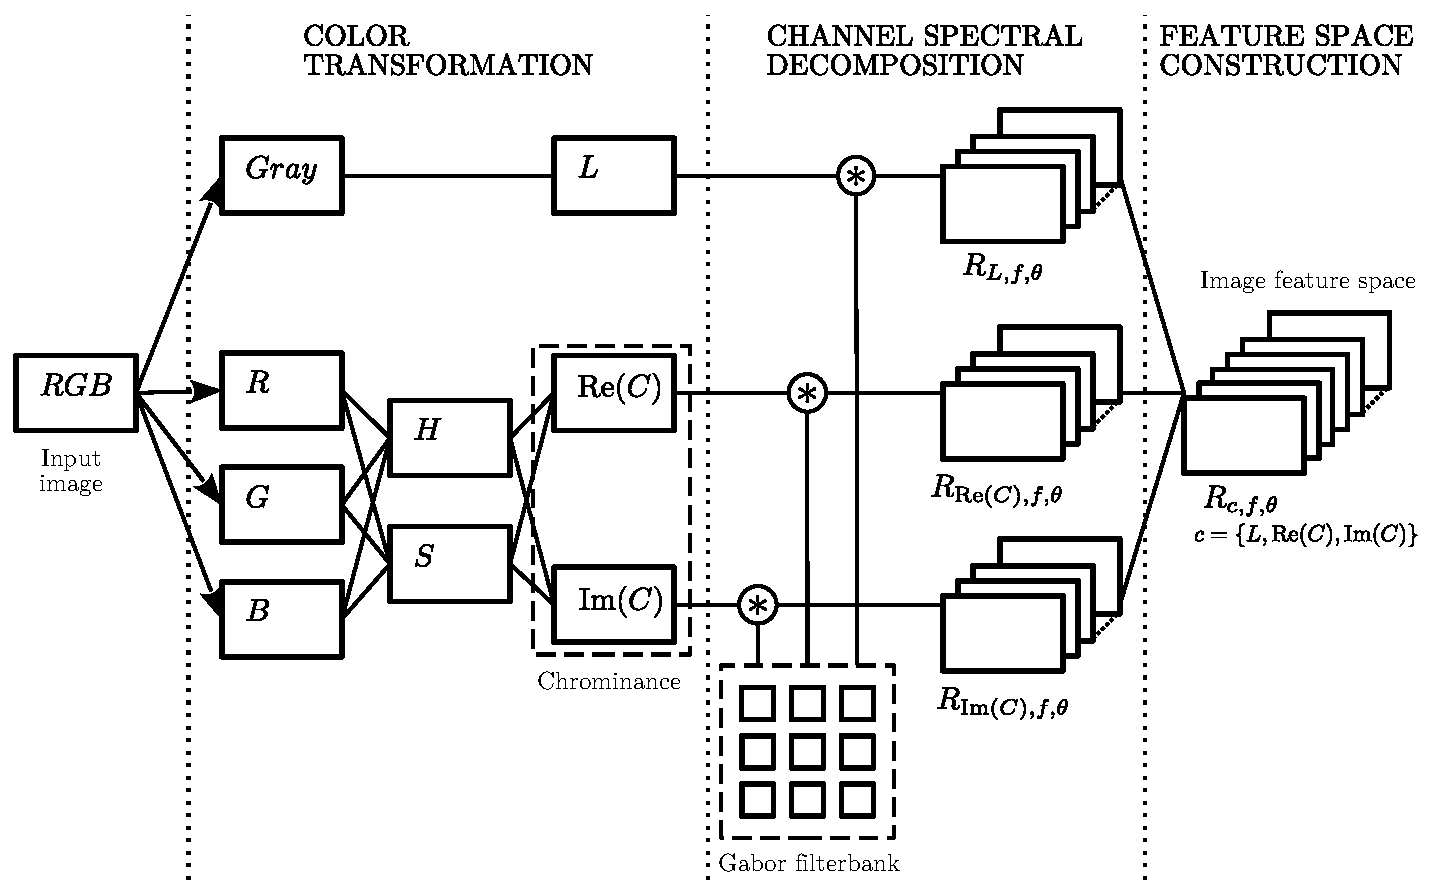
\includegraphics[width=0.5\textwidth]{gabor_color_feature_extraction_diagram}
	\caption{The proposed methodology for the computation of Gabor features in color images.}\label{fig:proposed_pipeline_gabor_feature_extraction}
\end{figure}

\begin{figure}[!ht]
	\centering
	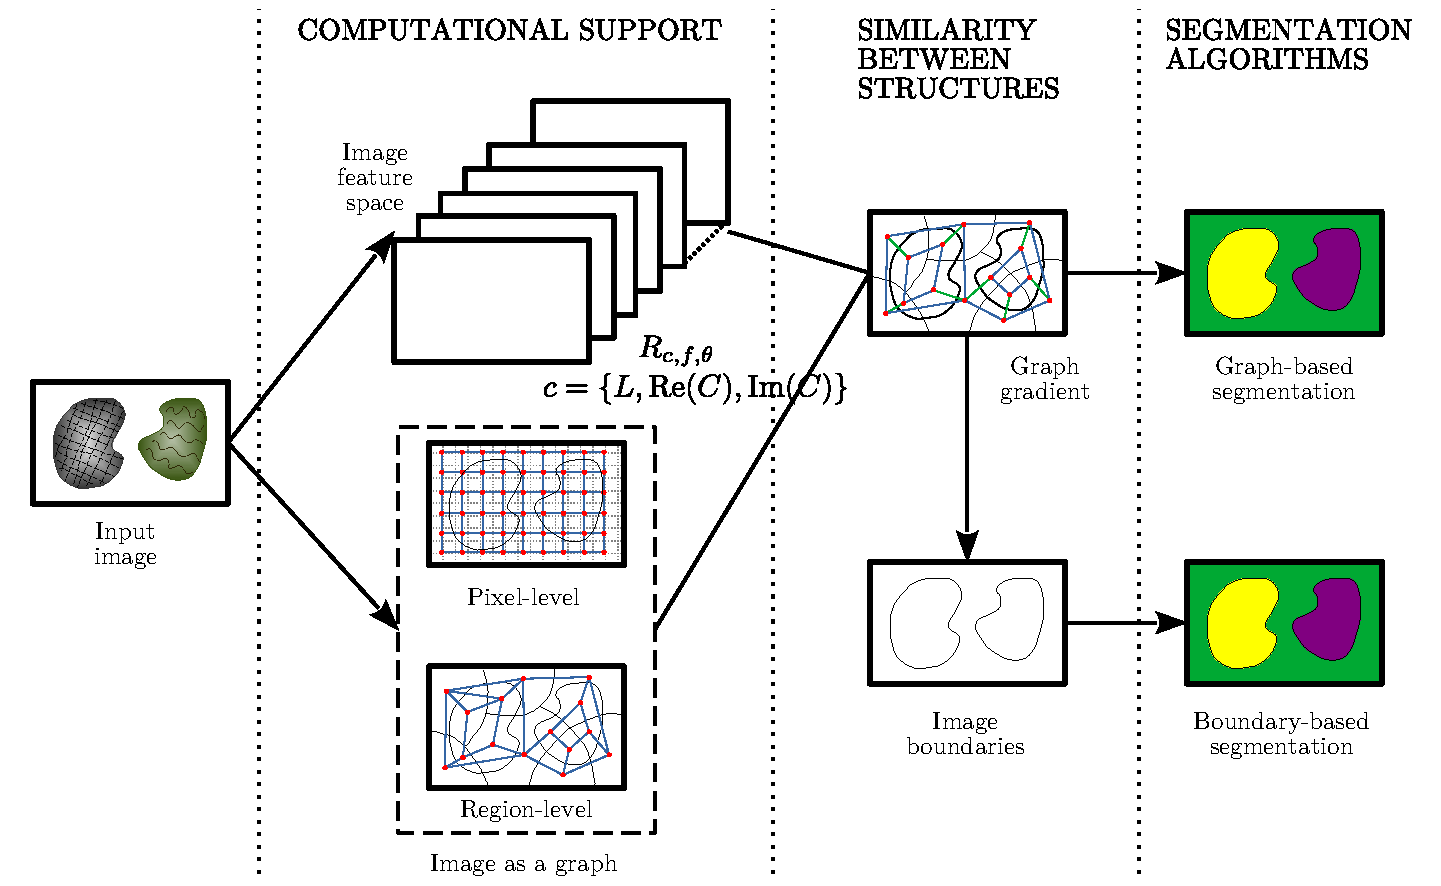
\includegraphics[width=0.5\textwidth]{img_boundaries_segmentation_diagram}
	\caption{General pipeline for extraction of perceptual image boundaries and unsupervised image segmentation.}\label{fig:pipeline_gabor_image_segmentation}
\end{figure}

\section{Related works}

Subsection text here.

% needed in second column of first page if using \IEEEpubid
%\IEEEpubidadjcol

\subsection{Image boundaries}
Edge detection is a fundamental problem of computer vision that has been intensively studied since the early 1970s \cite{Hueckel:JACM:1971, Fram.Deutsch:TC:1975}. The main idea behind traditional approaches to contour extraction is to model edges as discontinuities in the brightness channel of an image. This idea gave way to the creation of mask-based operators such as Sobel \cite{Sobel.Feldman:SAIL:1990}, Roberts \cite{Roberts:Thesis:1963}, Gradient \cite{Maitre:Book:2003} and Prewitt \cite{Prewitt:PPP:1970}, which quantify the presence of an edge through the convolution of a gray level image with local derivative filters. Other techniques, such as Marr and Hildreth \cite{Marr.Hildreth:PRS:1980}, define edges as the zero crossings of the Laplacian of a Gaussian (LoG). The Canny operator \cite{Canny:PAMI:1986} is one of the most popular approaches to this day within traditional methods. This operator follows the same operation principle of the previous methods, adding a non-maximum suppression stage and hysteresis thresholding. 

Despite their efficiency in controlled environments or synthetic images, traditional methods suffer from identifying contours in natural images. The edges of natural images can be present at different scales, and the colors and textures of the scene can generate edges that are perceptually significant to the human eye. Ideally, a contour detection method is intended to simultaneously exploit the brightness, color, and texture properties of an image so that it can handle the boundary perimeters defined by the brightness steps and the regions with consistent color and (or) texture.

One of the relatively recent strategies for identifying perceptual contours is to use the local energy response of an image. The operation principle is simple: generate features from the responses of an image produced by a family of filters at different scales and orientations. The idea has been exploited from different points of view. For example, the use of the Difference of Gaussians (DoG) and its Hilbert transform \cite{Morrone.Owens:PR:1987, Morrone.Burr.ea:RSL:1988} to generate a family of filters. Inspired by Gabor's work, this group of filters comply with the Parseval principle and generate an exact quadrature pair (even and odd symmetry cells). 

The \textit{Probability-of-boundary} (Pb) detector \cite{Malik.Belongie.ea:IJCV:2001} is one of the principal exponents of using a filter bank formed by the DoG and its Hilbert transform. The contour detector only uses the brightness and texture information to obtain the Pb. The brightness information is processed following the intervening contour framework \cite{Leung.Malik:ECCV:1998}, which consists of obtaining the image's quadrature energy, also called oriented energy (OE). The texture information is analyzed using so-called textons \cite{Malik.Belongie.ea:ICCV:1999}. Since each cue (brightness and texture) has a domain of applicability, hence different units of magnitude, they introduce a gating operator based on a neighborhood's texturedness at a pixel. The operator gives, as a result, a local measure that indicates how much two nearby pixels are to belong to the same region. Later in that work, they use spectral graph theory (normalized cut algorithm \cite{JianboShi.Malik:PAMI:2000}) to segment the image into coherent texture and brightness regions. 

This contemporary method, developed by the UC Berkeley research group, was the basis for many other techniques for contour detection and segmentation of natural images widely used today. Most of these works bring substantial improvements to the Pb detector. For example, the seminal papers \cite{Martin.Fowlkes.ea:NIPS:2002} and \cite{Martin.Fowlkes.ea:PAMI:2004} bring together previous works related to Pb and obtain a feature space of four image characteristics: localized OE, Brightness Gradient (BG), Color Gradient (CG), and localized Texture Gradient (TG). To cope with the difference in units of the magnitude of the cues, they use a logistic regression classifier to combine oriented energy, brightness, color, and texture. The proposed supervised method optimizes each feature's weights, formulating it as a two-class classification problem, where they learn the rules for combining cues from the ground truth data of the Berkeley Segmentation Dataset (BSDS) \cite{Martin.Fowlkes.ea:ICCV:2001}.

On the other hand, \cite{Ren:ECCV:2008} showed that the Pb detector improves when using features of the image calculated at different scales. However, a better version of the Pb detector, which has dominated the state of the art scores for several years, is obtained by combining local and global contours \cite{Maire.Arbelaez.ea:CVPR:2008}. The local contours are represented by the multiscale oriented signal mPb, while the global contours are represented by the oriented signal from the spectral partition sPb. The final detector that combines both signals is the globalized Probability-of-boundary gPb, which learns the local and global part's weights through an ascending gradient, taking as reference the BSDS evaluation score.

The Berkeley research group laid the foundation for contour detection and natural image segmentation, providing quantitative comparison methods. However, there are other methods in the literature that use different strategies to calculate image features and detect contours. Such methods can usefully supervise approaches, avoiding the careful hand-drawing of texture and gloss gradients. However, we can also find semi-supervised methods that replace the Pb detector to apply later a pre-processing chain similar to that applied in the Berkeley group methods.

The Berkeley research group laid the foundation for contour detection and natural image segmentation, providing the database and tools for the comparison and quantitative evaluation of the different approaches. Furthermore, Pb has motivated the development of state-of-the-art methods that use different strategies to obtain image features and contour detection. Such methods can use supervised approaches, avoiding careful filter design, computation of texture and brightness gradients, and hand-crafted features. We can also find semi-supervised methods, which generally replace the Pb detector with a supervised detector to apply later a pre-processing chain similar to that applied in the Berkeley group methods to refine the detection.

The set of the most popular supervised methods for contour detection, led by researchers from the University of Pasadena California and colleagues, is based on the calculation of features on channels of integrals of the image \cite{Dollar.Tu.ea:BMVC:2009}. Some examples of these integral channels are image color and gray channels, image responses to linear filters (e.g., Gabor filters, DoG), non-linear image transformations (e.g., Canny edges, gradient magnitude, hysteresis threshold), among others. The calculation of features on the integral channels follows the object detection framework of \cite{Viola.Jones:IJCV:2004}, obtaining first-order and higher-order features such as Haar-like features. Following this principle, a pool of features is obtained by randomly choosing both the integral channel and a rectangle where the features are calculated, allowing the acceleration of the computation of features and boosting learning techniques. 

Some of the supervised edge detectors that use the integral channel features as input are the Boosted Energy Learning (BEL) \cite{Dollar.ZhuowenTu.ea:CVPR:2006}, which attempts to learn an edge classifier in the form of a probabilistic boosting tree from the thousands of simple features calculated in image patches. On the other hand, Sketch tokens \cite{Lim.Zitnick.ea:CVPR:2013} uses the same features as input to a random forest classifier. The peculiarity of this second method is that the classes of the classifier are the so-called sketch tokens; mid-level information patches that represent complex shapes such as joints, corners, vertical and horizontal edges, calculated from the contours of the ground truth. The Structural Edge (SE) detector \cite{Dollar.Zitnick:ICCV:2013} and its different versions \cite{Dollar.Zitnick:PAMI:2015} take these strategies to another level, learning not only the integral input features but also the output space, using structured-output decision forests. The Oriented Edge Forest (OEF) detector \cite{Hallman.Fowlkes:CVPR:2015} outperforms existing supervised methods using a decision forest that analyzes local patches and outputs probability distributions over the space of oriented edges passing through the patch. On the other hand, \cite{Kivinen.Williams.ea:PMLR:2014} propose a fully supervised method (DeepNet) that does not use the framework of the integral features; instead, it calculates complex-cell like covariance features from multiple scales and semantic levels, which depend on the squared response of a filter to the input image. The Object-Contextual Representations (OCR) \cite{Yuan.Chen.ea:arXiv:2021} learns object regions and the relation between each pixel and each object region, augmenting the representation pixels with the object-contextual representation. The Convolutional Oriented Boundaries (COB) \cite{Maninis.Pont-Tuset.ea:ECCV:2016, Maninis.Pont-Tuset.ea:PAMI:2018} produces image contours and region hierarchies starting from generic image classification. Finally, the \cite{Kelm.Rao.ea:CAIP:2019} propose the RefineContourNet, a model based on the ResNet architecture that surpases the state-of-the-art BSDS500 benchmark. 

Another group of approaches to contour detection are those based on sparse local coding. Such techniques are said semi-supervised because they contain two main stages, one unsupervised and the other supervised. The first stage consists of obtaining a generic representation (without information of the contours) from the image's information in an unsupervised way. The second stage consists of transforming the sparse representation of the image into a classification task, wherein the case of contours detection is a two-classes supervised problem to label the pixels as a contour or no contour. Some renowned works under this approach are the detector proposed by \cite{Mairal.Leordeanu.ea:ECCV:2008} and the Sparse Code Gradients (SCG) detector \cite{Ren.Bo:NIPS:2012}. Both works use K-SVD as a dictionary learning algorithm and Orthogonal Matching Pursuit for efficient optimization and sparse coding of each pixel. At the end of the process, they use SVM as a linear classifier on the feature vectors resulting from the reconstruction error with each dictionary for pixel classification. The main difference between these detectors is that the SCG adopts the same scheme as the Pb detector, replacing the brightness, color, and texture gradients with sparse code gradients. Finally, the Sparse Code Transfer (SCT) detector \cite{Maire.Yu.ea:ACCV:2014} improves on the detector of \cite{Mairal.Leordeanu.ea:ECCV:2008} using a larger number of dictionaries at different scales and layers in addition to the multipath sparse coding technique, which rectifies the initial sparse codes to reconstruct the contours with an extra transfer dictionary. The main disadvantage of these semi-supervised methods is the computational time of both processes, dictionary calculation, and learning. 



\subsection{Image segmentation}
There is a fine line between contour detection and image segmentation. In this sense, the Pb contour detector has also influenced image segmentation. The Ultrametric Contour Maps (UCM) \cite{Arbelaez.Maire.ea:PR:2009} uses the gPb to define a measure of dissimilarity (ultrametric distance) between pairs of adjacent regions defined by a hierarchical segmentation operator (HSO). This technique is refined by adding a supplementary pre-processing stage using the oriented watershed transform (OWT), giving rise to the gPb-owt-ucm hierarchical segmentation method \cite{Arbelaez.Maire.ea:PR:2009}. The extensive qualitative and quantitative comparison of these techniques can be consulted in \cite{Arbelaez.Maire.ea:PAMI:2011}.

The Pb contour detector has driven (directly or indirectly) 50 years of research work around perceptual contours detection in natural images and their segmentation. Like the Canny operator, the Pb operator has become a reference work. The importance of this method is that it provides a reasonable basis that considers human perception principles, using operators that have a physical sense. 

\subsection{Bechmark}
We use the benchmark for contour detection and image segmentation of the BSDS. This benchmark uses the precision and recall scores described in chapter \ref{ch:complex_spectral_image_decomposition} (cf. subsection \ref{subsec:quantitative_evaluation}). In addition to these scores, the BSDS benchmark uses the following measures and tools to compare results in contour detection and image segmentation.


\subsubsection{Optimal Dataset Scale (ODS), Optimal Image Scale (OIS)}

A hierarchical segmentation method applied on an image provides a hierarchy $(H, \lambda)$, where the successive ultrametric levels $(\lambda_1, \cdots , \lambda_N )$ correspond to a series of nested segmentations $(S_1, \cdots , S_N )$. To properly evaluate it, one has to compute the score$(S_i , GT )$ for any level $\lambda_i$ of each image's hierarchy. We can then either retain the best $\lambda$-level on the overall dataset, and the corresponding score is the Optimal Dataset Scale (ODS), or retain the best level $\lambda_i$ for each image and average the best individual scores for all images, which correspond to the Optimal Image Scale (OIS). By definition, the ODS is inferior or equal to the OIS. For a gradient image, the levels $\lambda_i$ correspond to the threshold values at which the image contours are evaluated.

\subsubsection{Precision-Recall curve and Average Precision (AP)}

A precision-recall curve (PRC) is a graph that shows the relationship between precision (positive predictive value) in the x-axis, and recall (sensitivity), in the y-axis, for every possible cut-off. The cut-offs for a gradient image are the threshold values at which the image contours are evaluated. Every point on the PRC represents a chosen cut-off; therefore, what we can see in the graph is the precision and the recall we get when choosing a cut-off. The average precision (AP) on the full recall range is equivalent to the area under the precision-recall curve.

\subsubsection{Segmentation Covering (SC)}

The Segmentation Covering is a measure introduced by \cite{Arbelaez.Maire.ea:PR:2009} that we can see as the generalization of the classic overlap measure between two regions $R$ and $R'$ defined as
\begin{equation}
	O(R, R') = \frac{R \cap R'}{R \cup R'}
\end{equation}

The Segmentation Covering (SC) extends the overlap measure so that the covering of a segmentation $S$ by a segmentation $S'$ is defined as 
\begin{equation}
	SC(S' \rightarrow S) = \frac{1}{N}\sum_{R \in S} |R| \cdot \underset{R' \in S'}{\mathrm{max}} O(R, R')
\end{equation}
where $N$ denotes the total number of pixels in the image and $\mathcal{O}$ denotes the overlap between two regions $R$ and $R'$.

In the case of a family of multiple image ground-truth segmentations $\{GT_i\}$ f, the covering of a machine segmentation $S$ is defined by first covering $S$ individually for each human segmentation $GT_i$, and then averaging over the different humans. If the machine segmentation explains all of the human data, it achieves a perfect covering score.

\subsubsection{Probabilistic Rand Index (PRI)}
The Rand Index has initially been introduced for clusterings evaluation. It operates by comparing the compatibility of assignments between pairs of points in the compared clusters. The Rand Index between a machine segmentation $S$ and a ground-truth $GT$ is the sum of the number of pixels pairs with the same labels in $S$ and $GT$, and of those with different labels in the two segmentations, divided by the total number of pixels pairs. The Probabilistic Rand Index (PRI) \cite{Unnikrishnan.Pantofaru.ea:CVPR:2005} is a variant introduced for the case when multiple ground truths are available. If we consider a set of ground-truth segmentations $\{GT_k\}$, the PRI is given by:
\begin{equation}
	PRI(S, \{GT_k\}) = \frac{1}{T}\sum_{i<j} [c_{ij}p_{ij} + (1-c_{ij})(1-p_{ij})]
\end{equation}
where $c_{ij}$ is the event the pixels $i$ and $j$ have the same label and $p_{ij}$ its probability. $T$ is the total number of pixel pairs.

\subsubsection{Variation of Information(VI)}
The Variation of Information (VI) is also a measure that has been introduced to compare clusterings \cite{Meila:LTKM:2003}. It measures the distance between two segmentations relatively to their average conditional entropies given by:
\begin{equation}
	VI(S, S') = H(S) + H(S') - 2I(S, S')
\end{equation}
where $H$ and $I$ respectively represent the entropies and mutual information between two data clusterings $S$ and $S'$. In our case, these clusterings are the test and ground-truth segmentations.


\section{Gabor Filters for Full Image Spectrum Coverage}
%Optimal Gabor filters
%The Gabor Filter as a Measurement Tool

This section presents a reminder of the signal theory applied to image processing for feature extraction. First, we show the reasons for restricting signal analysis in two predefined domains: time and frequency (for the 1-d case) and space and frequency (for the 2-d case). We especially recall Gabor filter theory and properties by showing how these filters are related to Heisenberg's uncertainty principle.

As we mentioned before, we use Gabor filters as a tool to measure the information that characterizes a signal. Since the signal carries relevant information at different points and scales (either in the spatial or space-frequency domain), a well-known strategy used in the literature is to create a filter bank that covers most of the spectrum to be able to reconstruct the original signal.

\subsection{Signals in Two Domains}
Bound by the Fourier transform, there are two equivalent representations of a signal (one-dimensional (1-d) or two-dimensional (2-d)). The first represents the signal as a function of time, while the second represents it as a function of frequency. These two representations carry the same information but in different ways; besides, we can go from one to another via the Fourier transform (or the inverse Fourier transform), making these special interest descriptions. We define the pair of 1-d Fourier transforms (FT) as follows
\begin{equation}\label{eq:fourier_transforms_1d}
    \begin{gathered}
        H(\upsilon) = \mathcal{F}\{h(t)\} = \int_{-\infty}^{\infty} h(t) e^{-j2\pi f t} dt \\
        h(t) = \mathcal{F}^{-1}\{H(\upsilon)\} = \int_{-\infty}^{\infty} H(\upsilon) e^{j2\pi f t} df 
    \end{gathered}
\end{equation}
while for the 2-d case, we define the FT as

\begin{equation}\label{eq:fourier_transforms_2d}
    \begin{gathered}
        H(u, v) = \mathcal{F}\{h(x, y)\} = \int_{-\infty}^{\infty} \int_{-\infty}^{\infty} h(x, y) e^{-j2\pi (ux + vy)} dx dy \\
        h(x, y) = \mathcal{F}^{-1}\{H(u, v)\} = \int_{-\infty}^{\infty} \int_{-\infty}^{\infty}  H(u, v) e^{j2\pi (ux + vy)} du dv 
    \end{gathered}
\end{equation}

%Both representations of the signal are somewhat ideal since the first operate at defined instants of time while the second operates on an infinite series of successive waves at defined frequencies \cite{Gabor:JIEE:1946}. 

It is evident that the function $h(t)$ (resp. $h(x, y)$) is located in both domains; however, it is also well known that no signal with compact support can have a finite Fourier transform and vice versa \cite{Bracewell:FourierBook:1999}, there is a particular uncertainty in the time and frequency locations of $h(t)$ (resp. space and frequency locations of $h(x, y)$).

This is the mathematical statement of the uncertainty principle in signal processing \cite{Petrou.Sevilla:Book:2006}.

\subsection{1-d Gabor Filters}
The uncertainty principle shows that time and frequency are two fundamental domains and physically measurable quantities, but still idealizations if we consider one from the other's perspective. Frequency is a simple waveform in the time domain, but to be sharply defined in the frequency domain, it must be infinite in the time domain, i.e., a waveform that has always existed and will remain forever. In everyday life, it is complicated to find phenomena with these characteristics; it is more common to find signals that have properties from both domains; certainly, they have some frequency characteristics, but they also have a starting point, and after some time, these signals begin to fade away. This phenomenon motivated Dennis Gabor to represent signals simultaneously in time and frequency through the Gabor Elementary Function (GEF) \cite{Gabor:JIEE:1946}. The function represents the minimal quantum of information, i.e., the minimal amount of simultaneous information in time and frequency. In other words, it occupies the minimal area, given by a rectangle, in the time-frequency plane.  
%(see appendix \ref{ch:uncertainty_principle})

The Gabor function is derived form the uncertainty principle, therefore, it has a shape for which the product $\Delta t \Delta \upsilon$ assumes the smallest possible value. In other words, the Gabor function is the one that transforms inequality of Eq. \eqref{eq:uncertainty_principle_freq} into the equality $\Delta t \Delta \upsilon = \frac{1}{4 \pi}$. Then, the Gabor function is defined as the modulation product of a harmonic oscillation (a sinusoidal wave) of any frequency with a pulse of the form of a probability function (a Gaussian function) \cite{Gabor:JIEE:1946} and is represented as
\begin{equation}\label{eq:gabor_function_1d_time}
    g(t) =  e ^{-\alpha^2(t-t_0)^2} e ^{j 2 \pi f t + \phi}
\end{equation}
where $\alpha$ express the \textit{spread} and $t_0$ denotes the centroid of the Gaussian function, $f$ is the frequency of the sinusoidal wave, and $\phi$ defines the phase shift of the oscillation.

The Fourier transform of Eq. \eqref{eq:gabor_function_1d_time} defines the representation of the Gabor function in the frequency domain $G(\upsilon) = \mathcal{F}\{g(t)\}$ with the following analytical form

\begin{equation}\label{eq:gabor_function_1d_freq}
    G(\upsilon) =  \sqrt{\frac{\pi}{\alpha^2}} e ^{-\left(\frac{\pi}{\alpha}\right) ^{2} (\upsilon-f)^2} e ^{-j 2 \pi t_0 (\upsilon-f) + \phi}
\end{equation}

The equations \eqref{eq:gabor_function_1d_time} and \eqref{eq:gabor_function_1d_freq} show straightforward that the center of gravity $t_0$ is equal to \eqref{eq:center_of_gravity} and the spectral center of gravity $f$ is equal to \eqref{eq:spectral_center_of_gravity}, i.e., the Gabor functions follow Heisenberg's uncertainty principle.   

\begin{figure}[!ht] 

	\centering
	\begin{subfigure}[t]{\dimexpr0.45\textwidth+20pt\relax}
    	\makebox[20pt]{\raisebox{40pt} {\captext{(a)}} }%
    	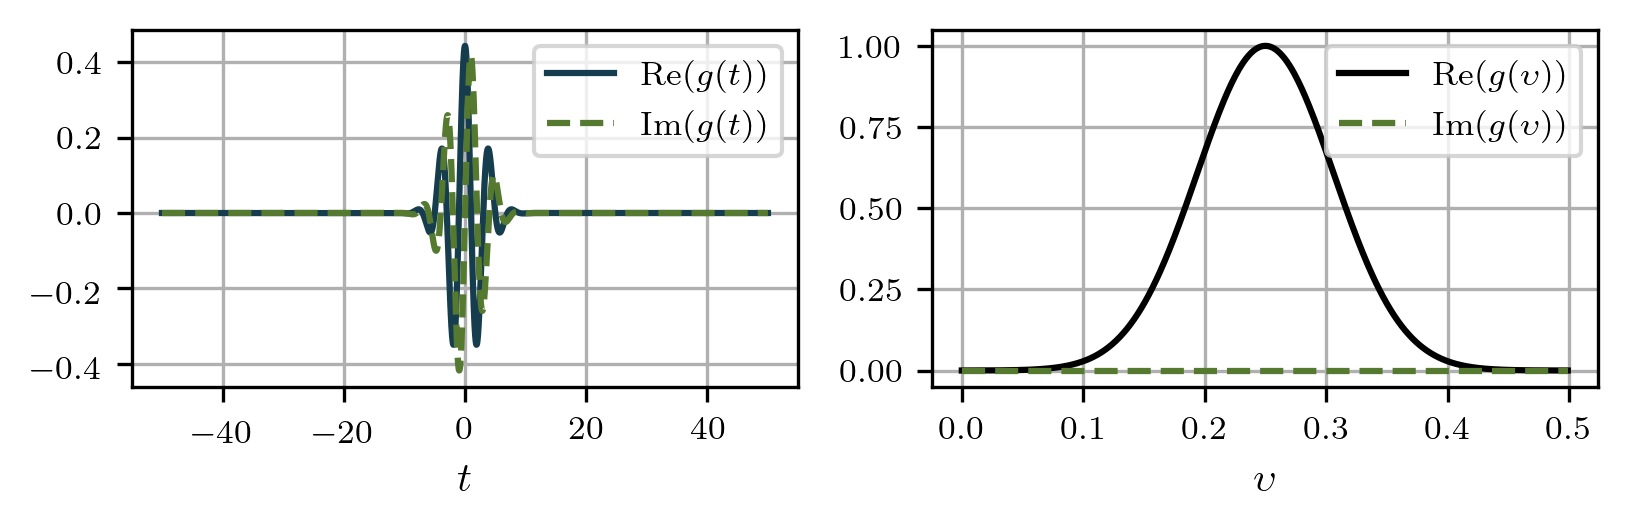
\includegraphics[width=\dimexpr\linewidth-20pt\relax]{1D_GaborFilter_hor_f4_g1}
    \end{subfigure}\vspace{-1em}
	\begin{subfigure}[t]{\dimexpr0.45\textwidth+20pt\relax}
    	\makebox[20pt]{\raisebox{40pt} {\captext{(b)}} }%
    	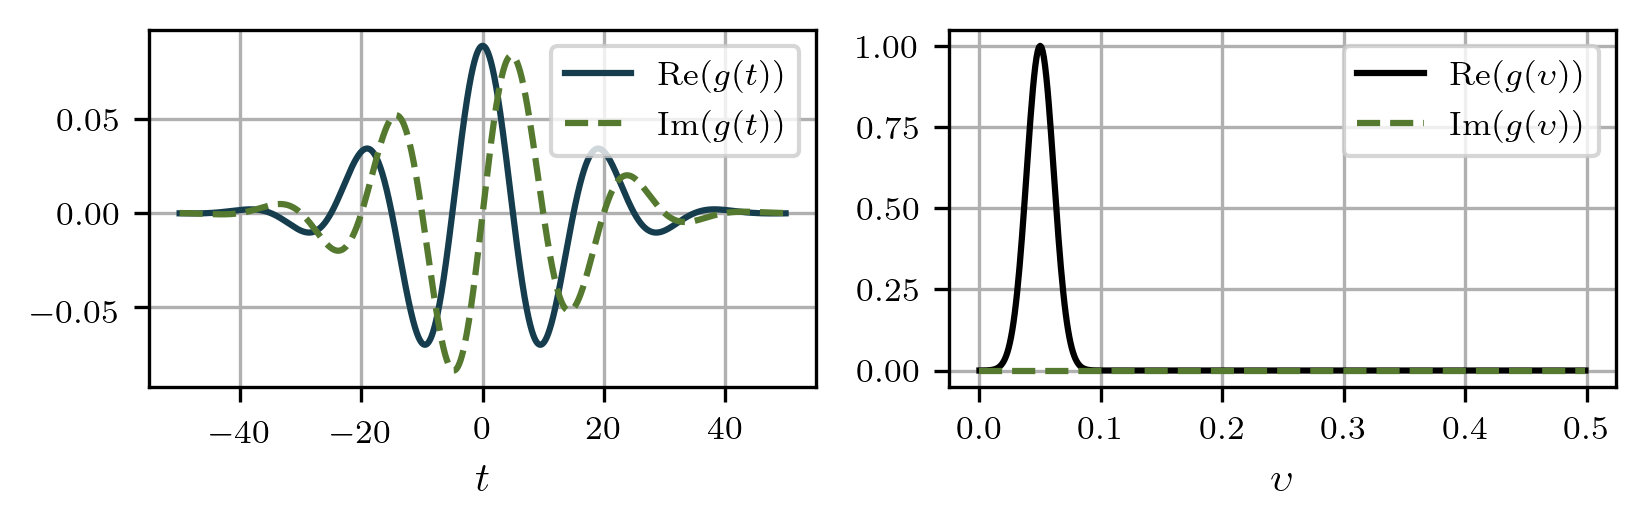
\includegraphics[width=\dimexpr\linewidth-20pt\relax]{1D_GaborFilter_hor_f20_g1}
    \end{subfigure}\vspace{-1em}
	\begin{subfigure}[t]{\dimexpr0.45\textwidth+20pt\relax}
    	\makebox[20pt]{\raisebox{40pt} {\captext{(c)}} }%
    	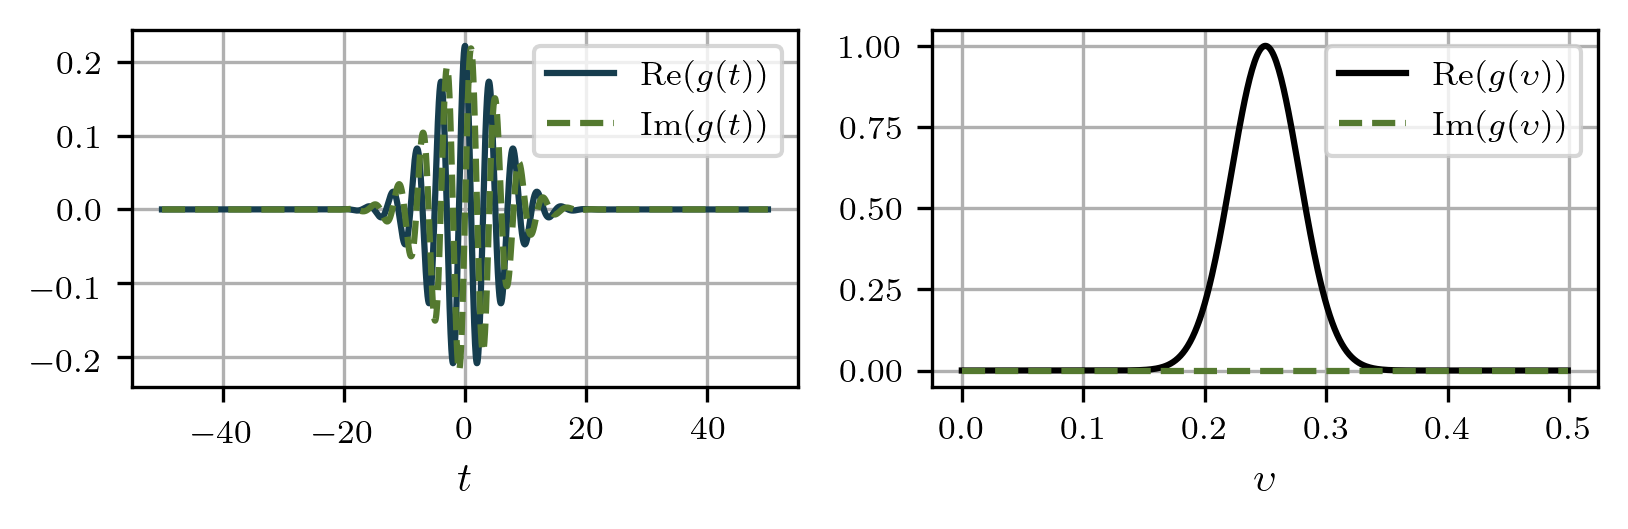
\includegraphics[width=\dimexpr\linewidth-20pt\relax]{1D_GaborFilter_hor_f4_g2}
    \end{subfigure}\vspace{-1em}
	\begin{subfigure}[t]{\dimexpr0.45\textwidth+20pt\relax}
    	\makebox[20pt]{\raisebox{40pt} {\captext{(d)}} }%
    	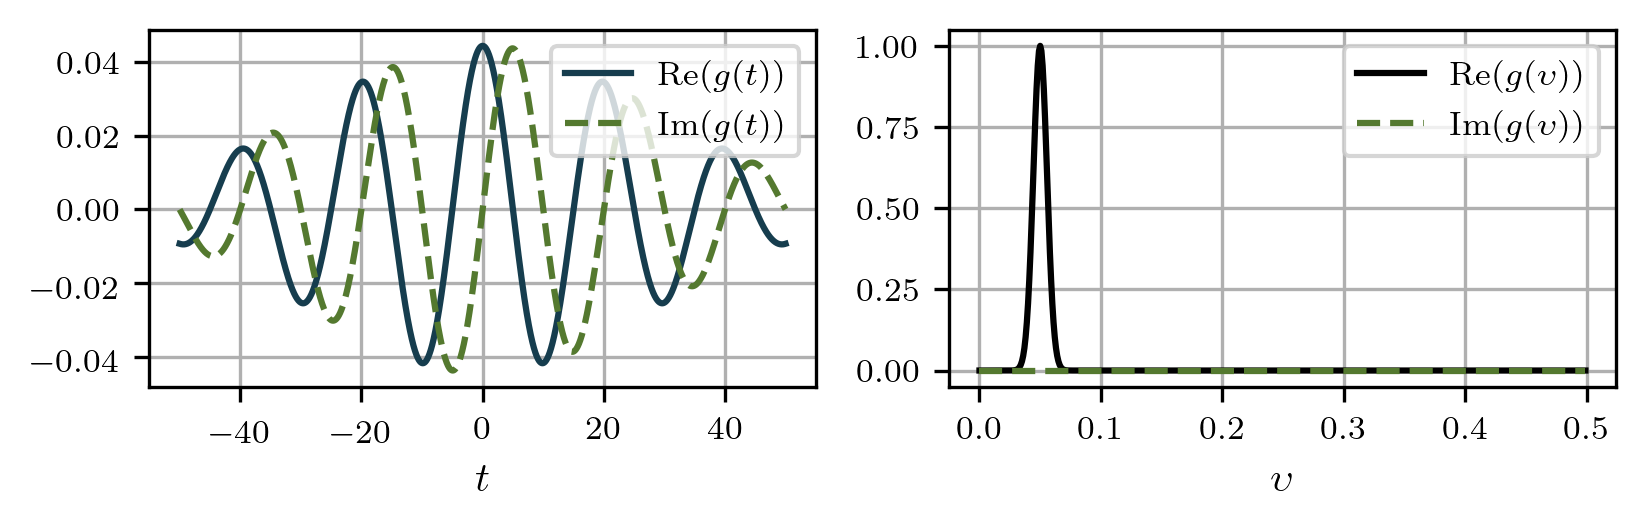
\includegraphics[width=\dimexpr\linewidth-20pt\relax]{1D_GaborFilter_hor_f20_g2}
    \end{subfigure}\vspace{-1em}
	
  	\caption{Visualization of the uncertainty principle in 1-d Gabor filters. First column: filters on the time domain, Second column: filters on the frequency domain. \captext{(a)} $f = 1/4$, $\gamma = 1$; \captext{(b)} $f = 1/20$, $\gamma = 1$; \captext{(c)} $f = 1/4$, $\gamma = 2$; \captext{(d)} $f = 1/20$, $\gamma = 2$.}
  \label{fig:examples_1D_GaborFilter}
\end{figure}

\subsubsection{Filter normalization} \label{subsec:filter_normalization}
We can define the Gabor filter more appropriately by taking the following justifications. First, we must remember that we use the Gabor function as a linear filter to analyze a signal. Under this condition, the temporal analysis of the signal is carried out using the convolution operator. Considering that the Gabor function is concentrated near the time instant $t_0$ and that a convolution centered at the origin is preferable, we consider $t_0 = 0$. Since there is no evidence that any specific phase would be more beneficial than any other, another parameter that we can omit is the phase shift $\phi$. Moreover, for the functions to be similar at all locations, the phase shift should depend on the location $t_0$, and thus, the phase shift can be removed from the origin-centered filter ($\phi$ = 0). Then, the Gabor filter function in its compact form is defined as 

\begin{equation}\label{eq:gabor_function_1d_timefreq_compact}
    \begin{gathered}
         g(t) =  e ^{-\alpha^2 t^2} e ^{j 2 \pi f t } \\
         G(\upsilon) =  \sqrt{\frac{\pi}{\alpha^2}} e ^{-\left(\frac{\pi}{\alpha}\right) ^{2} (\upsilon-f)^2} 
     \end{gathered}
\end{equation}

We can normalize the Gabor filter depending on the application we will use it. However, in this thesis, we use the general normalization based on the multi-domain representation property of the function following the subsequent conditions \cite{Boukerroui.Noble.ea:JMIV:2004}:

\begin{enumerate}
    \item Maximum condition:
        \begin{equation}\label{eq:maximun_condition}
            \max{|G(\upsilon)|} = 1
        \end{equation}
    \item Constant spectra condition:
        \begin{equation}\label{eq:constant_spectrum_condition}
            \int_{-\infty}^{\infty} |g(t)| dt = 1
        \end{equation}        
\end{enumerate}

From the equation \eqref{eq:gabor_function_1d_freq}, it is evident that the maximum response of the Gabor filter in the frequency domain is a function of $\sqrt{\pi/\alpha^2}$, therefore, its inverse
\begin{equation}\label{eq:normalization_factor}
    \sqrt{\frac{\alpha^2}{\pi}}
\end{equation}
can be used as the normalization factor in the time domain to fulfill the two conditions mentioned above. Then using the normalization factor \eqref{eq:normalization_factor}, the normalized Gabor filter is defined as

\begin{equation}\label{eq:gabor_function_1d_timefreq_normalized}
    \begin{gathered}
         g(t) =  \sqrt{\frac{\alpha^2}{\pi}} e ^{-\alpha^2 t^2} e ^{j 2 \pi f t } \\
         G(\upsilon) =  e ^{-\left(\frac{\pi}{\alpha}\right) ^2 (\upsilon-f)^2}
     \end{gathered}
\end{equation}

\begin{figure}[!ht]
	\centering
	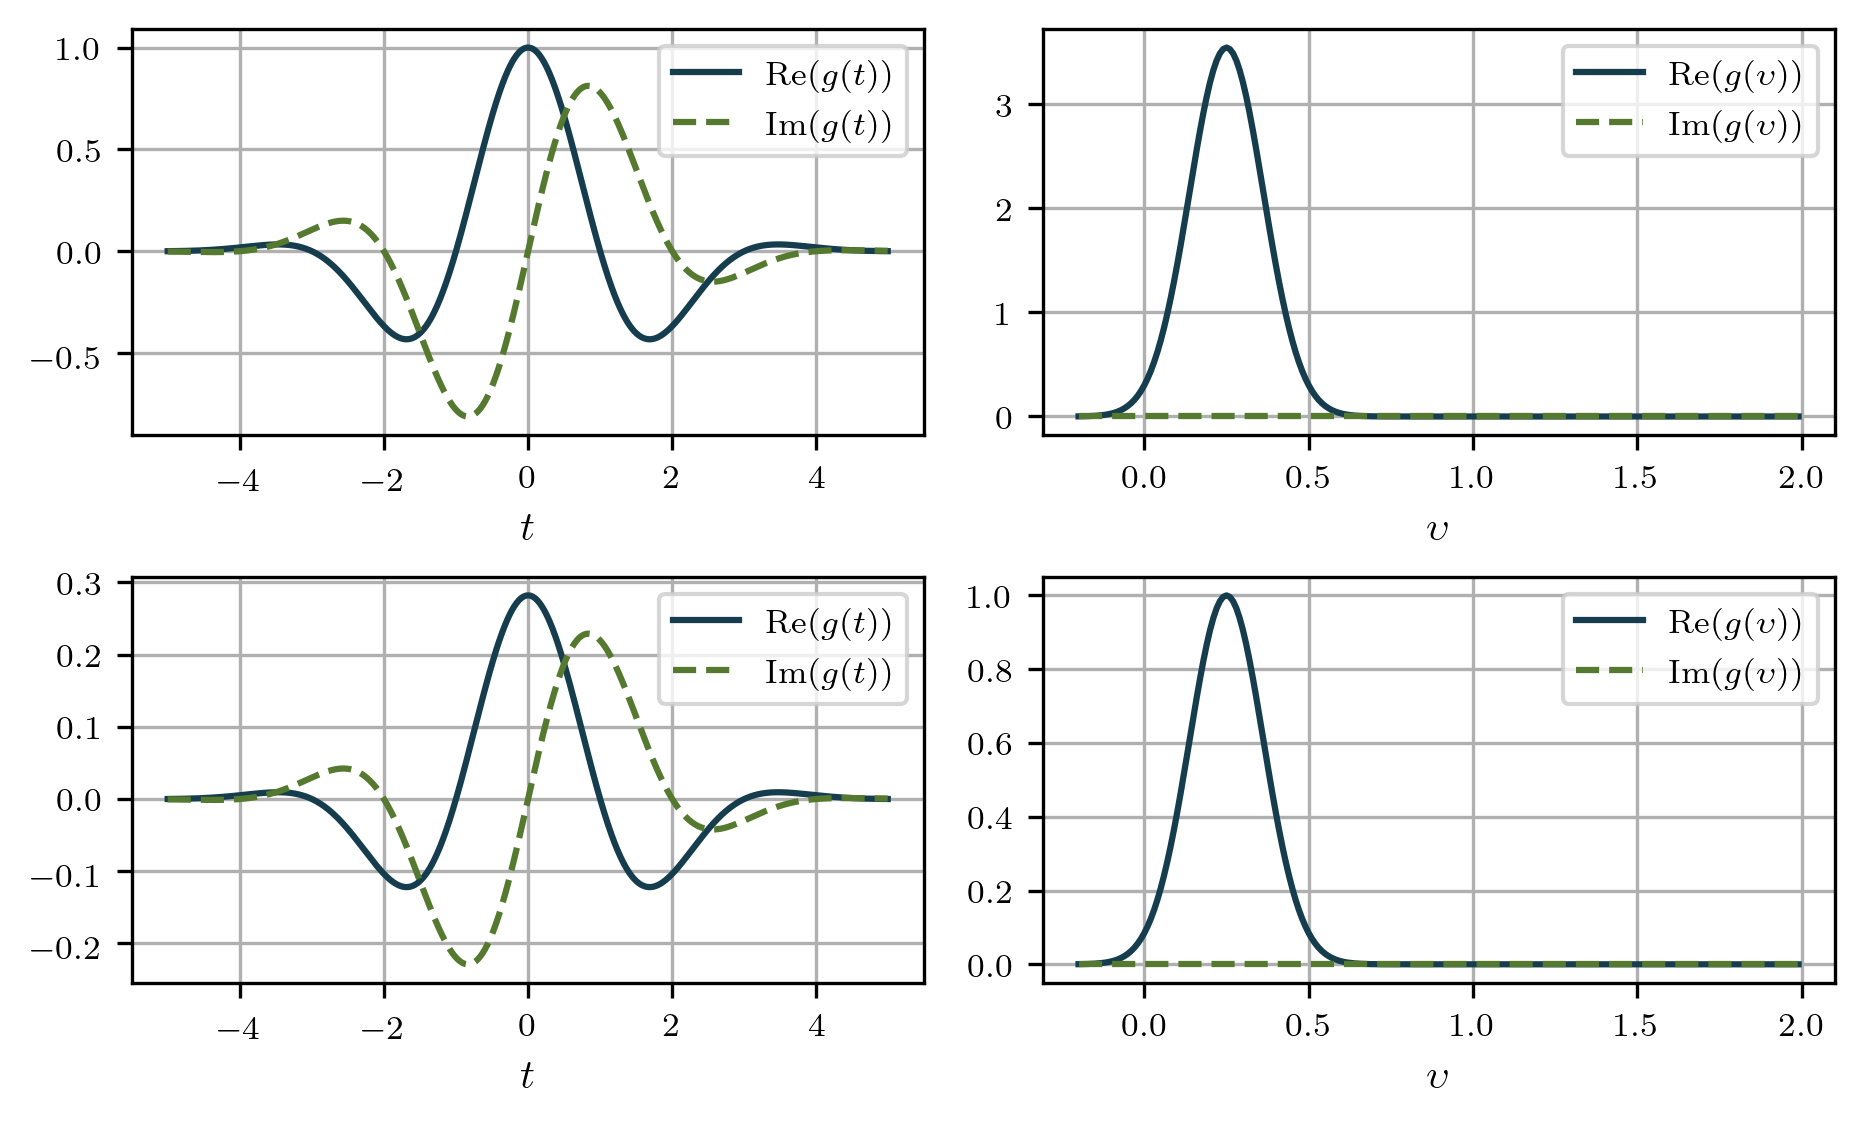
\includegraphics[width=0.45\textwidth]{GaborFilter_timefreq_1d_norm_efect}
	\caption{1-d Gabor filter in the time domain (first column) and in the frequency domain (second  column). From top to bottom: non-normalized and normalized Gabor filter with [$f =1/4$, $\alpha=0.5$, $t_0=0$].}\label{fig:GaborFilter_timefreq_norm_efect}
\end{figure}

Figure \ref{fig:GaborFilter_timefreq_norm_efect} shows a Gabor filter in the time and frequency domain before and after normalization following the two conditions described above. At this point, it is important to note that normalization is an essential step in the multi-spectral analysis and the feature extraction of a signal.

\subsubsection{Frequency filter spacing}\label{subsec:frequency_filter_spacing}
Our main interest in Gabor filters is the multi-spectral analysis of a function. We accomplish this by using multiple Gabor functions as filters that are tuned on several frequencies $f_m$. This group of filters is known as a \textit{Gabor filter bank}. The separation between the filter bank is defined through the half-response spatial frequency bandwidth $B_F$ measured between two central frequencies $f_1 < f_2$ \cite{Granlund:CGIP:1978}. This bandwidth is measured in octaves and we can express it as
\begin{equation}\label{eq:octave_spacing}
    B_f = \log_2 \left( \frac{f_2}{f_1} \right)
\end{equation}

The frequency bandwidth eq. \eqref{eq:octave_spacing} shows that the central frequencies $f_m$ must have a logarithmic relationship to maintain a homogeneous spacing between the filters. The scaling factor $k=2^{B_F}$ gives the logarithmic relationship, so the frequency of each filter ($f$) in this case corresponds to the scale information. Then we can write the central frequencies as
\begin{equation}
	f_m = k^{-m} f_{max}\textrm{,} \quad m = \{1, \cdots, M\} \label{eq:filterbank_frequencies}
\end{equation} 
where $f_m$ is the $m$th frequency, $f_{max}$ is the maximum desired frequency, $k>1$ is the frequency scaling factor, and $M$ is the total number of frequencies of the filter bank.

The octave spacing between two adjacent filters is an interesting property of the Gabor filters; however, the filters denoted by the Eqs. \eqref{eq:gabor_function_1d_timefreq_normalized} have a spread that only depends on the parameter $\alpha$, regardless of its central frequency $f$. This trait means that when implementing the Gabor function in a filter bank at different frequencies to obtain a multi-spectral decomposition of a signal, all of the filters will have the same spread in the frequency domain. We can see this effect in figure \ref{fig:filterbnk_octave_spacing}, where we show a filter bank with five central frequencies and an adjacent filter's spacing of one octave, that is, $M=5$ and $B_F = 1$. 


\subsubsection{Frequency crossing point}
The fact we choose the filter bank's central frequencies $f_m$ to have a constant separation causes two adjacent Gabor functions to intersect at a particular point on the frequency axis. For example, in a filter bank formed with two Gabor functions with central frequencies $f_1$ and $f_2$, the low cut-off frequency of the function at $f_1$ coincides with the high cut-off frequency of the function at $f_2$. Generally, in the literature, the crossing point $c_1$, corresponds to the points where the Gabor function has decreased half of its maximum value, i.e., $c_1= 1/2=0.5$ \cite{Granlund:CGIP:1978}. However, by setting the crossing point to half of the maximum value, the filter bank does not cover the input signal's entire spectrum. Consequently, the filter bank will not respond (or the response will be minimal) to artifacts oscillating between central frequencies.

We obtain the mathematical expression of this crossing point $c_1$ by defining a frequency interval $\Delta f$, representing the distance between points where the function $G(\upsilon)$ begins to decrease. The Gabor function has a peculiarity;  its analytical form in the frequency domain is completely defined by the Fourier transform of the normalized Gaussian function Eq. \eqref{eq:gabor_function_1d_timefreq_normalized}.

\begin{equation}\label{eq:1d_gaussian_function_freq}
    G(\upsilon) = w(\upsilon) = e ^{-\left(\frac{\pi}{\alpha}\right) ^{2} (\upsilon-f)^2}
\end{equation}
therefore, evaluating eq. \eqref{eq:1d_gaussian_function_freq} at $\upsilon = f + \frac{\Delta f}{2}$
\begin{equation}\label{eq:constant_crossing_point}
    G\left(f + \frac{\Delta f}{2}\right) = e^{-\left(\frac{\pi}{\alpha}\right)^2 \left(\frac{\Delta f}{2}\right)^2} = c_1 G(f) 
\end{equation}
we obtain the expression of the half-frequency interval 
\begin{equation}\label{eq:frequency_interval_crossing_point}
    \frac{\Delta f}{2} = \frac{\alpha}{\pi}\sqrt{\ln \left(\frac{1}{c_1}\right)}
\end{equation}
from which we obtain that the crossing point is defined as
\begin{equation}\label{eq:crossing_point}
    c_1 = e^{-\left(\frac{\alpha}{\pi} \right)^2 \left(\frac{\Delta f}{2}\right)^2 }
\end{equation}

This expression allows us to control the intersection point of two adjacent filters of the filter bank. Modifying the crossing point allows the generation of filter banks that cover (almost) the entire frequency spectrum, translating into a more faithful decomposition of the input signal.

\begin{figure}[!ht]
\centering
    \subcaptionbox{\label{fig:filterbnk_octave_spacing}}{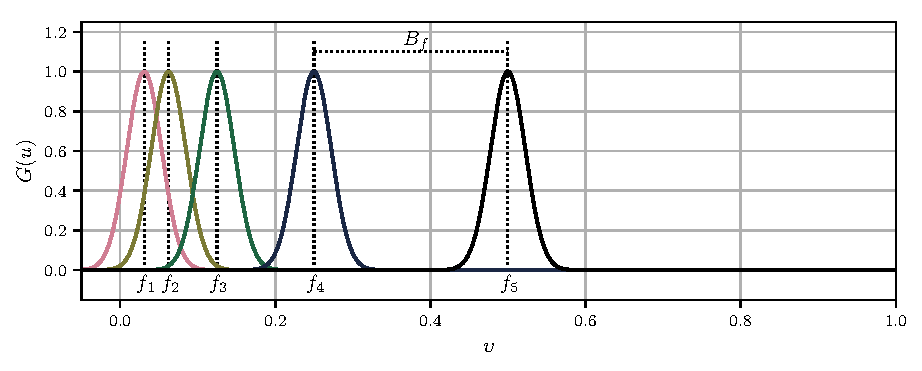
\includegraphics[width=0.5\textwidth]{GaborFilterbank_freq_1d_octave_spacing.pdf}} \\
    \subcaptionbox{\label{fig:filterbnk_half_crossingpoint}}{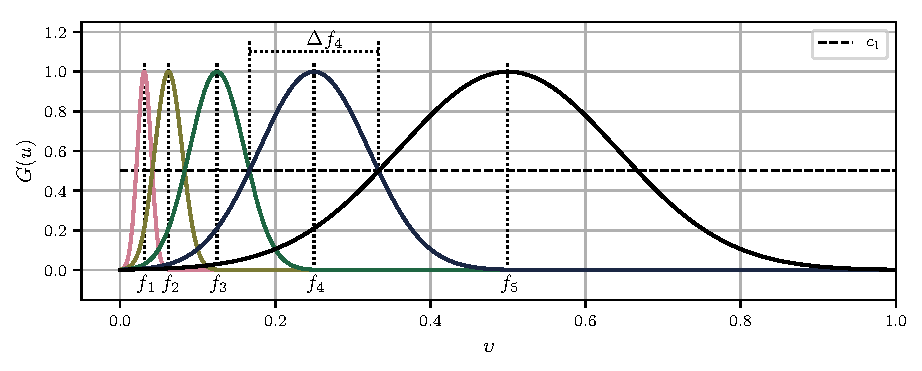
\includegraphics[width=0.5\textwidth]{GaborFilterbank_freq_1d_half_crossingpoint.pdf}}\\
    \subcaptionbox{\label{fig:filterbnk_new_crossingpoint}}{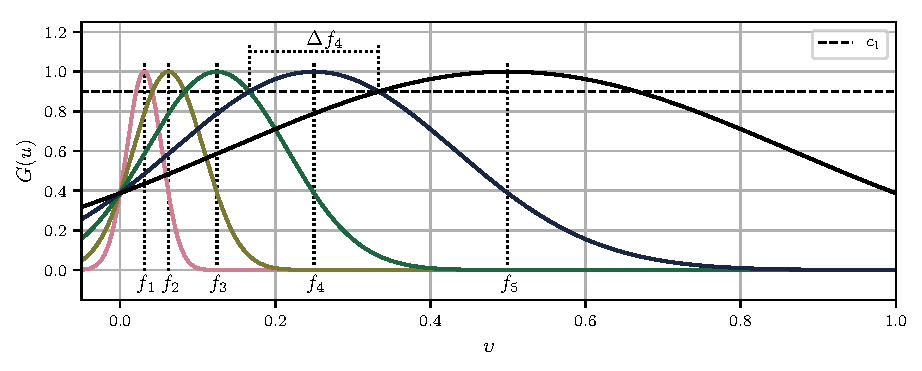
\includegraphics[width=0.5\textwidth]{GaborFilterbank_freq_1d_new_crossingpoint.pdf}}
\caption{Filter spacing and crossing point effect represented on a bank of filters in the frequency domain: \captext{(a)} Separation of filters in octaves without crossing point between adjacent filters $[B_F=1, \alpha=0.1, c_1=-]$, \captext{(b)} High and low cut-off frequency points given by $\Delta f$ $[B_F=1, \alpha=f/\gamma, c_1=0.5]$, \captext{(c)} Filter bank behavior after changing the crossing point $[B_F=1, \alpha=f/\gamma, c_1=0.9]$.}\label{fig:1d_filterbank_spacing}
\end{figure}


\subsubsection{Effective and Adaptable Gaussian Envelope}
The full bandwidth $B_F$ (expressed in octaves) of a Gabor filter with center frequency $f$ and cut-off frequency interval $\Delta f$ is defined as \cite{Daugman:JOSA:1985}.
\begin{equation}\label{eq:frequency_bandwidth_interval}
    B_F = \log_2 \left( \frac{f + \frac{\Delta f}{2} }{f - \frac{\Delta f}{2}} \right)
\end{equation}

It is clear that using the half-frequency interval Eq. \eqref{eq:frequency_interval_crossing_point} into the frequency bandwidth Eq. \eqref{eq:frequency_bandwidth_interval}, we find an expression that introduces a relationship between the frequency bandwidth $B_F$, the central frequency $f$, and the spread of the Gabor filter $\alpha$.
\begin{equation}\label{eq:frequency_bandwidth}
    B_F = \log_2 \left( \frac{ \frac{f}{\alpha} \pi + \sqrt{\ln \left(\frac{1}{c_1}\right)} }{ \frac{f}{\alpha} \pi - \sqrt{\ln \left(\frac{1}{c_1}\right)} } \right)
\end{equation}
The relationship is noticeable through the ratio 
\begin{equation}\label{eq:gamma_ratio}
    \gamma = \frac{f}{\alpha}
\end{equation}

The ratio given in Eq. \ref{eq:gamma_ratio} allows generating Gabor filters of variable size as a function of the center frequency. For this, we must remember that the window size of a Gabor function is denoted by the effective width of a Gaussian function, which in the time domain has a form of
\begin{equation}\label{eq:1d_gaussian_function_time}
    w(t)=e^{-\frac{(t-t_0)^2}{2\sigma^2}}
\end{equation}

The Gaussian window Eq. \ref{eq:1d_gaussian_function_time} is infinite in its extent, so it is characterized by its locality $t_0$ and standard deviation $\sigma$, implicit in the Gabor function parameter $\alpha$ as $\alpha^2 = 1 / 2 \sigma^2$. By setting the standard deviation dependent on the frequency ratio and the central frequency, we find that
\begin{equation}
	\sigma = \frac{\gamma}{\sqrt{2}f} \label{eq:1D_Gaussian_envelope_width}
\end{equation} 
makes the Gabor's window adaptive as a function of the frequency.

In addition to adapting the filter size, with Eq. \eqref{eq:1D_Gaussian_envelope_width}, we make the Gabor filter effective; that is, we make the filter envelope correspond to the time (resp. spatial) support where the function's values are significant. We use the empirical \textit{three-sigma} rule \cite{Pukelsheim:AMSTAT:1994}, a conventional heuristic that expresses that nearly $99.7\%$ of the Gaussian distribution's energy lies within three standard deviations of the mean. Therefore, we define the shortest interval of the function that includes most of the energy as 
\begin{equation}
	\kappa = \lbrace p ~|~ x \in [-3\sigma, 3\sigma] \rbrace \label{eq:1D_gabor_support}
\end{equation}

The fact that the bank filters have the same width at all frequencies is not a problem, nor is it a requirement to analyze a signal with the Gabor function. However, making the filter width dependent on its frequency implies a multi-resolution analysis since the filters behave like a scaled version of each other. The advantages of an effective adaptative envelope are related to the computation time and the loss of information when we filter a signal with a Gabor filterbank. Figure \ref{fig:1D_space_Gaborfilterbank} illustrates the advantages of using a filter bank with adaptive and effective support (Fig. \ref{fig:1D_space_Gaborfilterbank_env}) versus a conventional filter bank (Fig. \ref{fig:1D_space_Gaborfilterbank_wo_env}). More precisely, in the case of constant envelope width, for the example $\kappa = \lbrace p ~|~ x \in [-50, 50] \rbrace$ (see Fig. \ref{fig:1D_space_Gaborfilterbank_wo_env}), the computation time of the responses is the same for all filter frequencies. In contrast, with the adaptive envelope, the calculation time is reduced for high frequencies since the envelope width is smaller (compare images on the first column of Fig. \ref{fig:1D_space_Gaborfilterbank}). Moreover, there is a risk of losing information from the original signal if the chosen envelope is not large enough for low frequencies to fit in(compare images on the last column of fig. \ref{fig:1D_space_Gaborfilterbank}). Using the adaptative and effective envelope width, we recover as much energy as possible from the signal by optimizing the response's computation time for each frequency $f$ of the filter.

\begin{figure}[!ht] 
	\centering
	\begin{subfigure}[b]{0.22\textwidth}
		\centering
		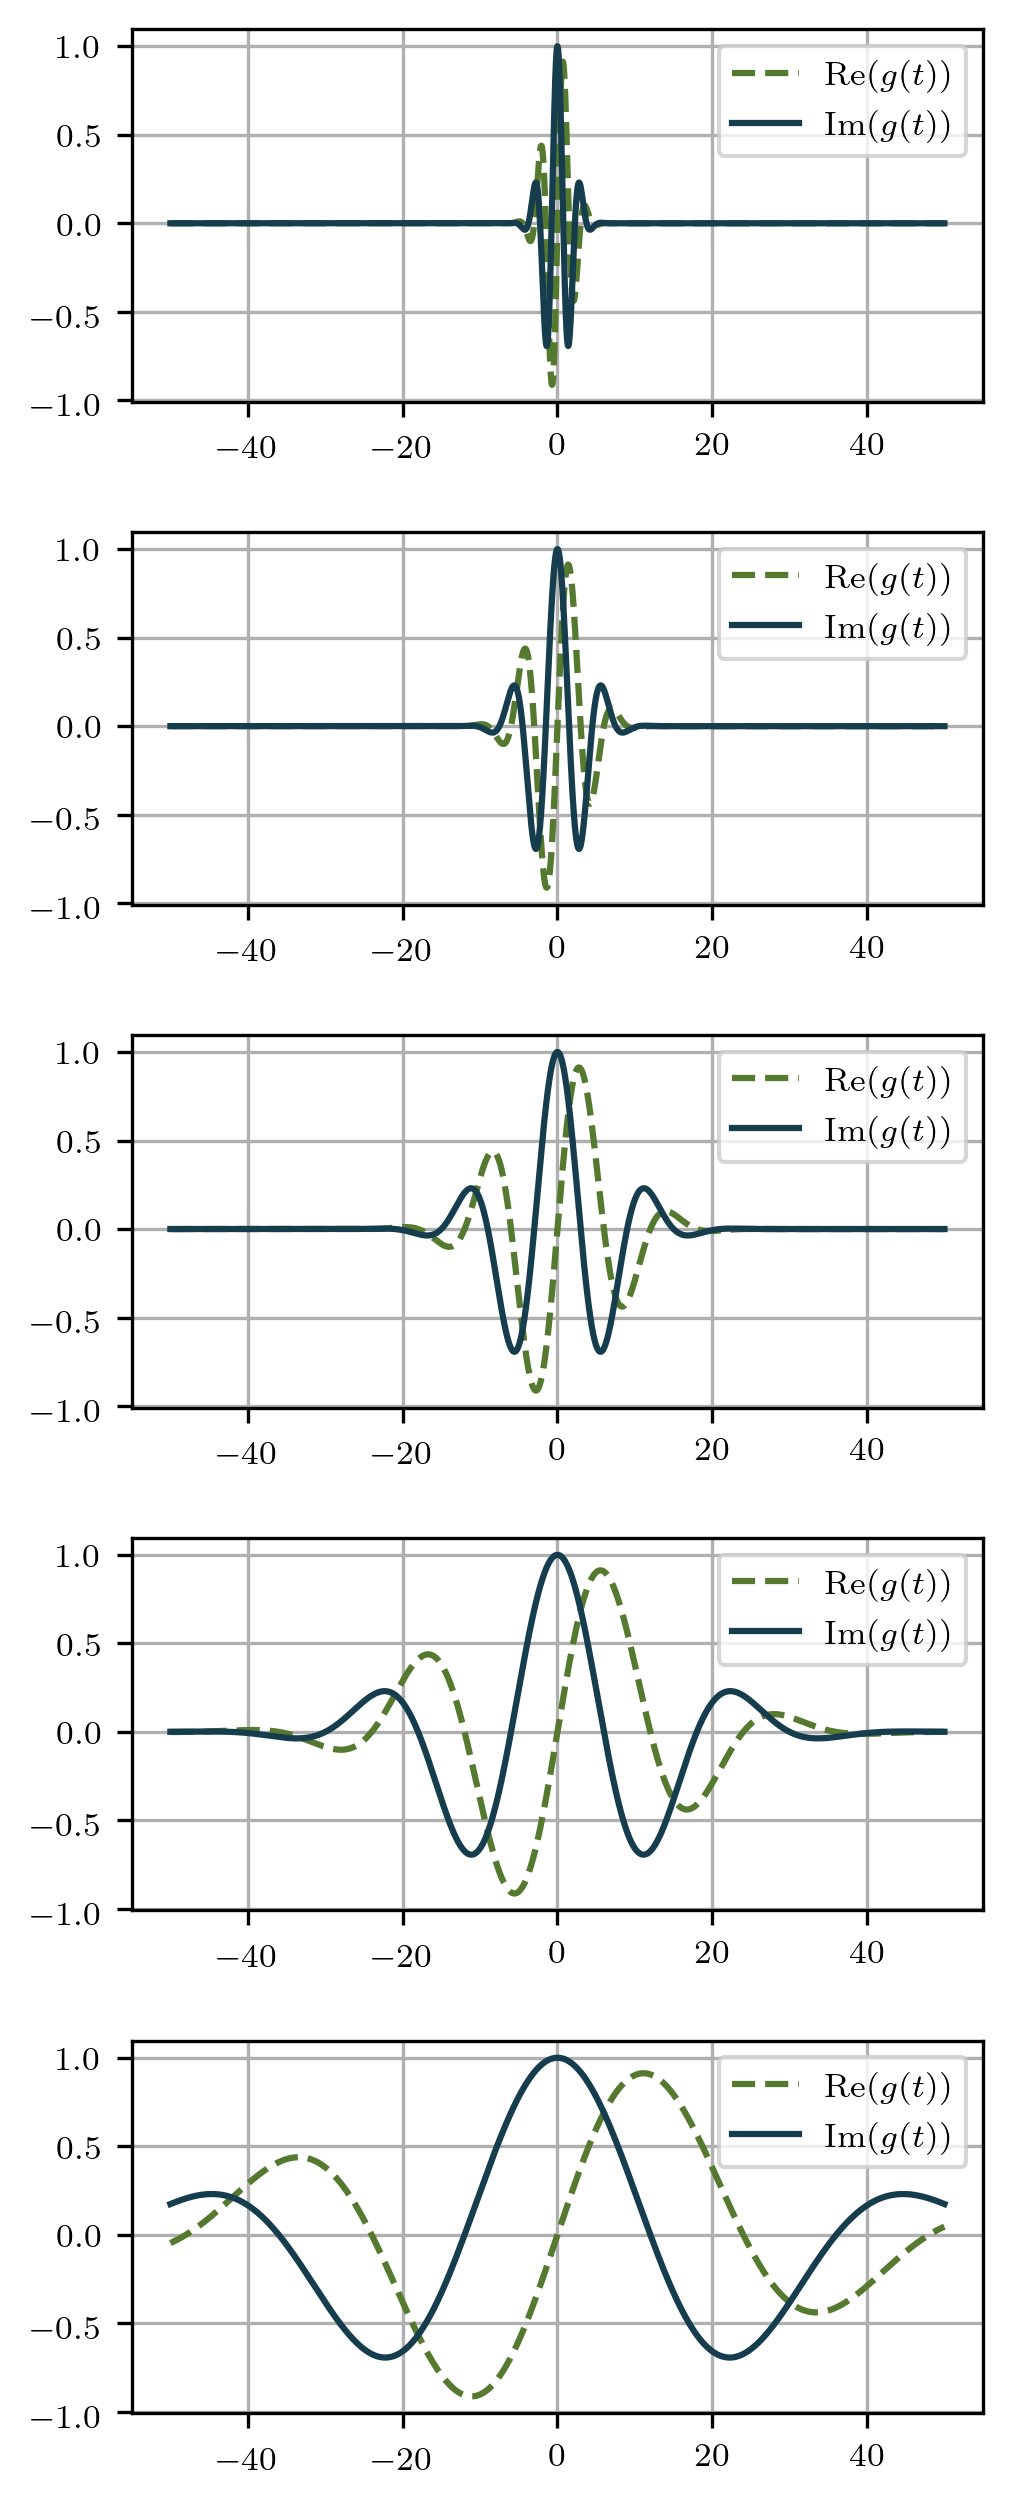
\includegraphics[width=\textwidth]{1D_space_GaborBank_m5_wo_env}
		\caption{$\kappa_{i} = \lbrace p: x \in [\pm 50] \rbrace$}
		\label{fig:1D_space_Gaborfilterbank_wo_env}
	\end{subfigure}
	\qquad %add desired spacing between images, e. g. ~, \quad, \qquad, \hfill etc. 
	%(or a blank line to force the subfigure onto a new line)
	\begin{subfigure}[b]{0.22\textwidth}
		\centering
		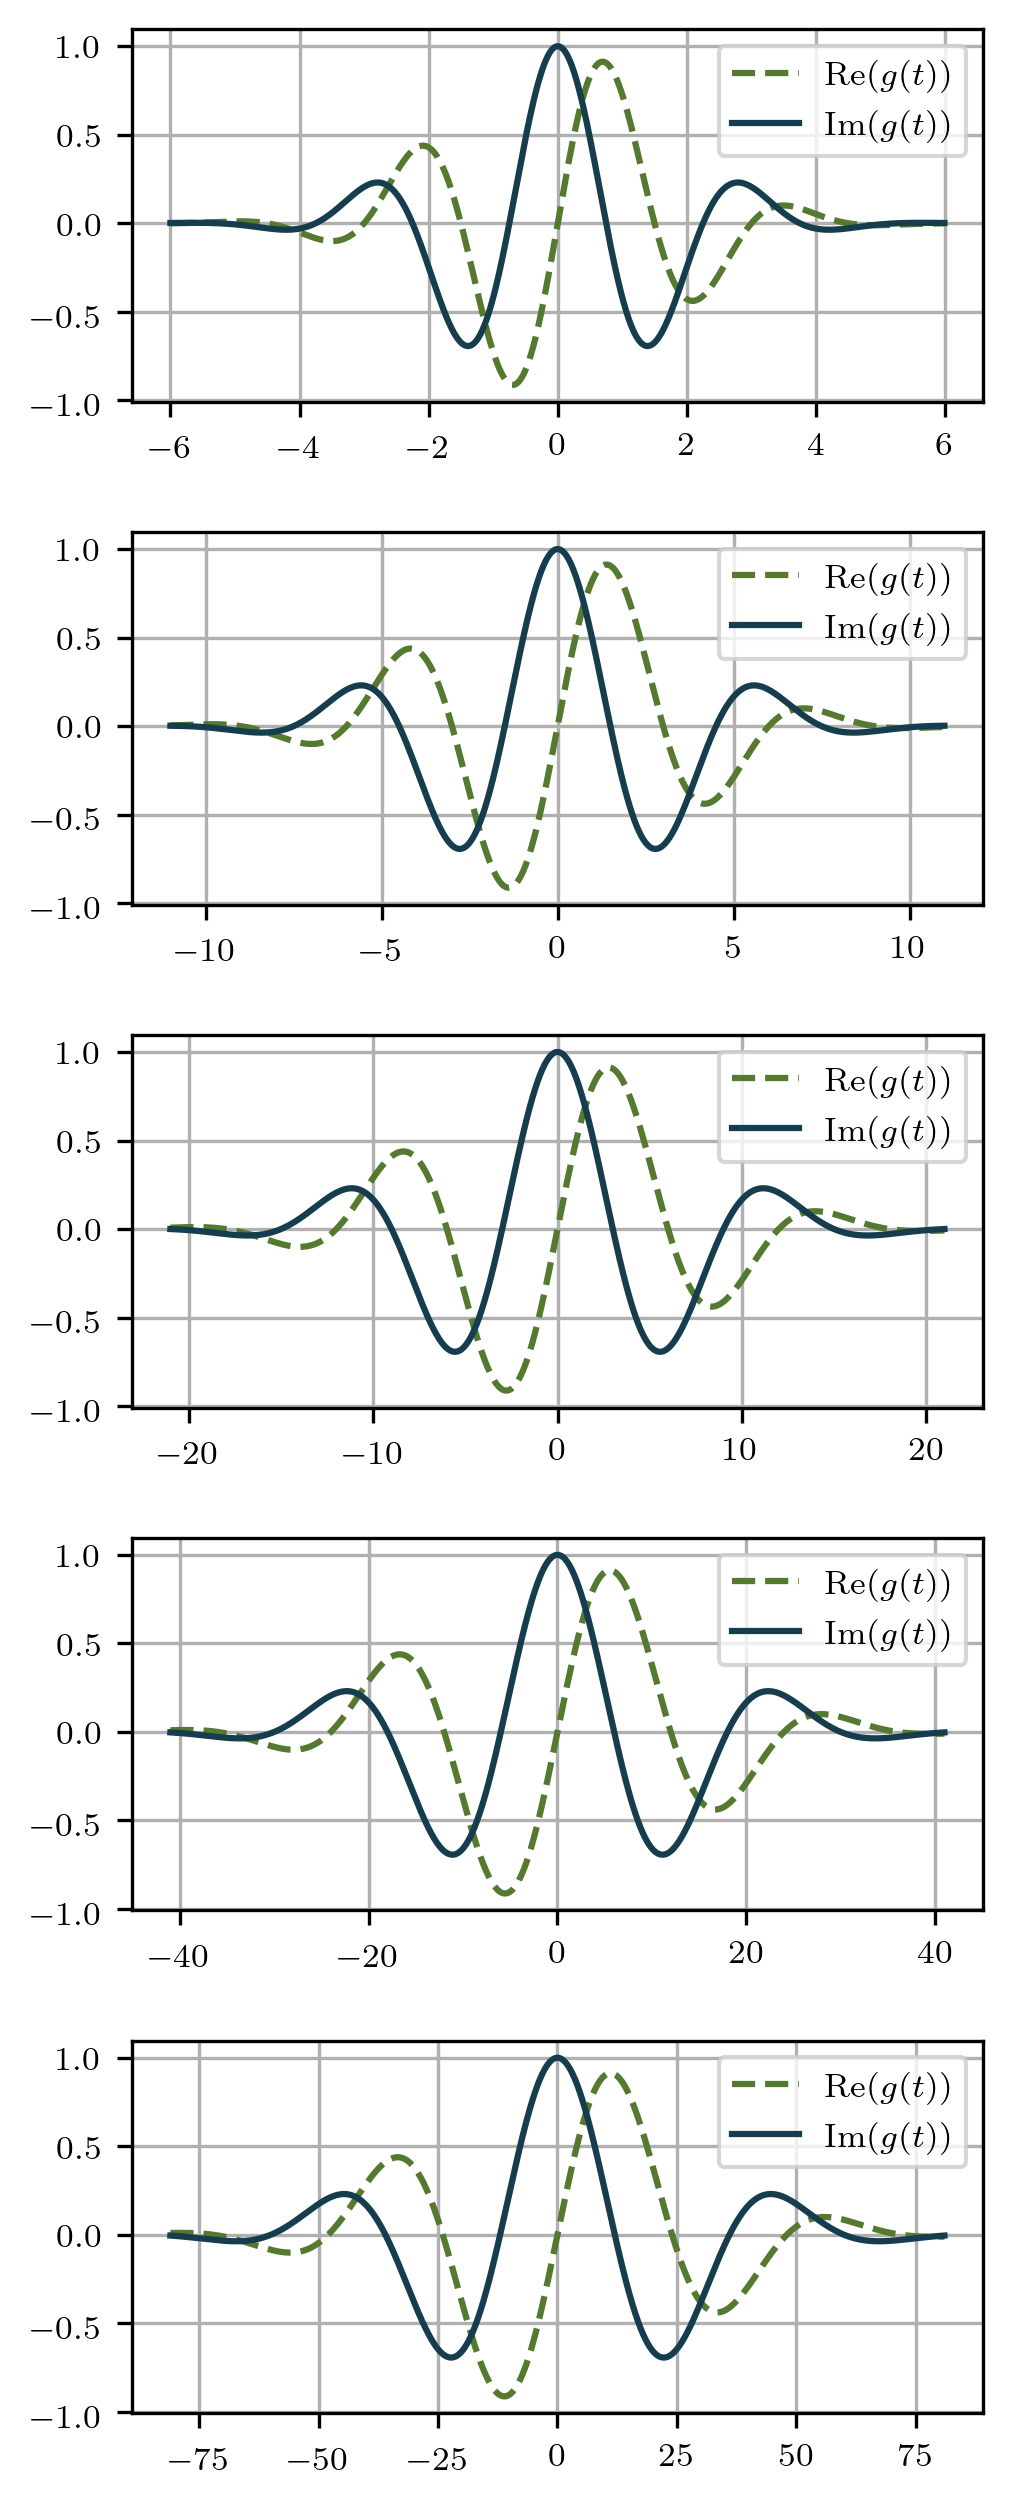
\includegraphics[width=\textwidth]{1D_space_GaborBank_m5_env}
		\caption{$\kappa_{i} = \lbrace p: x \in [\pm 3\sigma_{i}] \rbrace$}
		\label{fig:1D_space_Gaborfilterbank_env}
	\end{subfigure}

  \caption{Visual representation of the effective Gaussian envelope adaptation with filter bank with $M = 5$ frequencies in the space domain. \captext{(a)} Filter bank with no control over the envelope, \captext{(b)} Filter bank with control over the envelope's effective width.}
  \label{fig:1D_space_Gaborfilterbank}
\end{figure}


\subsubsection{Optimized 1-d Gabor function}
Gathering the different modifications of Gabor functions developed in the previous sections, we can define an optimized 1-d Gabor function as follows
\begin{equation}\label{eq:gabor_function_1d_timefreq_bank}
    \begin{gathered}
         g(t) =  \frac{f}{\gamma \sqrt{\pi}} e ^{-\left(\frac{f}{\gamma}\right)^2 t^2} e ^{j 2 \pi f t } \\
         G(\upsilon) =  e ^{-\left(\frac{\gamma \pi}{f}\right) ^2 (\upsilon-f)^2}
     \end{gathered}
\end{equation}

This Gabor function representation allows generating filter banks normalized by the maximum spectrum condition and homogeneously distributed in the frequency domain. Besides, a filter bank generated with the Gabor function Eq. \eqref{eq:gabor_function_1d_timefreq_bank} integrates the frequency crossing point allowing a quasi-total and almost flat coverage of the frequency spectrum, occupying the most relevant part of the filter using an adaptive window. A possible disadvantageous effect of this approach is the ripple between the filter bank's filters; however, we must remember that the filters proposed here are normalized concerning the size of the support (Gaussian window) and the central frequency of each filter. Therefore, even though a filter responds to different frequencies, textures close to the filter's center frequency are weighted. Additionally, the ripple effect occurs more frequently when decreasing the bandwidth of the filter bank. Moreover, this effect can be reduced by applying a halfwave rectification or, more generally called a thresholding \cite{Petkov:FGCS:1995}, \cite{Grigorescu.Petkov.ea:TIP:2003} \cite{Kruizinga.Petkov:TIP:1999}.

Figure \ref{fig:1d_filterbank_spacing} shows three examples of filter banks in the frequency domain.  Particulary, figure \ref{fig:filterbnk_octave_spacing} shows a bank without the relationship between the effective width and the central frequency of the filter, whereas the figures \ref{fig:filterbnk_half_crossingpoint} and \ref{fig:filterbnk_new_crossingpoint} show the interdependence between $\alpha$, $B_F$, $f$ and $c_1$ and the behavior of the bank with a different crossing point.

\subsection{2-d Gabor Filters}
The generalization of the Gabor function's theory from 1-d to 2-d is straightforward. First, we replace the time variable $t$ with the pair of spatial coordinates $(x, y)$ and the frequency variable $f$ with the pair of frequency variables $(u, v)$. Then, as for the 1-d case, the 2-d Gabor functions follows the Heisenberg principle where the uncertainty measures for the spatial and spatial-frequency domains are expressed in terms of $\Delta x$, $\Delta y$, $\Delta u$, and $\Delta v$, for which it holds that

\begin{equation}\label{eq:uncertainty_principle_2d}
    \begin{gathered}
        \Delta x\Delta u \geq \frac{1}{4\pi}\textrm{,} \quad \Delta y\Delta v \geq \frac{1}{4\pi}\textrm{and} \quad \Delta x \Delta y \Delta u \Delta v \geq \frac{1}{16\pi^2}
    \end{gathered}
\end{equation}

The 2-d Gabor function is represented by the modulated product of a harmonic oscillation with a pulse in the form of a probability function. The harmonic oscillation is represented by a complex exponential on any spatial frequency and any orientation; the pulse is represented by an elliptical Gaussian ellipse on any orientation. For simplicity, we assume that the orientation of the Gaussian and the harmonic modulation are the same and, therefore, define a compact form of the 2-d Gabor Elementary Function (GEF) in the space domain applying the given simplifications as follows
\begin{equation}\label{eq:gabor_function_2d_space_compact}
    \begin{gathered}
        g(x, r) =  e ^{-\left(\alpha^2 x_r^2 + \beta^2 y_r^2\right)} e ^{j 2 \pi f x_r } \\
        x_r = x \cos{\theta} + y \sin{\theta}\\
        y_r = -x \sin{\theta} + y \cos{\theta}
     \end{gathered}
\end{equation}

We obtain the analytical expression for the 2-d GEF in the spatial-frequency domain from the Fourier transform of Eq. \eqref{eq:gabor_function_2d_space_compact}, $G(u, v) = \mathcal{F}\{g(x, y)\}$, given by 
\begin{equation}\label{eq:gabor_function_2d_frequency_compact}
    \begin{gathered}
        G(u, v) =  \frac{\pi}{\alpha \beta} e ^{- \pi^2 \left(\frac{\left( u_r - f\right)^2}{\alpha^2} + \frac{v_r^2}{\beta^2}\right)} \\
        u_r = u \cos{\theta} + v \sin{\theta}\\
        v_r = -u \sin{\theta} + v \cos{\theta}
     \end{gathered}
\end{equation}

We can normalize the two above expressions following the same reasoning as in the 1-d case. We apply the maximum value condition \eqref{eq:maximun_condition} and the constant spectrum condition \eqref{eq:constant_spectrum_condition} described in section \ref{subsec:filter_normalization} to get $\max{|G(u,v)|} = 1$ and $\int_{-\infty}^{\infty} \int_{-\infty}^{\infty} |g(x,y)| dx dy = 1$ for a filter on any frequency $f$ and orientation $\theta$. 
Under these circumstances, the normalization constant is defined by
\begin{equation}\label{eq:normalization_constant_2d}
    \frac{\alpha \beta}{\pi}
\end{equation}
which applied to equations \eqref{eq:gabor_function_2d_space_compact}  and \eqref{eq:gabor_function_2d_frequency_compact}, gives us the normalized Gabor function in both 2-d domains. 

\begin{equation}\label{eq:gabor_function_2d_spacefrequency_normalized}
    \begin{gathered}
        g(x, r) = \frac{\alpha \beta}{\pi} e ^{-\left(\alpha^2 x_r^2 + \beta^2 y_r^2\right)} e ^{j 2 \pi f x_r } \\
        G(u, v) =   e ^{- \pi^2 \left(\frac{\left( u_r - f\right)^2}{\alpha^2} + \frac{v_r^2}{\beta^2}\right)} 
     \end{gathered}
\end{equation}

\subsubsection{Orientation filter spacing}

Equivalently than its 1-d version, the Gabor functions defined by equations \eqref{eq:gabor_function_2d_spacefrequency_normalized} do not cover most of the spectrum when we use them to build a filter bank at different frequencies and orientations (see Fig. \ref{fig:2d_filterbank_octave_spacing}); therefore, it does not help reconstruct a signal and the extraction of features. To obtain a more encompassing filter bank, it is evident that we need to include a relationship between the sharpness of the Gaussian window and the central frequency. 

The sharpness of the Gaussian function, unlike the 1-d case, now includes two variables ($\alpha, \beta$) that affect the effective width of the Gabor filter envelope. Such an envelope can have an elliptical shape, where $\alpha $ controls the length of the major axis and $\beta$ controls the length of the minor axis. 

The analysis of the frequency separation between adjacent filters of a bank viewed in the section \ref{subsec:frequency_filter_spacing} is also valid in the 2-d case. Thus, the full bandwidth of half the frequency response, $B_F$, represents the separation between the center frequencies; the interval $\Delta f$ represents the distance between the points where $G(u, v)$ begins to decrease and; the full frequency bandwidth through the ratio $\gamma$ and the crossing point $c_1$ allows adapting the size of the major axis of the envelope $\alpha$ depending on the center frequency $f$.

We can do a similar analysis for the minor axis of Gabor's envelope. First, notice that insertion of the orientation variable $\theta$ in the 2-d case implies the existence of an angular separation $B_{\theta}$ between the centers of the filters in a bank (see Fig. \ref{fig:2d_filterbank_octave_spacing}). This angular bandwidth can be defined by the total number of orientations $N$ in a filter bank such that
\begin{equation}\label{eq:angular_bandwidth}
    B_{\theta} = \frac{\pi}{N}
\end{equation}
and threfore, we can obtain the the filter bank's orientation angles as 
\begin{equation}\label{eq:filterbank_angles}
    \theta_n = n \frac{\pi}{N} \textrm{,} \quad n = \{0, \cdots, N-1\}
\end{equation}

We propose to vary the length of $\beta$ as a function of the central frequency and the angular bandwidth through an angular interval $\Delta \theta$, which is the distance along $\beta$ where $G(u, v)$ begins to decrease.

\begin{equation}\label{eq:orientation_interval_crossing_point}
    \frac{\Delta \theta}{2} = \frac{\beta}{\pi}\sqrt{\ln \left(\frac{1}{c_2}\right)}
\end{equation}

\begin{figure}[!ht]
\centering
    \subcaptionbox{\label{fig:2d_filterbank_octave_spacing}}{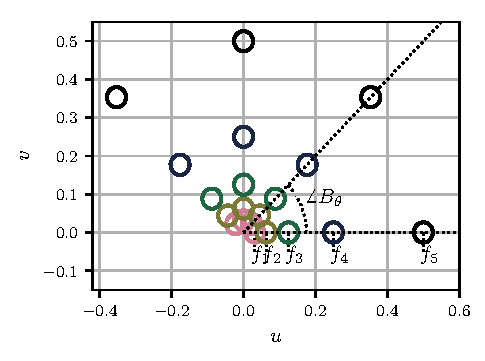
\includegraphics[width=0.24\textwidth]{GaborFilterbank_freq_2d_octave_spacing.pdf}}
    \subcaptionbox{\label{fig:2d_filterbank_half_crossingpoint}}{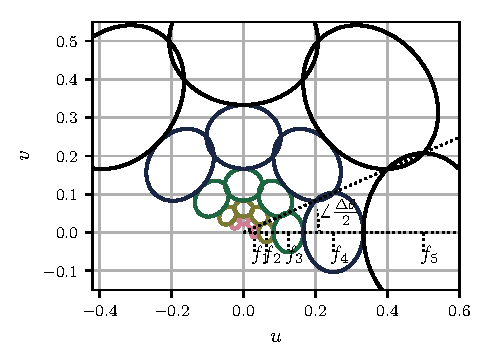
\includegraphics[width=0.24\textwidth]{GaborFilterbank_freq_2d_half_crossingpoint.pdf}}    
\caption{Filter spacing and crossing point effect represented on a 2-d filter bank in the frequency domain: \captext{(a)} Filters separation without crossing points between adjacent filters $[B_F=1, B_{\theta} = 45^{\circ}, \alpha=\beta=0.1, c_1=c_2=-]$, \captext{(b)} Filters separation with crossing points between adjacent filters $[B_F=1, B_{\theta} = 45^{\circ}, \alpha=f/\gamma, \beta=f/\eta, c_1=c_2=0.9]$. High and low cut-off frequency points given by $\Delta f$ and $\Delta \theta$.}\label{fig:2d_filterbank_spacing}
\end{figure}

We know that for a filter whose center frequency is $f$ and whose cut-off angular interval is $\Delta \theta$, the full orientation bandwidth $B_\theta$ expressed in radians is defined as \cite{Daugman:JOSA:1985}.
\begin{equation}\label{eq:orientation_bandwidth_interval}
    B_{\theta} = 2 \tan^{-1} \left( \frac{\Delta \theta}{2f} \right)
\end{equation}

It is clear that using expression \eqref{eq:orientation_interval_crossing_point} in equation \eqref{eq:orientation_bandwidth_interval}, we find the expression that relates the frequency bandwidth to the central frequency and the length of the Gaussian minor axis.
\begin{equation}\label{eq:orientation_bandwidth}
    B_{\theta} = 2 \tan^{-1} \left( \frac{\beta}{\pi f} \sqrt{\ln \left(\frac{1}{c_2}\right)} \right)
\end{equation}

Taking the above relationships permits to write the 2-d GEF to use it into a bank as follows. 

\begin{equation}\label{eq:gabor_function_2d_spacefreq_bank}
    \begin{gathered}
         g(x,y) =  \frac{f^2}{\gamma \eta \pi} e ^{-\left(\frac{f^2}{\gamma^2} x_r^2 + \frac{f^2}{\eta^2} y_r^2\right)} e ^{j 2 \pi f x_r } \\
         G(u,v) =  e ^{-\left(\frac{\pi}{f}\right)^2\left( \gamma^2 (u_r-f)^2 + \eta^2 v_r^2\right)}
     \end{gathered}
\end{equation}
where now the length $\alpha$ of each filter in the bank will be determined based on the ratio $\gamma = \frac{f}{\alpha}$ and crossing point between adjacent filters $c_1$; and the length $\beta$ will be determined based on the ratio $\eta = \frac{f}{\beta}$ and crossing point between adjacent filters $c_2$.

Figure \ref{fig:2d_filterbank_spacing} shows the octave spacing and the orientation bandwidth for a bank of filters in the frequency domain. Particulary, figure \ref{fig:2d_filterbank_octave_spacing} shows a bank without the relationship between the effective width and the central frequency of the filter, whereas figure \ref{fig:2d_filterbank_half_crossingpoint} show the interdependence between $\alpha$, $\beta$, $B_F$, $B_{\theta}$, $f$ and the crossing points $c_1$, $c_2$.

\begin{figure}[!ht]
	\centering
	\begin{subfigure}[b]{0.4\textwidth}
		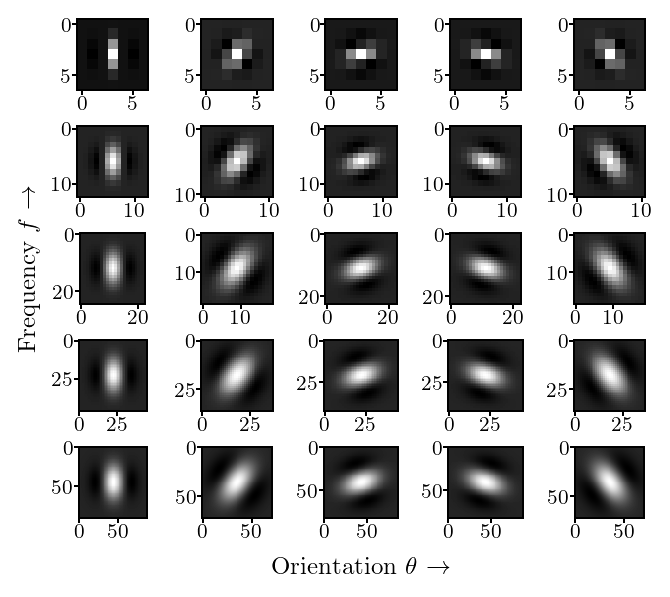
\includegraphics[width=\textwidth]{GaborFilterbank_spatial_2d_real}
		\caption{Real part}
		\label{fig:2d_filterbank_real}
	\end{subfigure}\\
	\begin{subfigure}[b]{0.4\textwidth}
		\centering
		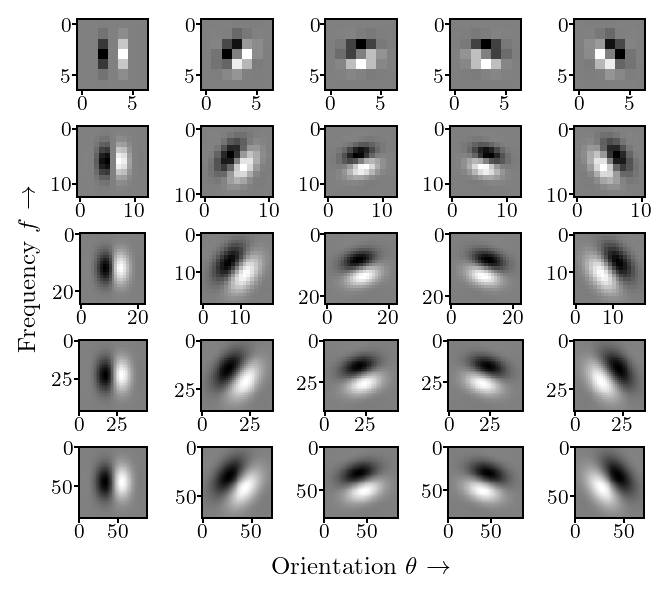
\includegraphics[width=\textwidth]{GaborFilterbank_spatial_2d_imag}
		\caption{Imaginary part}
		\label{fig:2d_filterbank_imag}
	\end{subfigure}
	    
    \caption{Custom designed Gabor filter bank. The design parameters are: max/min period $[1/f_{min}=70, 1/f_{max}=4]$, crossing points (frequency and angular) $[c_1=c_2= 0.9]$, bandwidths (frequency and angular) $[B_F=1, B_{\theta} = 35^{\circ}]$, standard devaitions $[\sigma=3]$.}\label{fig:2d_filterbank}
\end{figure}


\section{Complex Color Space}
Color spaces mostly map the perception of color as a three-dimensional property. However, these dimensions can be encompassed in only two aspects; therefore, we can classify them into luminance-chromaticity and luminance-chrominance color spaces. In both cases, luminance is the property that describes the brightness of the light; however, both categories have different ways of defining color. Chromaticity-based spaces define color independently of luminance (or the luminance equivalent in a particular color space). In a chrominance-based space, the chrominance values of the image change as the light intensity varies.
  
We can obtain a color space based on chromaticity from the classic trichromatic models described in the previous section. The chromaticity of these models consists mainly of two independent parameters. For example, the $xyY$ color space, from which we obtain the CIE chromaticity chart (see figure \ref{fig:chrom_diagram}), uses the X and Y dimensions to calculate chromaticity. In RGB space, it is possible to obtain a space based on chromaticity following the same principle, using only the R and G channels for its calculation. For cylindrical color spaces (HSV, HSL), the independent parameters that describe the chromaticity are hue and colorfulness (saturation) dimensions.

\begin{figure}[!ht] 
	\centering
	\begin{subfigure}[b]{0.22\textwidth}
		\centering
		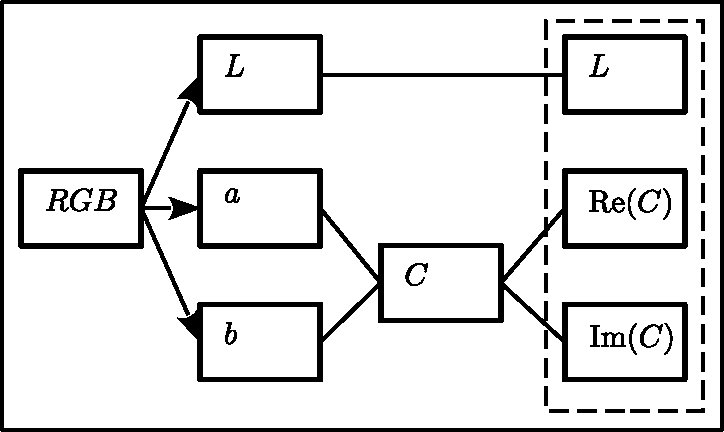
\includegraphics[width=\textwidth]{lab_complex_color}
		\caption{}	
		\label{fig:lab_complex_color}
	\end{subfigure}
	~%add desired spacing between images, e. g. ~, \quad, \qquad, \hfill etc. 
	%(or a blank line to force the subfigure onto a new line)
	\begin{subfigure}[b]{0.22\textwidth}
		\centering
		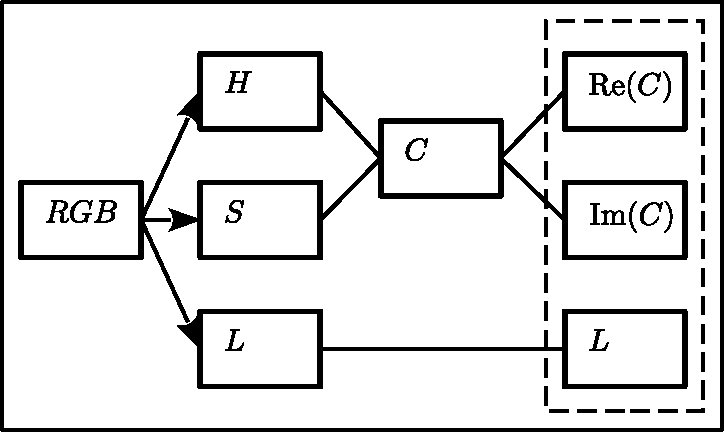
\includegraphics[width=\textwidth]{hsl_complex_color}
		\caption{}	
		\label{fig:hsl_complex_color}
	\end{subfigure}
	~%add desired spacing between images, e. g. ~, \quad, \qquad, \hfill etc. 
	%(or a blank line to force the subfigure onto a new line)
	\begin{subfigure}[b]{0.22\textwidth}
		\centering
		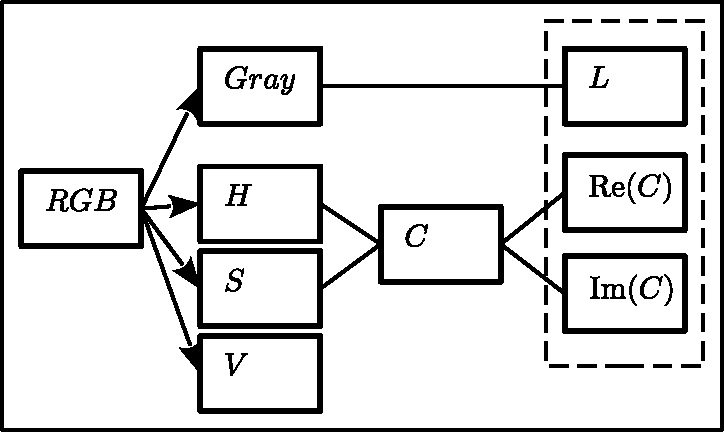
\includegraphics[width=\textwidth]{hsv_complex_color}
		\caption{ }	
		\label{fig:hsv_complex_color}
	\end{subfigure}
	
	\caption{Graphic display of tree alternatives to obtain the complex color representation of an image: \captext{(a)} form LAB color space, \captext{(b)} from form HSL color space, and \captext{(c)} from HSV color space.}
	\label{fig:complex_color_spaces}
\end{figure}

The chromaticity-based models are reputed for their use in image editing and color correction. However, the chrominance-based spaces are helpful if we are looking for a uniform distribution of the color information in an image. Some examples of color spaces in this category are CIELAB and CIELUV. In them, the colorfulness information of an image is found in channels A and B (resp. U and V), and the final color is defined by the brightness of the light defined by the luminance L.

The use of spaces based on luminance-chrominance reduces the dimensionality of the color to two channels $L$ and $C$.To make this two-channel color representation possible, we combine the values of channels A and B with the chrominance function.
\begin{equation}\label{eq:chrominance_lab}
    C = A + \mathsf{i}B
\end{equation}

In the same way, it is possible to obtain a luminance-chrominance color space using the dimensions of the cylindrical HSV/HSL color spaces. In that case, the hue H and saturation S channels describe the chrominance such that the function
\begin{equation}\label{eq:chrominance_hsv}
    C = S \mathsf{e}^{\mathsf{i}H}
\end{equation}
defines the complex chrominance channel.

These representations have the advantage of reducing the dimensionality of the color information. In image processing, we can obtain these color spaces from the transformation of the image from the RGB space to the LAB, HSV, and HSL spaces, from which we get the chrominance variables and, consequently, the complex chrominance channel. Regarding the luminance, it may differ depending on the input color space. For example, for the LAB and HSL spaces, this variable is naturally defined; however, in the HSV space, the luminance channel is obtained from transforming the RGB input image to a grayscale image. Figure \ref{fig:complex_color_spaces} shows the diagrams for obtaining an image represented in two channels.

%\begin{figure}[!ht]
%    \begin{subfigure}[t]{\dimexpr0.3\textwidth+20pt\relax}
%    	\makebox[20pt]{\raisebox{35pt}{ \rotatebox[origin=c]{90}{\captext{Input image}} }}%
%    	\includegraphics[width=\dimexpr\linewidth-20pt\relax]{araras}
%    \end{subfigure} \\    
%     
%    \begin{subfigure}[t]{\dimexpr0.3\textwidth+20pt\relax}
%    	\makebox[20pt]{\raisebox{35pt} {\rotatebox[origin=c]{90}{\captext{HSV luma/chroma}} }}%
%    	\includegraphics[width=\dimexpr\linewidth-20pt\relax]{araras_lum_HSV}
%    \end{subfigure}      
%    ~ %add desired spacing between images, e. g. ~, \quad, \qquad, \hfill etc. 
%      %(or a blank line to force the subfigure onto a new line)
%    \begin{subfigure}[b]{0.3\textwidth}
%        \includegraphics[width=\textwidth]{araras_chrr_HSV}
%    \end{subfigure}
%    ~ %add desired spacing between images, e. g. ~, \quad, \qquad, \hfill etc. 
%      %(or a blank line to force the subfigure onto a new line)
%    \begin{subfigure}[b]{0.3\textwidth}
%        \includegraphics[width=\textwidth]{araras_chri_HSV}
%    \end{subfigure} \vspace{5pt}      
%    
%    \begin{subfigure}[t]{\dimexpr0.3\textwidth+20pt\relax}
%    	\makebox[20pt]{\raisebox{35pt} {\rotatebox[origin=c]{90}{\captext{HSL luma/chroma}} }}%
%    	\includegraphics[width=\dimexpr\linewidth-20pt\relax]{araras_lum_HLS}
%    \end{subfigure}     
%    ~ %add desired spacing between images, e. g. ~, \quad, \qquad, \hfill etc. 
%      %(or a blank line to force the subfigure onto a new line)
%    \begin{subfigure}[b]{0.3\textwidth}
%        \includegraphics[width=\textwidth]{araras_chrr_HLS}
%    \end{subfigure}
%    ~ %add desired spacing between images, e. g. ~, \quad, \qquad, \hfill etc. 
%      %(or a blank line to force the subfigure onto a new line)
%    \begin{subfigure}[b]{0.3\textwidth}
%        \includegraphics[width=\textwidth]{araras_chri_HLS}
%    \end{subfigure} \vspace{5pt} 
%    
%    \begin{subfigure}[t]{\dimexpr0.3\textwidth+20pt\relax}
%    	\makebox[20pt]{\raisebox{35pt} {\rotatebox[origin=c]{90}{\captext{LAB luma/chroma}} }}%
%    	\includegraphics[width=\dimexpr\linewidth-20pt\relax]{araras_lum_LAB}
%    \end{subfigure}     
%    ~ %add desired spacing between images, e. g. ~, \quad, \qquad, \hfill etc. 
%      %(or a blank line to force the subfigure onto a new line)
%    \begin{subfigure}[b]{0.3\textwidth}
%        \includegraphics[width=\textwidth]{araras_chrr_LAB}
%    \end{subfigure}
%    ~ %add desired spacing between images, e. g. ~, \quad, \qquad, \hfill etc. 
%      %(or a blank line to force the subfigure onto a new line)
%    \begin{subfigure}[b]{0.3\textwidth}
%        \includegraphics[width=\textwidth]{araras_chri_LAB}
%    \end{subfigure} \vspace{5pt} 
%        
%    \caption{Color channels of an image in different color spaces in grayscale.}\label{fig:images_color_complex_space}    
%\end{figure}

%Figure \ref{fig:images_color_complex_space} shows the transformation of a natural image (first row of the figure array) from RGB space to complex two-channel color space. Each row in the figure shows the luminance channel and the two parts (real and imaginary) of the chrominance channel. Note that as it happened in the representation of the classic color spaces (figure \ref{fig:images_color_space}) since the method to compute saturation differs in HSV and HSL spaces, the chrominance channel is different. The same effect occurs with the L luminance channel from LAB space and the luminance from the RGB to gray transformation; in theory, both are the same, but we can see differences in practice.

\section{The Gabor-filter-based Complex Color Feature Space}
\subsection{Color Image Transformation}
The first stage in creating the feature space is transforming the input image from the RGB color space to the two-channel luminance-chrominance space. The representation in two channels, one real and the other complex, of a color image allows us to separate the intervention of luminance and colors in the generation of textures in an image. To help visualize such a joint phenomenon, we create a synthetic image that reflects the complexity of natural color images.

\subsubsection{Synthetic image description}
The synthetic image we create contains seven different regions with spatial variations (textures) generated by alternating various colors at different frequencies. Each tile of the image is perceived as a whole; this is perceptually a constant region. The colors alternate along different directions in the chrominance phase (Fig. \ref{fig:color_complex_plane}). The last image region has two frequency components.

We generate the input image with the sign function of a 2-d sinusoidal signal multiplied by the color values of each region in the RGB color space such that
\begin{gather}
	I(x, y) = sgn( \sin 2 \pi (f_x x_r + f_y y_r)) \cdot [R, G, B]\label{eq:2D_squared_signal}\\
	x_r = x \cos\theta + y \sin\theta \nonumber \\
    y_r = -x \sin\theta + y \cos\theta \nonumber  
\end{gather}

We control the image texture by varying the frequencies $f_{x}, f_{y}$ and the orientation angle $\theta$ of the coordinate plane $(x, y)$, where $\theta=0^\circ$ means vertical variations and $\theta=90^\circ$ horizontal variations. The proposed image has a size of $320\times1400$ pixels. The seven characteristic regions of the image are spread over $1400$ pixels wide, so each region is about $320\times200$ pixels; that is, the color/texture distribution in the image changes every 200 pixels (on the $x$-axis). The following expressions define the spatial image variations.  
\begin{gather}
	f_{x} = 
	\begin{cases} 
      0    & 0\leq x\leq 200  \\
      1/64 & 201\leq x\leq 400  \\
      1/32 & 401\leq x\leq 600  \\
      1/16 & 601\leq x\leq 800  \\
      1/8  & 801\leq x\leq 1000  \\
      1/4  & 1001\leq x\leq 1200 \\   
      1/8  & 1201\leq x\leq 1400 \\ 
   	 \end{cases} \nonumber ; \quad
   	 f_{y} = \begin{cases} 
      0    & 0\leq x\leq 200  \\
      0    & 201\leq x\leq 400  \\
      0    & 401\leq x\leq 600  \\
      0    & 601\leq x\leq 800  \\
      0    & 801\leq x\leq 1000  \\
      0    & 1001\leq x\leq 1200 \\  
      1/32 & 1201\leq x\leq 1400 \\ 
   	 \end{cases} \nonumber  
\end{gather}

For comprehension purposes, we use colors easily identified in the RGB space (primary colors) or in the HSV space (perceptual colors) to generate the image textures. Figure \ref{fig:synthetic_color_texture_image} depicts the resulting synthetic image. 

\begin{figure}[!ht]
    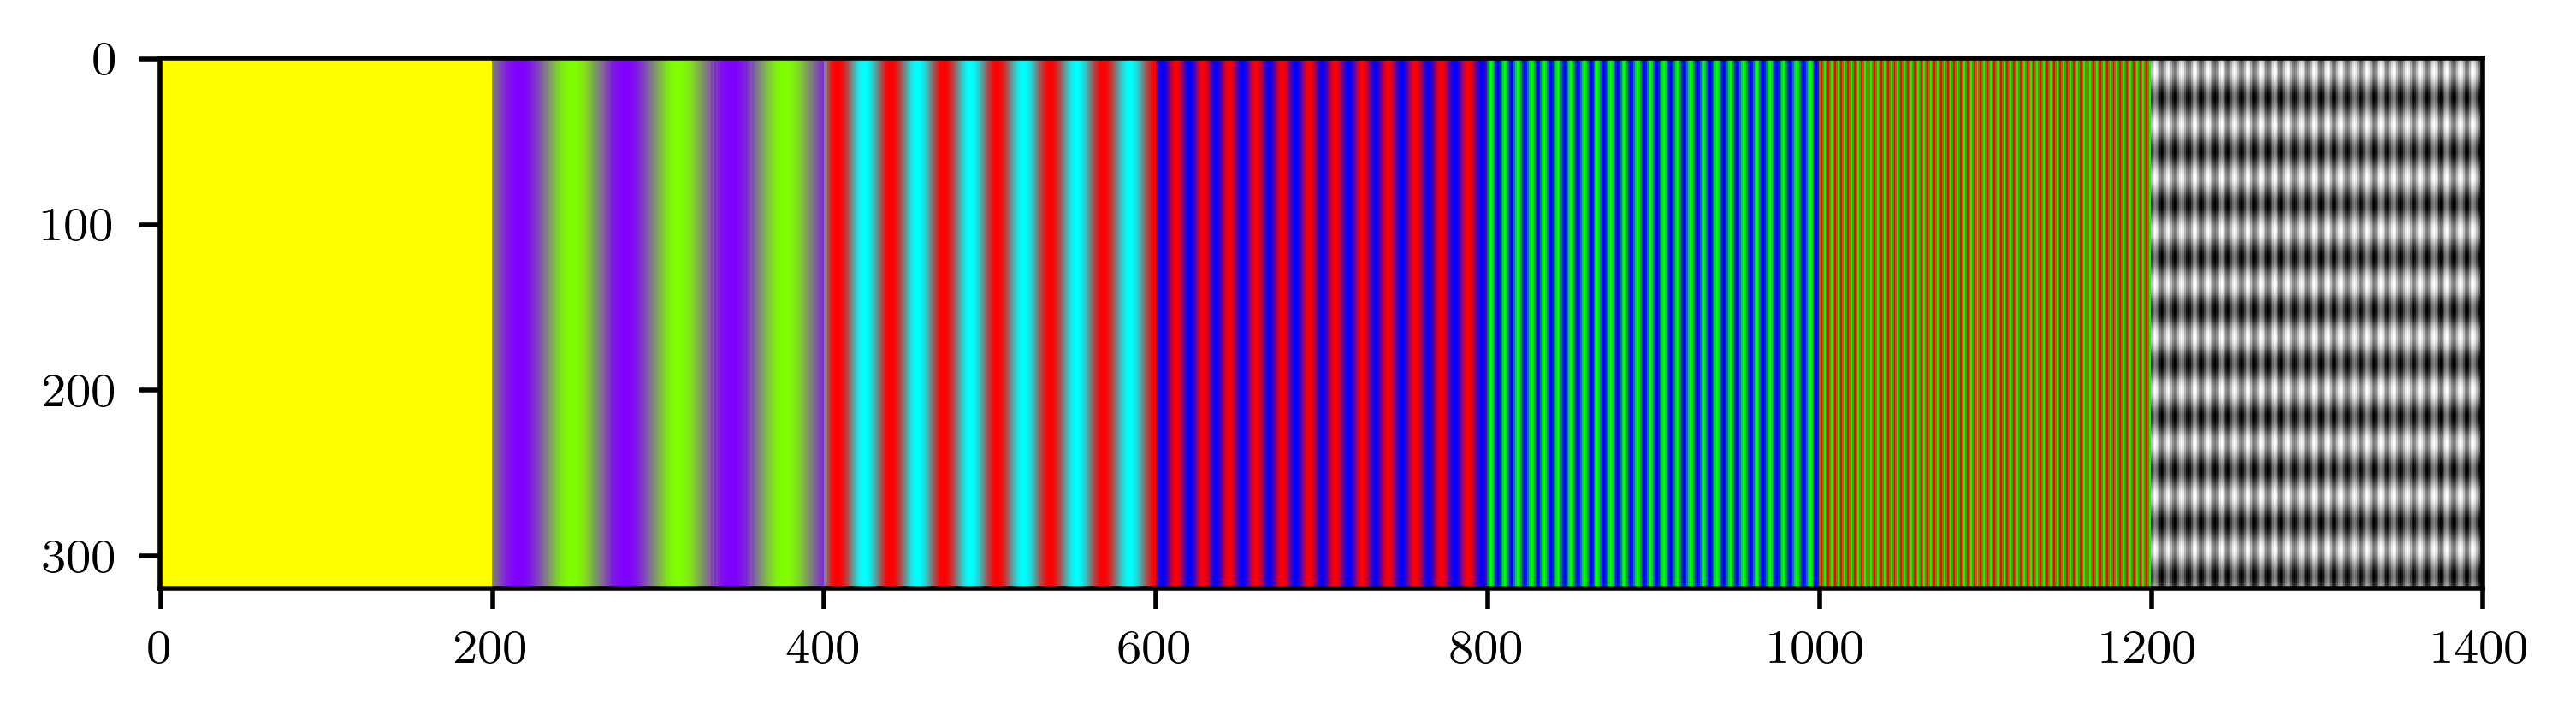
\includegraphics[width=0.5\textwidth]{synthetic_image_color_texture}
\caption{Synthetic color textured image.}\label{fig:synthetic_color_texture_image}
\end{figure}

The 2-d sinusoidal modulations generate textures in the image at different and well-known frequencies. These modulations change the colors of the regions generating a texture of oriented lines. The regions of the synthetic image have the following color and texture characteristics.

\paragraph{Region 1. Textureless zone:}
This region does not contain spatial variations, i.e., it has only a solid color. The color of the region is yellow (arbitrarily chosen).

\paragraph{Region 2. Lowest frequency textured zone with colors on the imaginary plane:}
This region is described by the vertical texture generated by variations between purple and green lime. Such colors are found in the imaginary axis of the chrominance plane. The colors in this region change every 64 pixels (along the $x$-axis).

\paragraph{Region 3. Textured zone with colors on the real plane:}
This region contains a vertical texture generated by the variations between red and cyan. Such colors are found in the real axis of the chrominance plane. The colors in this region change every 32 pixels (along the $x$-axis).

\paragraph{Region 4. Textured zone with two primary colors:}
The variations between red and blue generate the horizontal texture of this region. The colors in this region change every 16 pixels (along the $x$-axis). 

\paragraph{Region 5. Textured zone with two primary colors:}
The variations between blue and green generate the horizontal texture of this region. The colors in this region change every 8 pixels (along the $x$-axis). 

\paragraph{Region 6. Textured zone with two primary colors:}
The variations between green and red generate the horizontal texture of this region. The colors change every 4 pixels (along the $x$-axis).

\paragraph{Region 7. Colorless mixed textures zone:}
This region contains two textures, both of them formed by the variations between black and white, i.e., there is no color information. Moreover, the textures change in frequency and orientation; the pixes of the horizontal texture change of color every 4 pixels along the $x$-axis (highest frequency), while the pixel values of the vertical texture changes every 16 pixels along the $y$-axis (same frequency as region 4).

We summarize the colors and frequency of each zone in Table \ref{tab:synthetic_image_components}. In the table, we expose the $RGB$ and $HSV$ values of the texture-forming colors as well as the frequency and orientation of each section.

\subsubsection{Graphical Display of the Synthetic Image Color Distribution}
The choice of texture-forming colors comes from the interest in visualizing the color spectrum of the image more graphically. The two-channel color spaces, described in chapter \ref{ch:color_texure_representations}, encode color information in a complex chrominance channel. Therefore, we can interpret the chrominance values as points within a complex plane (see Fig. \ref{fig:color_complex_plane}). In the case of LAB/LUV spaces, the values of chrominance are defined in Cartesian coordinates as 
\begin{equation}\label{eq:chrominance_lab2}
    C = A + \mathsf{i}B
\end{equation}
where channel A values represent the real axis coordinates, and channel B values represent the imaginary axis coordinates. 

HSV/HSL color spaces encode chrominance values as points in polar coordinates 
\begin{equation}\label{eq:chrominance_hsv2}
    C = S \mathsf{e}^{\mathsf{i}H}
\end{equation}
where channel H values are the angle expressed radians and channel S values are the distance from the origin to the color points.

Considering these two chrominance configurations, the one defined by hue and saturation provides a more straightforward geometric interpretation of chrominance. Originally hue is a cylindrical dimension representing the color tints in the chromatic circle as angles, while saturation, which represents the purity of color, places achromatic tints in the center of the circle and pure colors on the circular edge of the disk. In figure \ref{fig:color_complex_plane}, we show the synthetic image color distribution plot using the HS dimensions in the 2-d chrominance complex plane. The hue $H$ is expressed in degrees, and saturation $S$ is normalized between $0$ and $255$. This representation complements the description of our synthetic test image Fig. \ref{fig:synthetic_color_texture_image}, showing the variation between colors that generate textures. We can notice in the chroma circle of figure \ref{fig:color_complex_plane} the transition between the red-green-blue primary colors at $0^\circ$, $120^\circ$ and $240^\circ$ respectively; the transition between purple and lime green on the imaginary axis with a hue of $90^\circ$ and $270^\circ$ respectively; the transition between red at $0^\circ$ and cyan at $180^\circ$ passing through the real axis of the plane and finally; the yellow color with a hue value of $60^\circ$.

\begin{figure}[!ht]
	\centering
    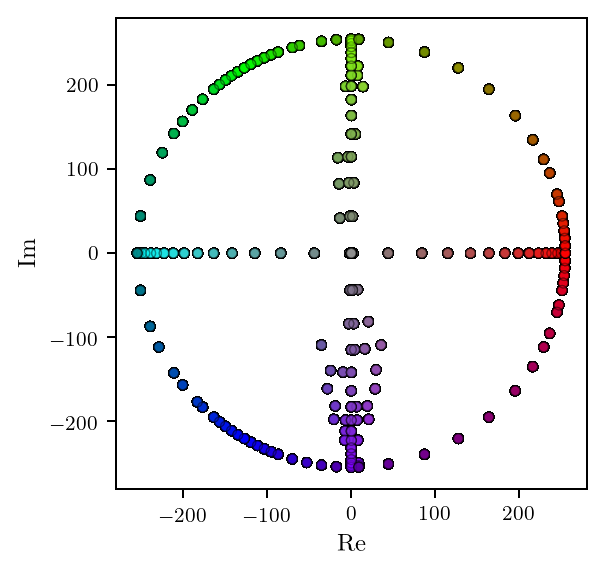
\includegraphics[width=0.4\textwidth]{color_complex_plane}
	\caption{Synthetic image chrominance distribution represented in the color complex plane.}\label{fig:color_complex_plane}
\end{figure}

Under this color space configuration, the colors of an image are represented in the complex chrominance plane. However, in this plane, the variations due to luminance information do not appear. The brightness of the colors is captured in the luminance channel. Depending on the color space that we use to build the two-channel color representation, we can obtain the luminance channel differently. In the LAB/LUV and HSL color spaces, the luminance channel is directly represented by the $L$ dimension values. In the HSV color space, we use the image transformation from RGB to gray-scale following the Eq. \eqref{eq:color2gray_formula} to obtain the luminance channel.

Figure \ref{fig:three_channel_decomposition} shows the three dimensions of the two-channel representation of the synthetic image ($L(x,y)$, $\RE(C(x,y))$, $\IM(C(x,y))$) in grayscale. In this representation, we use the HSV color space as a basis to obtain the luminance and chrominance values, so the $L$ channel is obtained with Eq. \eqref{eq:color2gray_formula} and the $C$ channel with Eq. \eqref{eq:chrominance_hsv2}. In figure \ref{fig:three_channel_decomposition}, we can see how the different regions show more or less important values depending on the channel in which they are. For example, the horizontal and vertical spatial variations of region 7 (between 1200 and 1400 column pixels) are only visible in the luminance channel $L(x,y)$ (see left image in \ref{fig:three_channel_decomposition}). We observe this same effect in the chrominance channels, for example, with the vertical textures of region 3. The spatial variations of this region are made up by the alternation of colors that live only in the real plane of chrominance (red and cyan), so the texture is only visible in channel $\RE(C(x,y))$ (see column pixels between 400 and 600 of the central image and the image to the right of subfigure \ref{fig:three_channel_decomposition}). 

We can also visualize the color variations and their influence on the generation of textures by plotting a horizontal line using a row of pixels' intensity values for each dimension of the two-channel space. In figure \ref{fig:horizontal_line_three_channel_decomposition}, we show the variations generated by changes in color and (or) lightness in a 1-d plot. Taking the area without texture (region 1), the horizontal line between pixels 0 and 200 remains constant in all three channels due to the absence of texture. However, in region 2, which corresponds to the low-frequency texture formed by the colors at $90^\circ$ and $270^\circ$ in the chroma circle, we see that variations are only present in the imaginary channel of chrominance $\IM(C(x,y))$. In regions 4, 5, and 6, since the texture-forming colors are two of the three primary colors (red, green, blue), the variations are visible in all three luminance-chrominance representation channels. Finally, in the last region (colorless mixed textures zone), we can see that the variations are only present in the channel that describes the luminance $L(x,y)$.

\begin{figure}[!ht]
\centering
    \subcaptionbox{\label{fig:synthetic_image_three_channel_decomposition}}{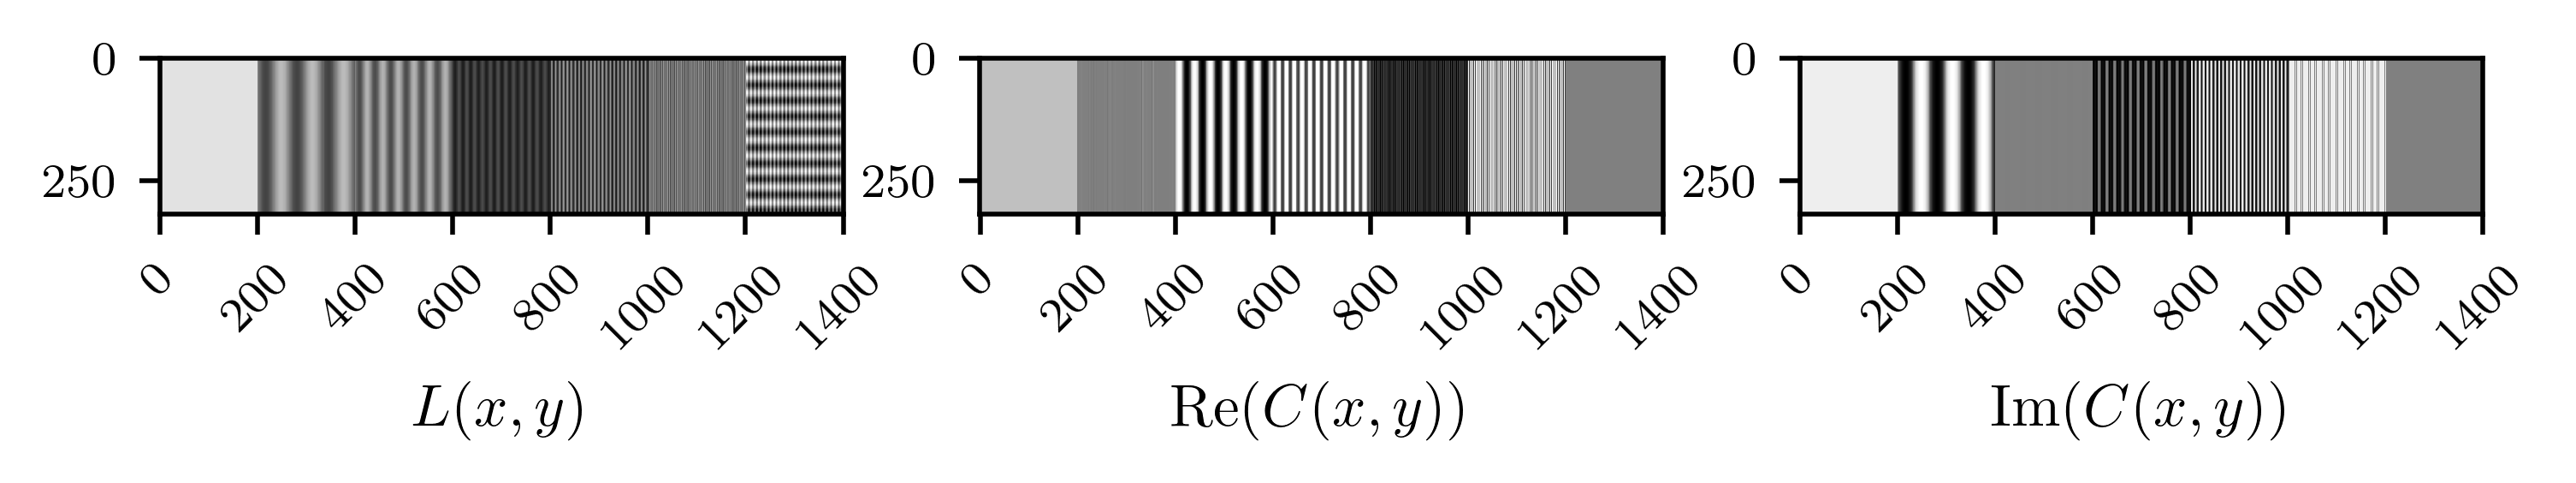
\includegraphics[width=0.5\textwidth]{synthetic_image_three_channel_decomposition}}
    \subcaptionbox{\label{fig:horizontal_line_three_channel_decomposition}}{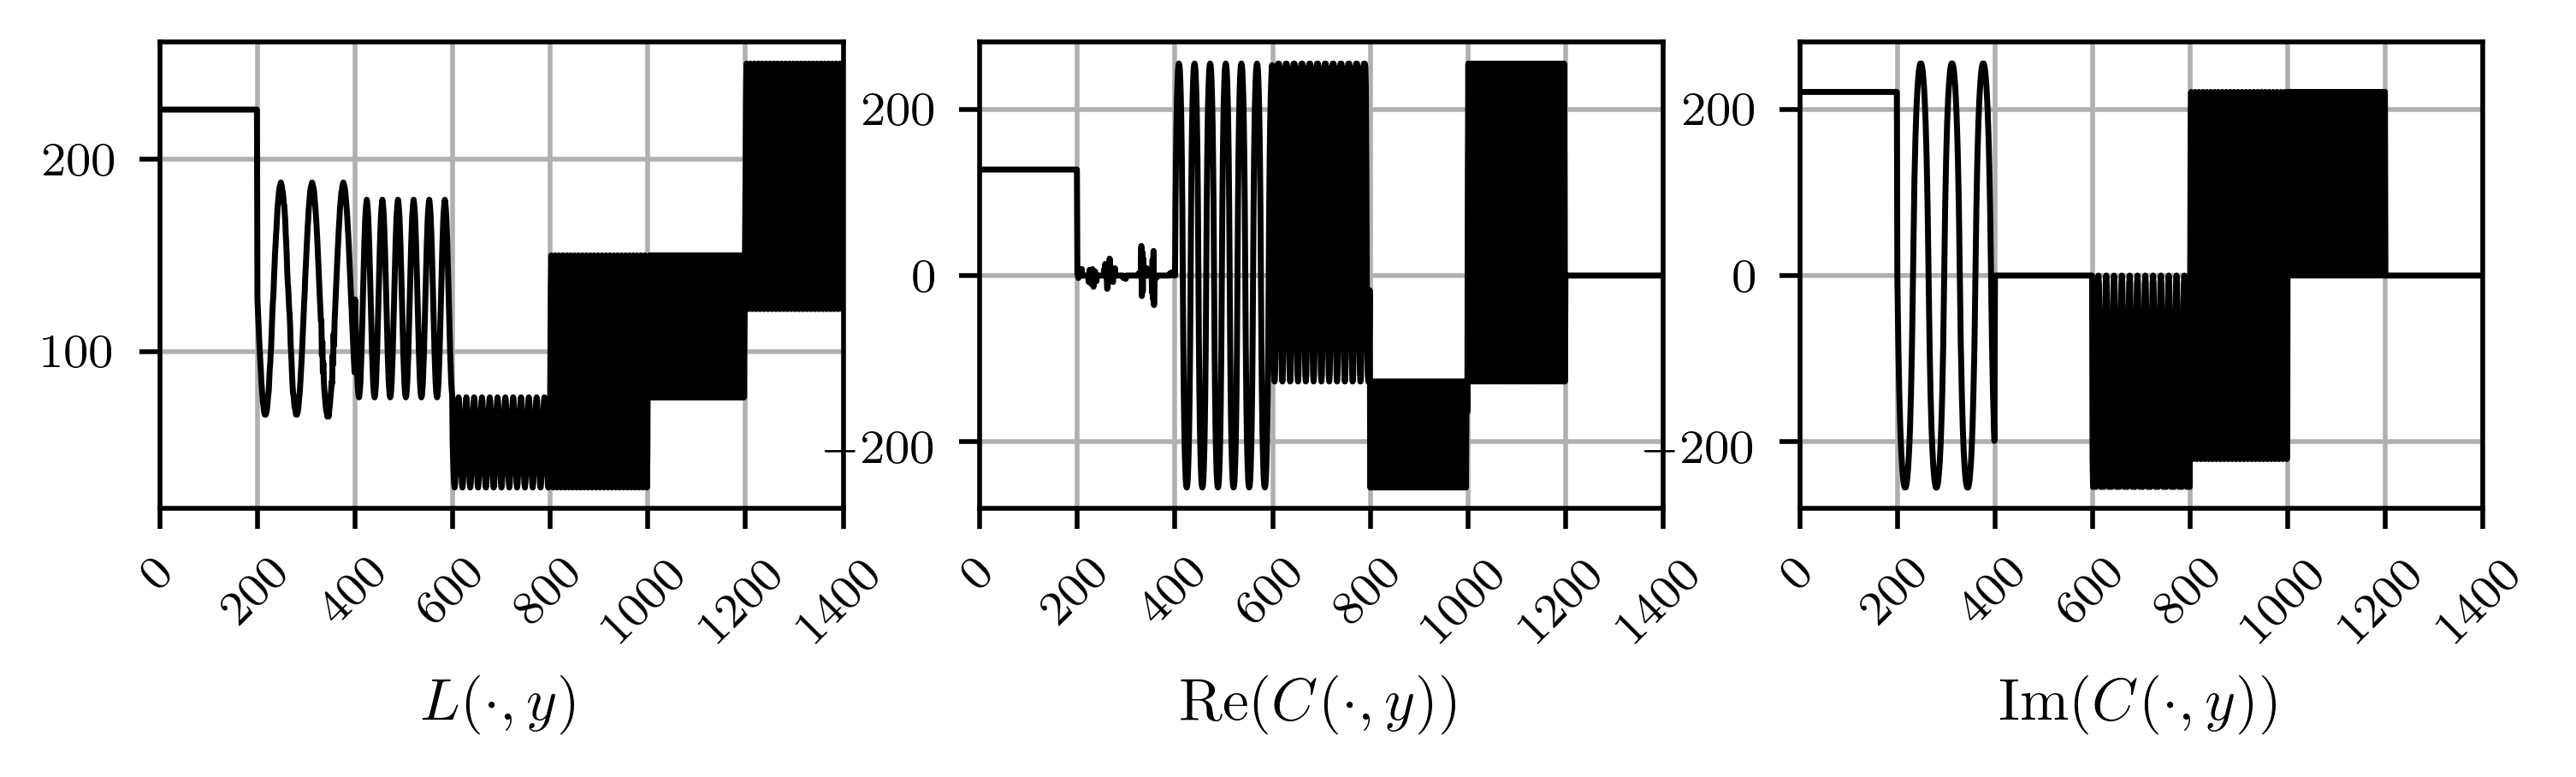
\includegraphics[width=0.5\textwidth]{horizontal_line_three_channel_decomposition}}    
\caption{Illustration of the proposed synthetic image: \captext{(a)} Luminance and chrominance decomposition; \captext{(b)} Numerical values on a horizontal line cut through the three channels.}\label{fig:three_channel_decomposition}
\end{figure}

\subsection{Feature Space Validation}

In this section, we integrate the feature space obtained with Gabor filters within a clustering framework. We hypothesize that if the color/texture features represent the variety of information in the images (synthetic and natural), we can obtain a consistent segmentation with this perceptual information. We then use the segmentation results to qualitatively and quantitatively evaluate our Gabor feature space.

Before clustering, we adapt the feature space to prepare it for the clustering methods.

\paragraph{Data organization}
The feature space 
\begin{equation}\label{eq:feature_space_clustering}
	X(x,y) = \widetilde{e}_{i, f, \theta}(x,y)
\end{equation}
is a log-polar space given the logarithmic scale of the $N$ frequencies and the $N$ orientations of the Gabor filter bank. Then, the feature space is composed of $3 \times M \times N$ Gabor responses, where the constant $3$ corresponds to the number of channels of the luminance-chrominance color space. We arrange the data to obtain a two-dimensional array of size $P \times D$, where $P= H\times W$  is the number of samples or pixels and $D =3 \times M \times N$ in the number of features or dimensions of the data.

\paragraph{Spatial information integration}
Gabor's color and texture features do not include spatial information. We enter such information by adding two more dimensions to the feature space $X$. These two features are the positional coordinates $(x, y)$ of each pixel in the image. 

\paragraph{Data standardization}
We standardize each feature $D$ of the $X$ matrix to have a mean of zero and a constant variance. We perform this operation to avoid the dominance of some features over others due to numerical differences of units of magnitude.

\paragraph{Dimensionality reduction}
We reduce the feature space's dimensions from $D =3 \times M \times N$ to $5$ using the linear transformation technique of principal component analysis (PCA). With the PCA we identify patterns in the feature space based on the correlation between features. We choose 5 as the new subspace dimension based on the idea that three of these dimensions contain Gabor's color and texture information, and the remaining two dimensions contain the spatial information. In addition, a low number of dimensions speeds up the calculation of clustering algorithms.

\subsection{Qualitative Evaluation}
We qualitatively validate the spectral decomposition of images based on Gabor filters for the generation of color texture features first, in fully controlled conditions using the synthetic image and later, with a semi-controlled set up using handmade texture mosaics.

In both cases, we use the k-means algorithm as a clustering method on the feature space $X$ setting the number of clusters manually. The grouping technique acts as a segmentation method, with which we validate our methodology.

\subsubsection{Synthetic Image Segmentation}
Looking at the synthetic image (Fig. \ref{fig:synthetic_color_texture_image}),  there are several coherent ways for a human observer to segment it. The two most apparent possibilities are to segment the image into 7 clusters, where each cluster represents a region of the image and; segment the image only into 2 clusters, where one cluster groups the regions with texture and the other the flat region. 

We apply these conditions to set the cluster's number of the k-means algorithm ($k = 7$ and $k = 2$) and obtain a segmentation of the synthetic image coherent with the human perception. The segmentation results are depicted in figure  \ref{fig:kmeans_segms_synthetic_img}. These segmentation results show that the Gabor multi-spectral analysis captures well the color and texture information. Also, the segmentation shows that both features (color and texture) are perceptually relevant in the image segmentation task.  

%\begin{figure}[!ht]
%    \centering
%    \begin{subfigure}[b]{\textwidth}
%        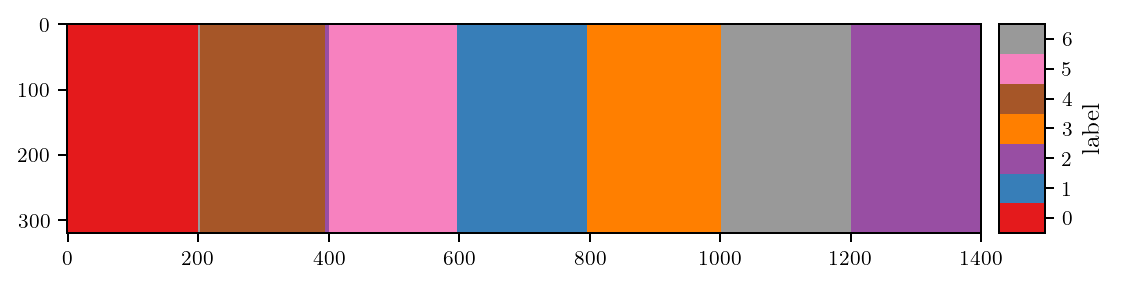
\includegraphics[width=0.5\textwidth]{kmeans_7segms_synthetic}
%        \caption{7 clusters segmentation}
%    \end{subfigure} \\    
%    \begin{subfigure}[b]{\textwidth}
%    	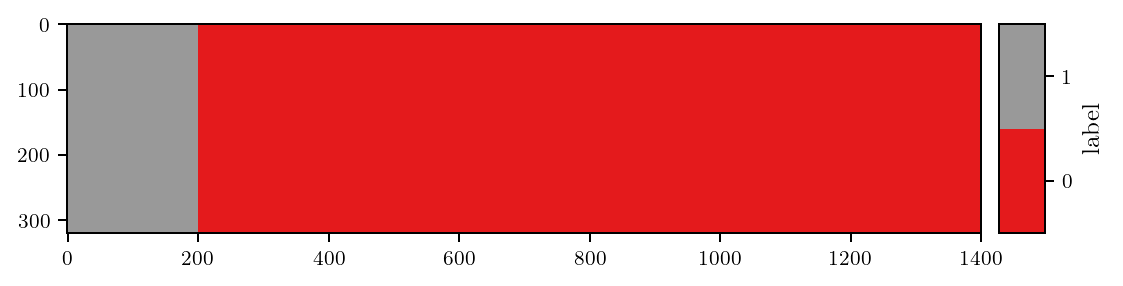
\includegraphics[width=0.5\textwidth]{kmeans_2segms_synthetic}
%        \caption{2 clusters segmentation}
%    \end{subfigure} 
%        	    
%    \caption{Synthetic image k-means segmentation results.}\label{fig:kmeans_segms_synthetic_img}    
%\end{figure}

\begin{figure*}[!t]
\centering
\subfloat[7 clusters segmentation]{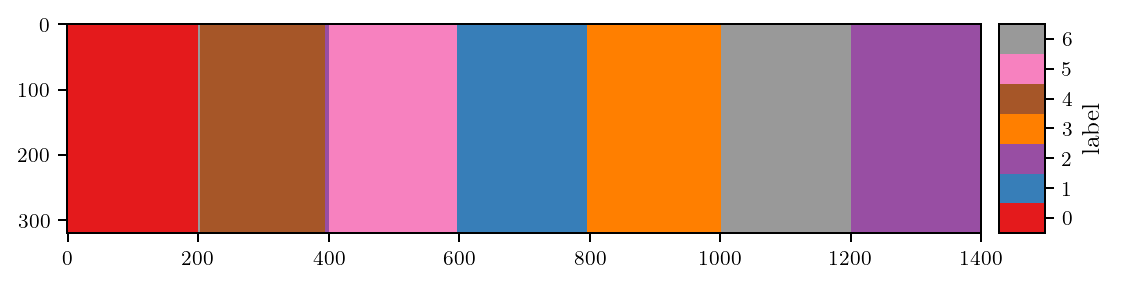
\includegraphics[width=0.5\textwidth]{kmeans_7segms_synthetic}%
}
\hfil
\subfloat[2 clusters segmentation]{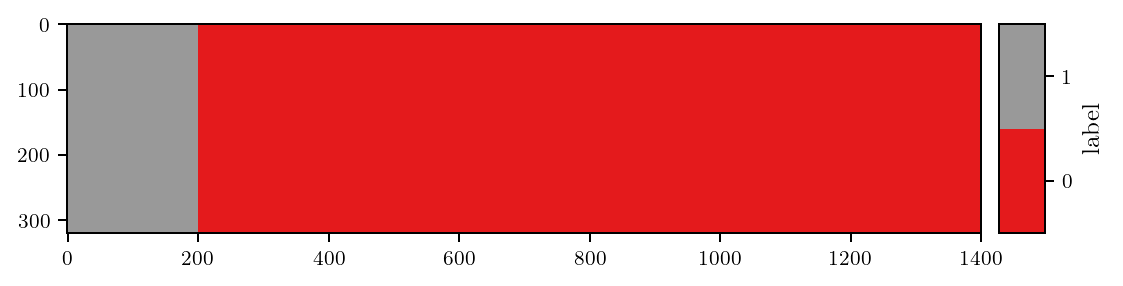
\includegraphics[width=0.5\textwidth]{kmeans_2segms_synthetic}%
}
\caption{Synthetic image k-means segmentation results.}\label{fig:kmeans_segms_synthetic_img}   
\end{figure*}

\subsubsection{DTD Mosaic Image Segmentation}
We go a step further and test our feature space under slightly more complex conditions; we created a series of color texture mosaics using images from the Describable Textures Dataset (DTD) \cite{Cimpoi.Maji.ea:CVPR:2014} as a base. The DTD is a collection of homogeneous nature textures with 47 annotated classes. To create the mosaics, we take 5 images of the same (or similar ) class and put them together in a collage. The five classes we take the images are \textit{lined-banded-zigzagged}, \textit{cracked}, \textit{braided}, \textit{dotted}, and \textit{striped-veined-scaly}. The texture collage we propose is relatively standard, with a circular patch in the center of the image that is superimposed on four square patches. 

We apply the clustering algorithm on each mosaic created, setting $ k = 5 $ clusters. The segmentation results are shown in figure \ref{fig:kmeans_segms_dtd_mosaics}. In this case, the clustering algorithm results are coherent with the input image; however, the segmentation's precision and quality are lower than in the synthetic image. This result is mainly due to the complexity of the natural textures in the mosaics. 

%\begin{figure}[!ht]
%    \centering
%    \begin{subfigure}[b]{0.19\textwidth}
%        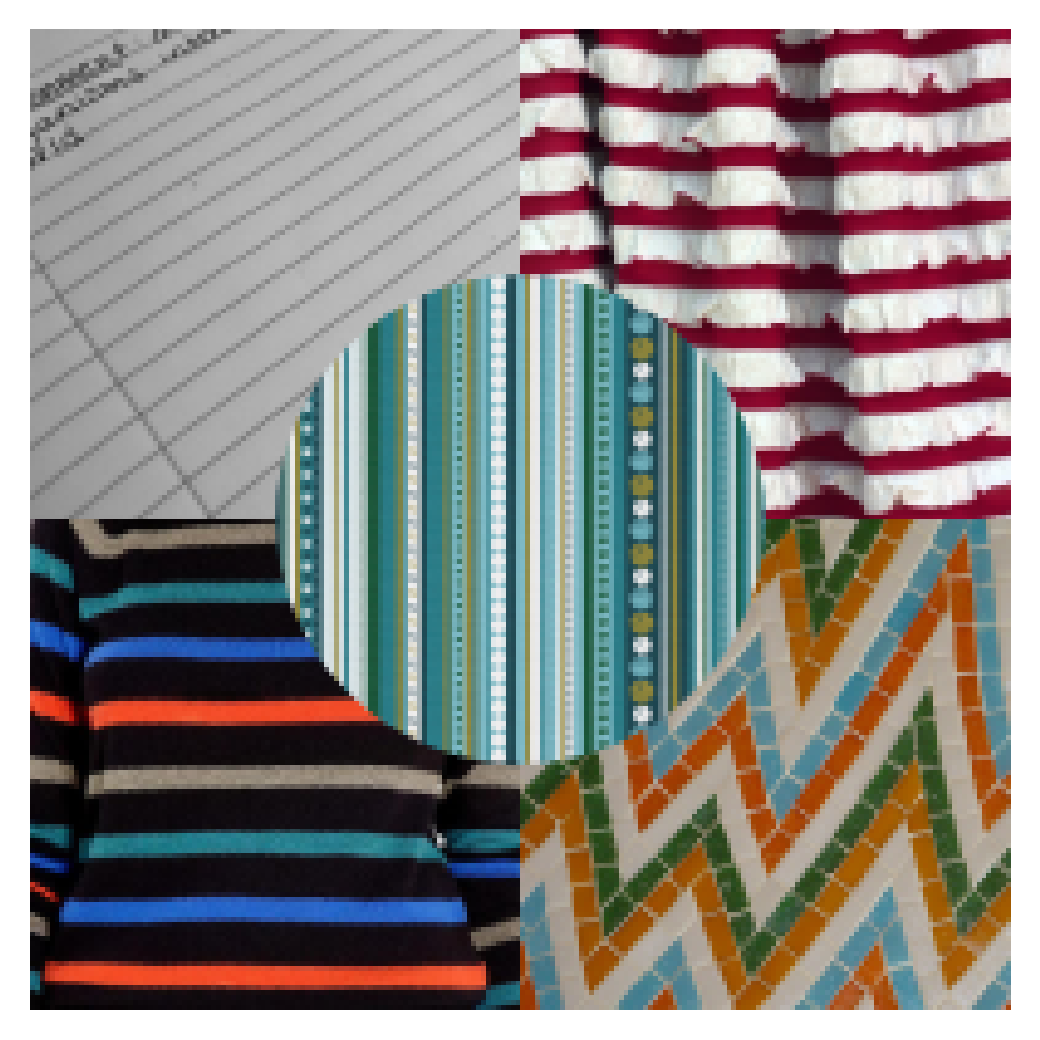
\includegraphics[width=\textwidth]{mosaic_dtd1}
%    \end{subfigure} 
%    \begin{subfigure}[b]{0.19\textwidth}
%    	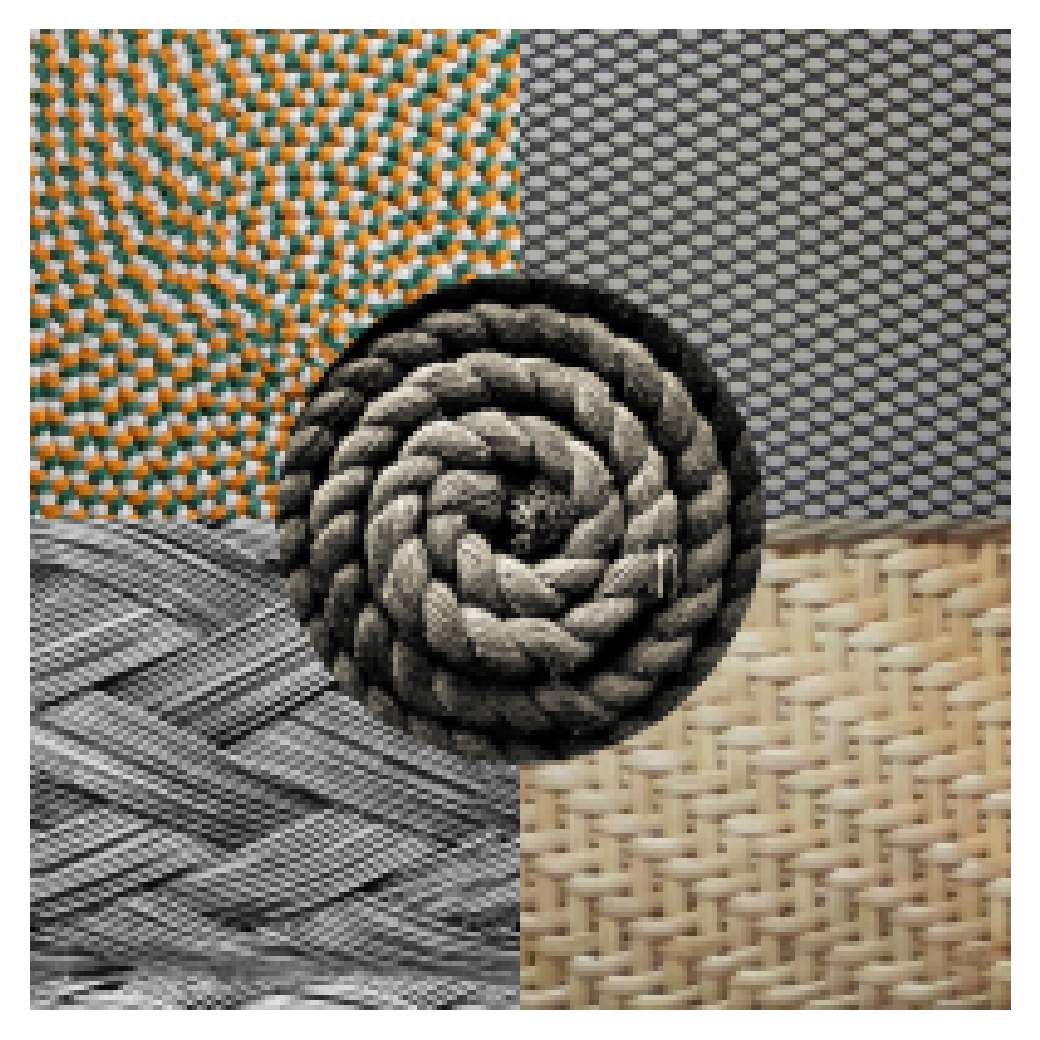
\includegraphics[width=\textwidth]{mosaic_dtd2}
%    \end{subfigure}     
%    \begin{subfigure}[b]{0.19\textwidth}
%        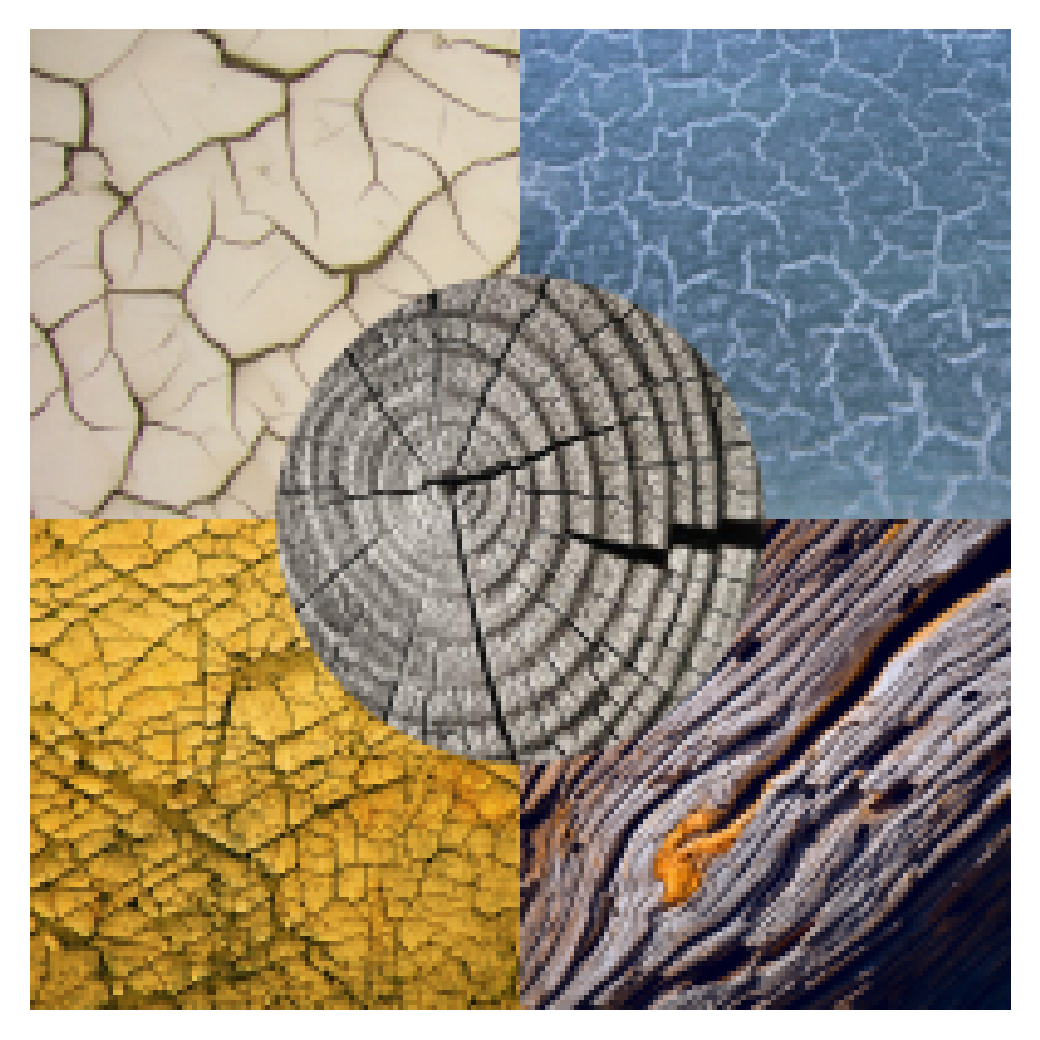
\includegraphics[width=\textwidth]{mosaic_dtd3}
%    \end{subfigure}
%    \begin{subfigure}[b]{0.19\textwidth}
%    	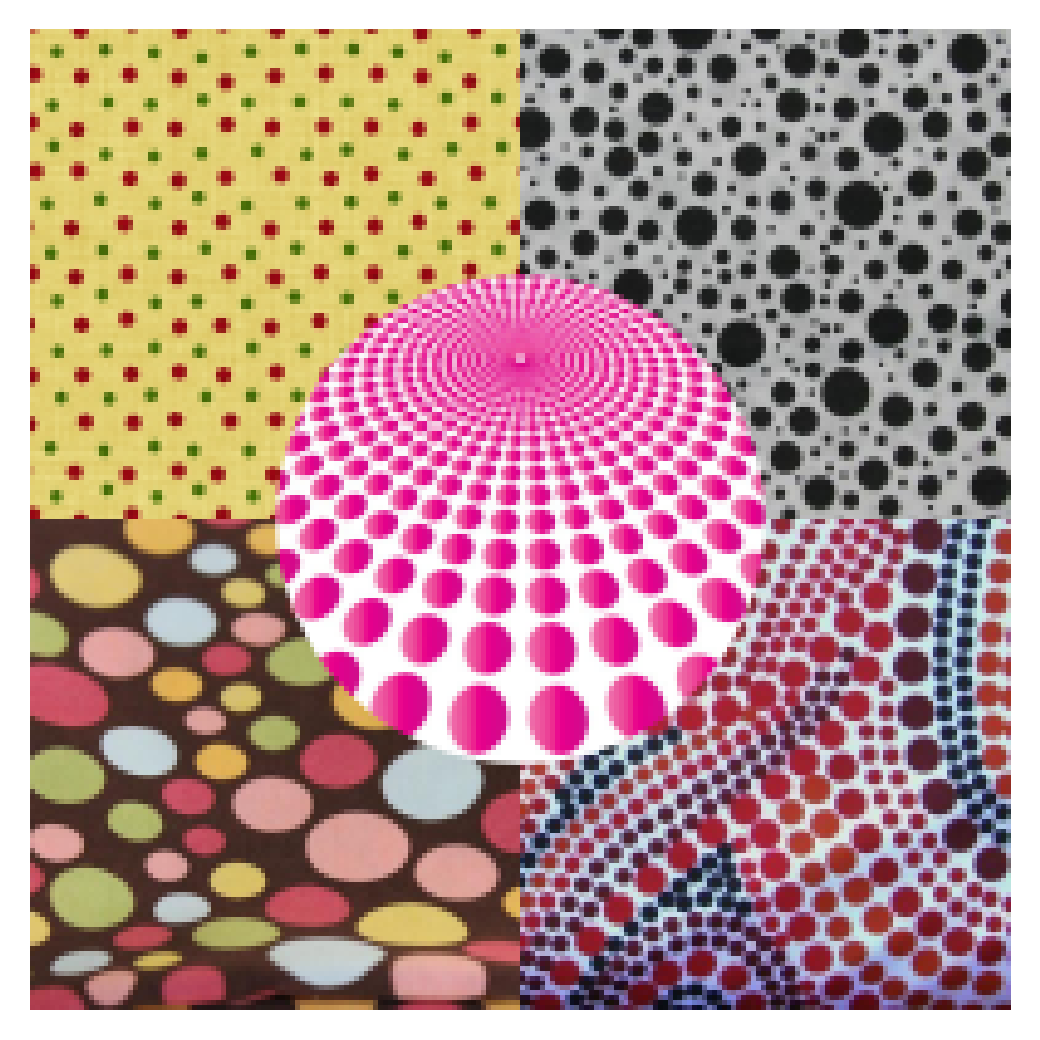
\includegraphics[width=\textwidth]{mosaic_dtd4}
%    \end{subfigure}    
%    \begin{subfigure}[b]{0.19\textwidth}
%        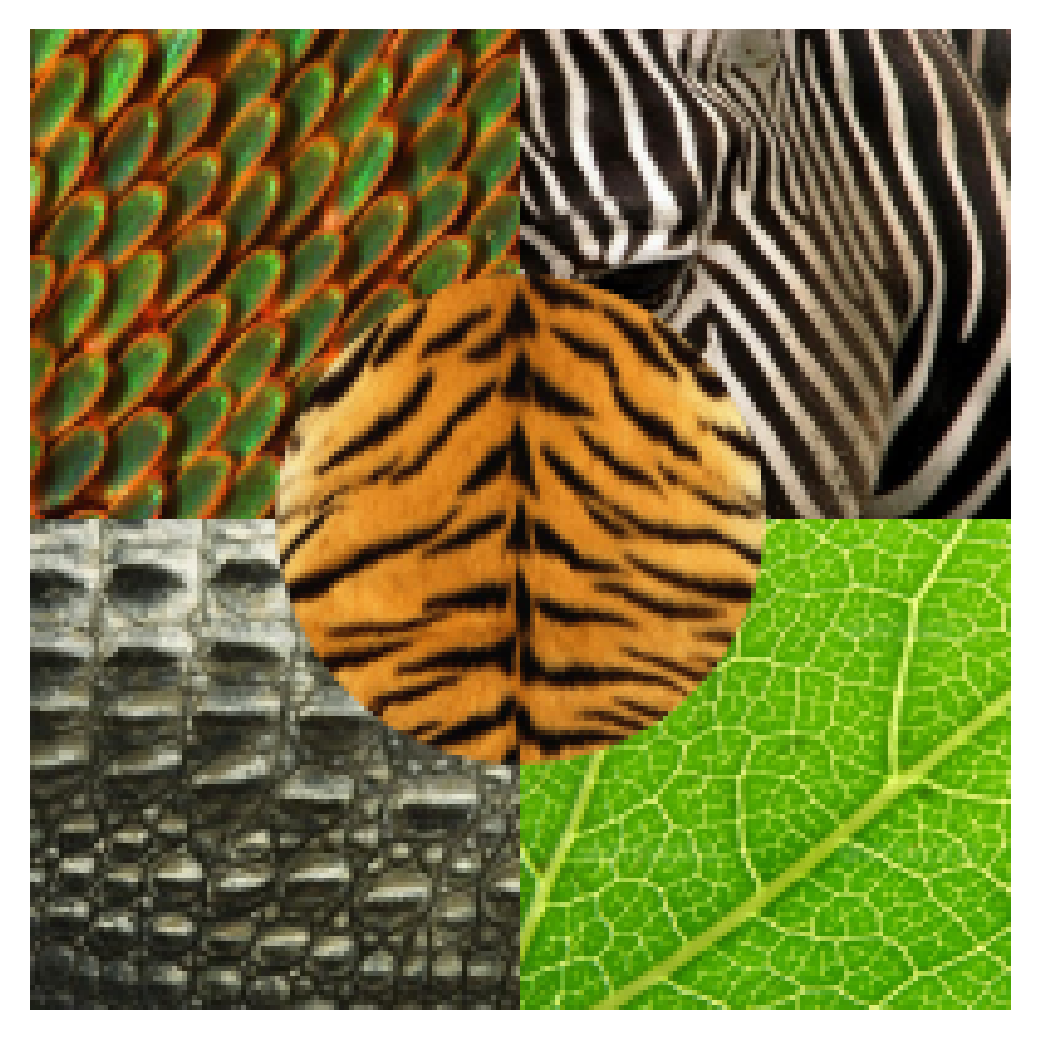
\includegraphics[width=\textwidth]{mosaic_dtd5}
%    \end{subfigure} \\ [2ex]
%    
%    \begin{subfigure}[b]{0.19\textwidth}
%    	
\includegraphics[width=\textwidth]{mosaic_dtd1_kmeans_segms}
%        \caption{}
%    \end{subfigure}     
%    \begin{subfigure}[b]{0.19\textwidth}
%        
\includegraphics[width=\textwidth]{mosaic_dtd2_kmeans_segms}
%        \caption{}
%    \end{subfigure} 
%    \begin{subfigure}[b]{0.19\textwidth}
%    	
\includegraphics[width=\textwidth]{mosaic_dtd3_kmeans_segms}
%        \caption{}
%    \end{subfigure}     
%    \begin{subfigure}[b]{0.19\textwidth}
%        
\includegraphics[width=\textwidth]{mosaic_dtd4_kmeans_segms}
%        \caption{}
%    \end{subfigure}
%    \begin{subfigure}[b]{0.19\textwidth}
%    	
\includegraphics[width=\textwidth]{mosaic_dtd5_kmeans_segms}
%        \caption{}
%    \end{subfigure} 
%        	    
%    \caption{DTD mosaics k-means segmentation results.}\label{fig:kmeans_segms_dtd_mosaics}    
%\end{figure}

\begin{figure*}[!t]
\centering
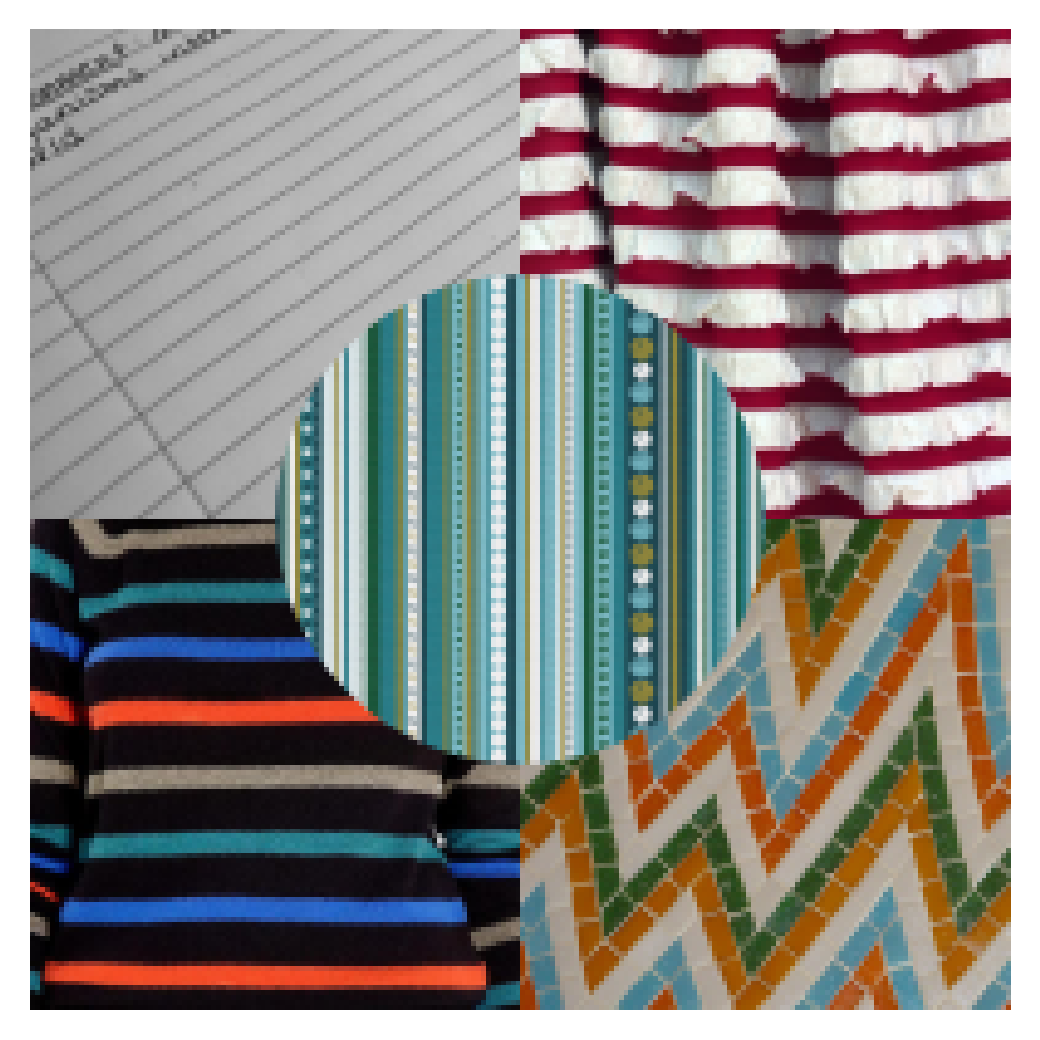
\includegraphics[width=0.13\textwidth]{mosaic_dtd1}\hfil
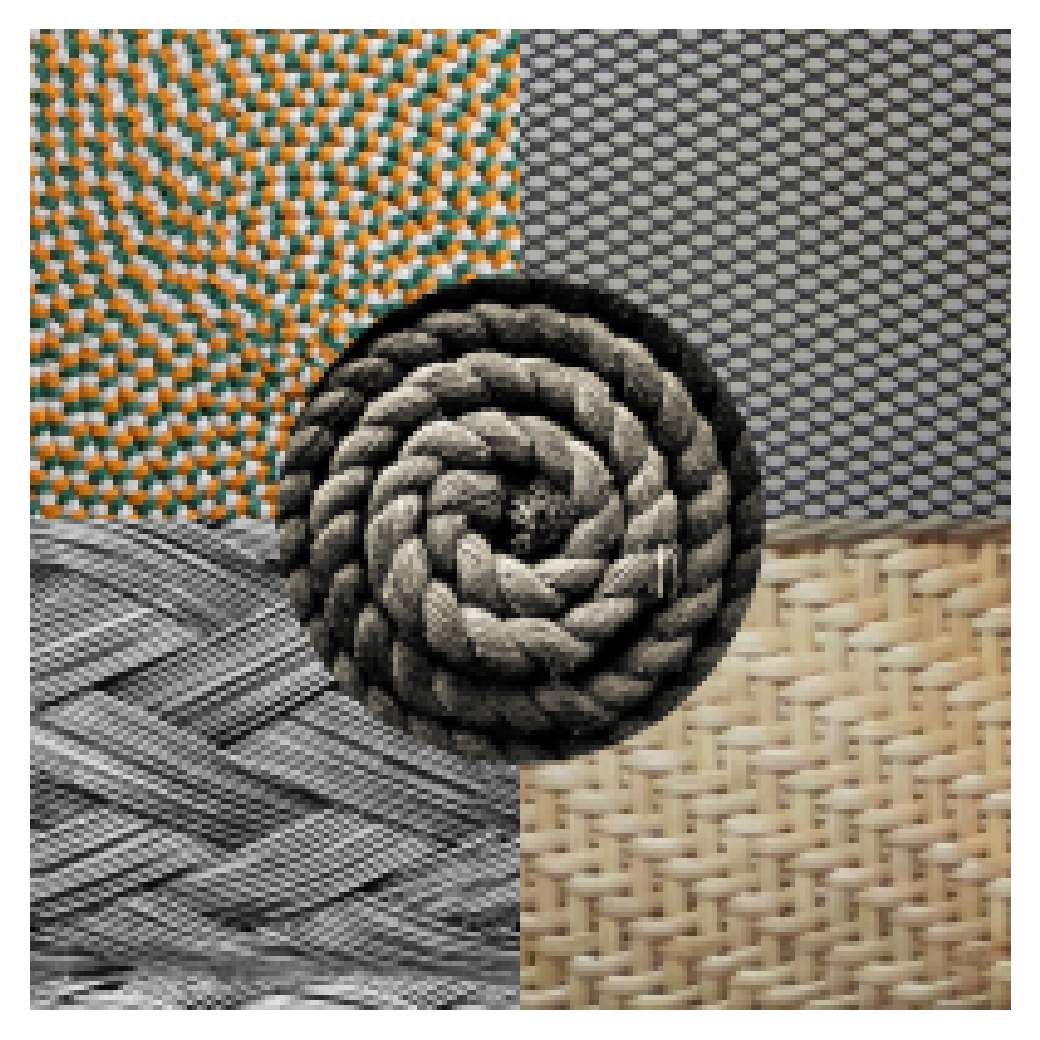
\includegraphics[width=0.13\textwidth]{mosaic_dtd2}\hfil
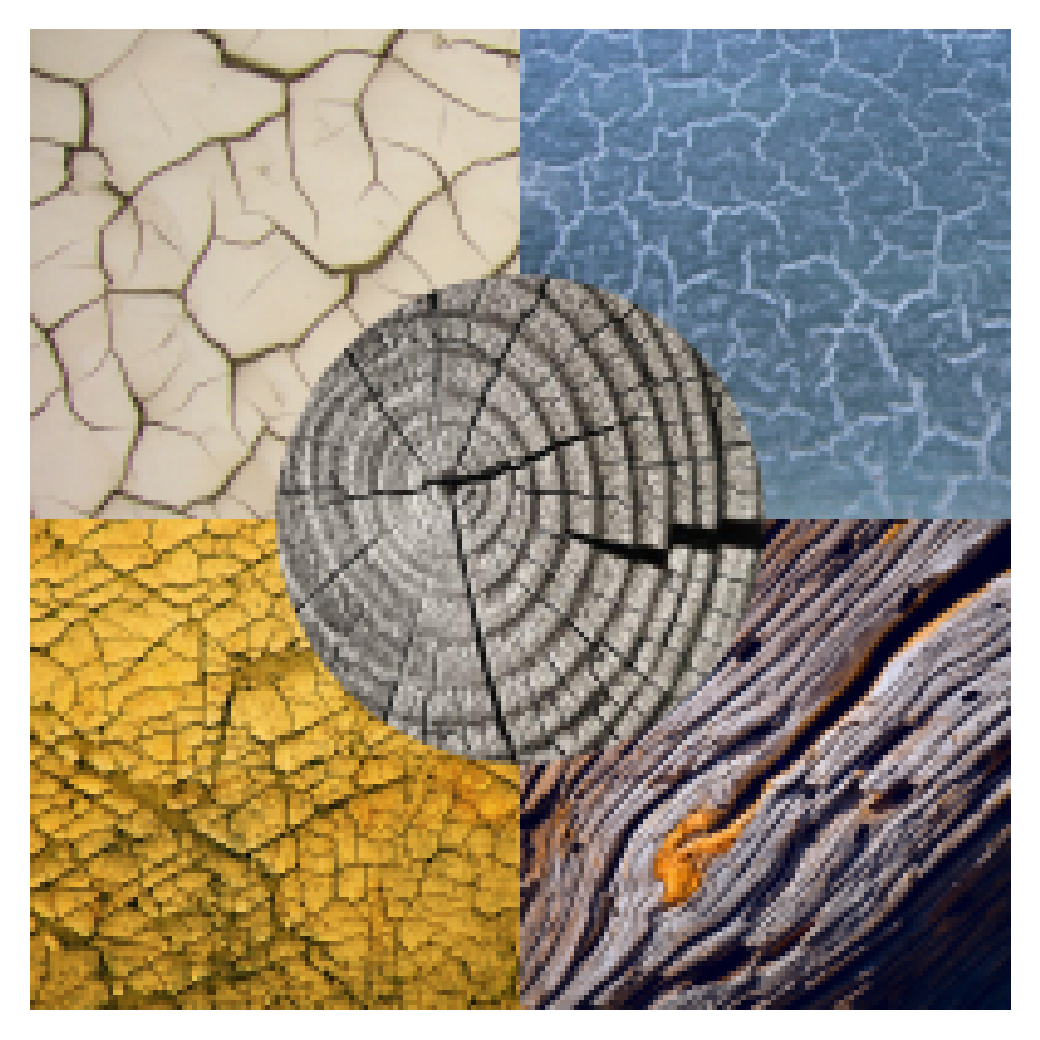
\includegraphics[width=0.13\textwidth]{mosaic_dtd3}\hfil
\includegraphics[width=0.13\textwidth]{mosaic_dtd4}\hfil
\includegraphics[width=0.13\textwidth]{mosaic_dtd5}\\[2ex]
\subfloat[]{\includegraphics[width=0.13\textwidth]{mosaic_dtd1_kmeans_segms}}\hfil
\subfloat[]{\includegraphics[width=0.13\textwidth]{mosaic_dtd2_kmeans_segms}}\hfil
\subfloat[]{\includegraphics[width=0.13\textwidth]{mosaic_dtd3_kmeans_segms}}\hfil
\subfloat[]{\includegraphics[width=0.13\textwidth]{mosaic_dtd4_kmeans_segms}}\hfil
\subfloat[]{\includegraphics[width=0.13\textwidth]{mosaic_dtd5_kmeans_segms}}
\caption{DTD mosaics k-means segmentation results.}\label{fig:kmeans_segms_dtd_mosaics}    
\end{figure*}

\subsection{Quantitative Evaluation}\label{subsec:quantitative_evaluation}

We also quantitatively evaluate the quality of the feature space developed in this chapter. For this, we use a database of natural images that have a ground truth generated by humans. The database and its characteristics are described below.

\subsubsection{Berkely Segmentation Image Data Set}
The Berkely Database for Segmentation (BSDS) is one of the gold standards for segmentation results \cite{Martin.Fowlkes.ea:ICCV:2001}. The BSDS comprises images from the Corel database selected under a simple criterion: choose images of complex and natural scenes containing at least one distinguishable object. Under this criteria, selected images contain multiple cues for human segmentation, for example, low-level cues such as coherence of brightness, texture, color, and contour continuity; mid-level cues such as symmetry, convexity, and area of the regions; as well as high-level cues based on the semantics of the image objects.

There are two versions of this database. The first one (BSDS300) contains 300 images, while the second (BSDS500) contains 500 images. Each image in the database contains between 5 and 11 human-made segmentations. The instruction given to the observers to naturally break the scene is simple:
\begin{displayquote}
Divide each image into pieces, where each piece represents a distinguished thing in the image. It is important that all of the pieces have approximately equal importance. The number of things in each image is up to you. Something between 2 and 30 should be reasonable for any of our images \cite{Martin.Fowlkes.ea:ICCV:2001}.
\end{displayquote}
Following these instructions, most segmentations meet the criterion of the number of segments; however, we can also find exceptions with more than 50 segmented things.

Finally, both databases (BSDS300 and BSDS500) contain segmentations of gray level and color images. Since in this chapter we analyze the color textures, we mainly use the BSDS500 color images with their respective segmentations to evaluate our segmentation results. Figure 3 shows some examples of images from the BSDS500 and the segmentations produced by different humans.

\subsubsection{Scores}
We use the human-generated segmentations of the BSDS500 as ground truth (GT), applying the precision-recall framework of \cite{Martin.Fowlkes.ea:PAMI:2004}. The precision is the fraction of detections that are true positives rather than false positives, while the recall is the fraction of true positives that are detected rather than missed. This evaluation framework is generally applied to evaluate contour detection algorithms. Therefore, applied in the image segmentation task, the framework involves evaluating the boundaries of the segmentation resulting regions, considering the detected boundaries pixels as a two-classes classification problem (contour and non-contour pixels). Under this configuration, precision is translated as the number of pixels correctly labeled as belonging to the contour class (true positives) divided by the total number of pixels labeled as contours (the sum of true positives and false positives). The recall in this context is defined as the number of true positives divided by the sum of true positives and the pixels which were not labeled as contours but should have been (false negatives). The following mathematical expressions define precision and recall.

\begin{equation}\label{eq:precision_score}
    \text{precision} = \frac{tp}{tp+fp}
\end{equation}

\begin{equation}\label{eq:recall_score}
    \text{recall} = \frac{tp}{tp+fn}
\end{equation}

A simple metric that captures the trade-off between precision and recall is the f-measure, which is defined as the harmonic mean between the two scores.

\begin{equation}\label{eq:f_score}
    \text{F-measure} = \frac{2 \times \text{precision}\times\text{recall}}{\text{precision} + \text{recall}}
\end{equation}


\subsubsection{Experiments Set up}

For the numerical evaluation, we perform the segmentation of the BSDS500 images using different clustering algorithms. In addition, we perform the segmentation in the feature space obtained with different luminance-chrominance color spaces, particularly those derived from the LAB, HSL, and HSV spaces. This series of experiments allows us to evaluate other aspects of our Gabor-based feature space, for example, the behavior of the feature space on different clustering algorithms (and vice-versa) and the performance of each clustering method in the image segmentation task. Other secondary items that we also analyze are the effect of the initial color space in the transformation to the two-channel color space, the effect of choosing the number of clusters to detect, and the computation time of the clustering algorithms. 

\paragraph{Clustering method vs. former luminance-chrominance color space.} 

Within the wide range of clustering algorithms that exist in the literature \cite{Omran.Engelbrecht.ea:IOS:2007} \cite{Sathya.Manavalan:IJCA:2011}, we performed the segmentation of the BSDS images using four different clustering techniques: k-means, fast k-means, Birch, and Gaussian mixture. The choice of these techniques depends on the characteristics of the input data: a high dimensional space with a large number of observations. Such input data comes from the multi-spectral decomposition of the images using Gabor filters on the luminance-chrominance channels of the images. We then compare the performance of the different clustering algorithms on the luminance-chrominance feature spaces from the HSV, HSL, and LAB color spaces reviewed in chapter \ref{ch:color_texure_representations}. 

Figures \ref{fig:lynx_clustering_method_v_colorspace} and \ref{fig:pheasant_clustering_method_v_colorspace} show the segmentation results of two BSDS500 images. In both cases, the images contain wild animals in their natural environment, which implies that the color and texture of the fur/feathers create a mimicry that helps the animals to blend in with the scene. Animal mimicry makes segmentation a challenging problem. Despite this, we see how some configurations of color space and clustering algorithms manage to classify the pixels based on the perceptual information of color and texture encoded on the Gabor features. Particularly in these two segmentation examples, we could say that the color space that best represents the color and texture information of the image is the HSL, while the clustering method that best uses the multi-spectral features is the Gaussian mixture. 

For the segmentation results shown in Figures \ref{fig:lynx_clustering_method_v_colorspace} and \ref{fig:pheasant_clustering_method_v_colorspace}, we use $k = 4$ as the target number of clusters to find in the image. In addition, for visualization purposes, we display the resulting clusters with the mean color of the pixels of the original image within the segmentation regions. 

\begin{figure*}[!t]
         
    \begin{subfigure}[b]{\dimexpr0.23\textwidth+20pt\relax}
    	\centering
    	\makebox[20pt]{\raisebox{30pt}{ \rotatebox[origin=c]{90} {\small \textsf{\textbf{Input image}}} }}%
    	\includegraphics[width=\dimexpr\linewidth-20pt\relax]{160067} 
    \end{subfigure}  \\ \vspace{-5pt}    
    
    
    \begin{subfigure}[b]{\dimexpr0.23\textwidth+20pt\relax}
    	\centering
    	\makebox[20pt]{\raisebox{30pt}{ \rotatebox[origin=c]{90} {\small \textsf{\textbf{LAB}}} }}%
    	\includegraphics[width=\dimexpr\linewidth-20pt\relax]{160067_KMeans_const_segm_HSV} 
    \end{subfigure}      
%    ~ %add desired spacing between images, e. g. ~, \quad, \qquad, \hfill etc. 
      %(or a blank line to force the subfigure onto a new line)
    \begin{subfigure}[b]{0.23\textwidth}
    	\centering
        \includegraphics[height=67.68857pt]{160067_MiniBatchKMeans_const_segm_HSV}
    \end{subfigure}
%    ~ %add desired spacing between images, e. g. ~, \quad, \qquad, \hfill etc. 
      %(or a blank line to force the subfigure onto a new line)
    \begin{subfigure}[b]{0.23\textwidth}
    	\centering
        \includegraphics[height=67.68857pt]{160067_Birch_const_segm_LAB}
    \end{subfigure}
%    ~ %add desired spacing between images, e. g. ~, \quad, \qquad, \hfill etc. 
      %(or a blank line to force the subfigure onto a new line)
    \begin{subfigure}[b]{0.23\textwidth}
    	\centering
        \includegraphics[height=67.68857pt]{160067_GaussianMixture_const_segm_HSV}
    \end{subfigure} \\ \vspace{-5pt}  
    
          
    \begin{subfigure}[b]{\dimexpr0.23\textwidth+20pt\relax}
    	\centering
    	\makebox[20pt]{\raisebox{30pt}{ \rotatebox[origin=c]{90} {\small \textsf{\textbf{HSV}}} }}%
    	\includegraphics[width=\dimexpr\linewidth-20pt\relax]{160067_KMeans_const_segm_LAB} 
    \end{subfigure}      
%    ~ %add desired spacing between images, e. g. ~, \quad, \qquad, \hfill etc. 
      %(or a blank line to force the subfigure onto a new line)
    \begin{subfigure}[b]{0.23\textwidth}
    	\centering
        \includegraphics[height=67.68857pt]{160067_MiniBatchKMeans_const_segm_LAB}
    \end{subfigure}
%    ~ %add desired spacing between images, e. g. ~, \quad, \qquad, \hfill etc. 
      %(or a blank line to force the subfigure onto a new line)
    \begin{subfigure}[b]{0.23\textwidth}
    	\centering
        \includegraphics[height=67.68857pt]{160067_Birch_const_segm_LAB}
    \end{subfigure}
%    ~ %add desired spacing between images, e. g. ~, \quad, \qquad, \hfill etc. 
      %(or a blank line to force the subfigure onto a new line)
    \begin{subfigure}[b]{0.23\textwidth}
    	\centering
        \includegraphics[height=67.68857pt]{160067_GaussianMixture_const_segm_HSV}
    \end{subfigure} \\ \vspace{-5pt}
    
           
    \begin{subfigure}[b]{\dimexpr0.23\textwidth+20pt\relax}
    	\centering
    	\makebox[20pt]{\raisebox{30pt}{ \rotatebox[origin=c]{90} {\small \textsf{\textbf{HSL}}} }}%
    	\includegraphics[width=\dimexpr\linewidth-20pt\relax]{160067_KMeans_const_segm_HSL} 
    	\caption{k-means}
    \end{subfigure}      
%    ~ %add desired spacing between images, e. g. ~, \quad, \qquad, \hfill etc. 
      %(or a blank line to force the subfigure onto a new line)
    \begin{subfigure}[b]{0.23\textwidth}
    	\centering
        \includegraphics[height=67.68857pt]{160067_MiniBatchKMeans_const_segm_HSL}
        \caption{Fast k-means}
    \end{subfigure}
%    ~ %add desired spacing between images, e. g. ~, \quad, \qquad, \hfill etc. 
      %(or a blank line to force the subfigure onto a new line)
    \begin{subfigure}[b]{0.23\textwidth}
    	\centering
        \includegraphics[height=67.68857pt]{160067_Birch_const_segm_HSL}
        \caption{Birch}
    \end{subfigure}
%    ~ %add desired spacing between images, e. g. ~, \quad, \qquad, \hfill etc. 
      %(or a blank line to force the subfigure onto a new line)
    \begin{subfigure}[b]{0.23\textwidth}
    	\centering
        \includegraphics[height=67.68857pt]{160067_GaussianMixture_const_segm_HSL}
        \caption{Gaussian mixture}
    \end{subfigure} 
    
	\caption{Importance of the color space and the clustering algorithm in the image segmentation task using the feature space based on Gabor filters. BSDS lynx image segmentation results.}\label{fig:lynx_clustering_method_v_colorspace}    
\end{figure*}

\paragraph{Number of clusters in the data.} 
Determining the number of segments to detect when using clustering algorithms as an image segmentation technique is a frequent problem. The four algorithms we present here for image segmentation need the $k$ parameter to specify the number of clusters to find. Although there are techniques to estimate the number of regions in the image, these strategies involve one more stage of processing, which is reflected in the final segmentation calculation time. To find the optimal number of regions, we use the GT of the BSDS500. Since each image in the database contains between 5 and 11 human-made segmentations $\mathcal{S}=\{\mathcal{S}_1, \mathcal{S}_1, \cdots, \mathcal{S}_n\}$, we take $k$ as the maximum and the minimum number of segments found by the human observers for each image. 
\begin{eqnarray}
	k = \mathrm{max}(\mathcal{S}) \\
	k = \mathrm{min}(\mathcal{S})
\end{eqnarray}

Figure \ref{fig:Gmixture_starfish_segms_diff_k} shows the segmentation result of a BSDS image by manually setting $k$ with fixed values of 3 and 4 segments and defining $k$ as the number of maximum and minimum segments of the GT. In this particular case of the starfish image, the maximum number of annotated segments by a human observer is 92, while the minimum number of annotated segments is 6. The clustering algorithm used for this experiment is the Gaussian mixture in using the feature space from the LAB color space.


\begin{figure*}[!t]
    
    \begin{subfigure}[b]{0.18\textwidth}
    	\centering
        \includegraphics[width=\textwidth]{12003}
        \caption{Input image}
    \end{subfigure} ~    
    \begin{subfigure}[b]{0.18\textwidth}
    	\centering
    	\includegraphics[width=\textwidth]{12003_GaussianMixture_3_segm}
        \caption{$k=3$ }
    \end{subfigure} ~
    \begin{subfigure}[b]{0.18\textwidth}
    	\centering
        \includegraphics[width=\textwidth]{12003_GaussianMixture_4_segm}
        \caption{$k=4$}
    \end{subfigure} ~
    \begin{subfigure}[b]{0.18\textwidth}
    	\centering
    	\includegraphics[width=\textwidth]{12003_GaussianMixture_min_segm}
        \caption{$k=\mathrm{min}(\mathcal{S})$}
    \end{subfigure} ~
    \begin{subfigure}[b]{0.18\textwidth}
    	\centering
    	\includegraphics[width=\textwidth]{12003_GaussianMixture_max_segm}
        \caption{$k=\mathrm{max}(\mathcal{S})$}
    \end{subfigure} 
        	    
    \caption{Effect of the choice of the number of clusters $k$ in clustering algorithms as segmentation methods.}\label{fig:Gmixture_starfish_segms_diff_k}    
\end{figure*}

The image segmentation results show various phenomena. The first one is the big difference between human-made segmentations; the annotation with 92 regions implies a very detailed segmentation, while the annotation with 6 regions does not reflect the most basic segmentation of the image: two objects, the starfish and the background. Both of these extrema, despite their substantial difference, are considered as ground truth.

This behavior is of vital importance in evaluating a segmentation algorithm since the scores are a function of the GT. In the case of the BSDS500, increasing $k$ means finding more regions that coincide with the GT regions, so the recall score increases; however, the precision of the regions found is very low. On the other hand, by decreasing, $k$ we detect fewer regions, which favors the precision score but affects the recall. Figure \ref{fig:PR_boxplot_scores_min_max_clusters} shows this phenomenon with the boxplots of the precision and recall scores of the different clustering methods using $k = \mathrm{min}(\mathcal{S})$ and $k = \mathrm{max}(\mathcal{S})$. Therefore, the optimal number of clusters $k$ should keep a balance between maximum data compression using a single cluster and maximum precision when assigning each pixel to its own cluster.

\begin{figure}[!t]
    \centering
    \begin{subfigure}[b]{0.24\textwidth}
        \includegraphics[width=\textwidth]{PrecisionRecall_boxplot_min_nclusters_LAB}
        \caption{$k=\mathrm{min}(\mathcal{S})$}
    \end{subfigure}   
    \begin{subfigure}[b]{0.24\textwidth}
    	\centering
    	\includegraphics[width=\textwidth]{PrecisionRecall_boxplot_max_nclusters_LAB}
        \caption{$k=\mathrm{max}(\mathcal{S})$}
    \end{subfigure}     
            	    
    \caption{Synthetic image k-means segmentation results.}\label{fig:PR_boxplot_scores_min_max_clusters}    
\end{figure}
\subsubsection{Results}
The two previous experiments show that the segmentation of real images is a complex task in which the result depends on various parameters such as the configuration of the input space, the number of segments, etc. Here we show some segmentation results (see figure \ref{fig:BSD_clustering_results}) using the feature space derived from the HSV-based luminance-chrominance color space and the four segmentation algorithms presented in this section.

The segmentation results are obtained by setting $k = 4$ for all images. Figure \ref{fig:PR_boxplot_scores} shows the precision and recall boxplots of each segmentation algorithm using the three different color spaces (HSV, HSL, and LAB).

\begin{figure*}[!t]
    \centering
    \begin{subfigure}[b]{0.30\textwidth}
        \includegraphics[width=\textwidth]{PrecisionRecall_boxplot_const_nclusters_HSL}
        \caption{HSL}
    \end{subfigure}\hfill 
    \begin{subfigure}[b]{0.30\textwidth}
    	\centering
    	\includegraphics[width=\textwidth]{PrecisionRecall_boxplot_const_nclusters_HSV}
        \caption{HSV}
    \end{subfigure}\hfill     
    \begin{subfigure}[b]{0.30\textwidth}
    	\centering
        \includegraphics[width=\textwidth]{PrecisionRecall_boxplot_const_nclusters_LAB}
        \caption{LAB}
    \end{subfigure} 
        	    
    \caption{Boxplots of precision and recall scores of the different clustering methods and the different color spaces. For the three plots, the number of clusters was set constant at $k=4$.}\label{fig:PR_boxplot_scores}    
\end{figure*}


\begin{figure*}[!ht]
         
    \begin{subfigure}[t]{\dimexpr0.23\textwidth+20pt\relax}
    	\centering
    	\makebox[20pt]{\raisebox{30pt}{ \rotatebox[origin=c]{90} {\small \textsf{\textbf{Input image}}} }}%
    	\includegraphics[width=\dimexpr\linewidth-20pt\relax]{100007} 
    \end{subfigure}      
%    ~ %add desired spacing between images, e. g. ~, \quad, \qquad, \hfill etc. 
      %(or a blank line to force the subfigure onto a new line)
    \begin{subfigure}[b]{0.23\textwidth}
    	\centering
        \includegraphics[height=67.68857pt]{101084}
    \end{subfigure}
%    ~ %add desired spacing between images, e. g. ~, \quad, \qquad, \hfill etc. 
      %(or a blank line to force the subfigure onto a new line)
    \begin{subfigure}[b]{0.23\textwidth}
    	\centering
        \includegraphics[height=67.68857pt]{175083}
    \end{subfigure}
%    ~ %add desired spacing between images, e. g. ~, \quad, \qquad, \hfill etc. 
      %(or a blank line to force the subfigure onto a new line)
    \begin{subfigure}[b]{0.23\textwidth}
    	\centering
        \includegraphics[height=67.68857pt]{181021}
    \end{subfigure} \\ 
    
    \begin{subfigure}[t]{\dimexpr0.23\textwidth+20pt\relax}
    	\centering
    	\makebox[20pt]{\raisebox{30pt}{ \rotatebox[origin=c]{90} {\small \textsf{\textbf{Kmeans}}} }}%
    	\includegraphics[width=\dimexpr\linewidth-20pt\relax]{100007_Kmeans_const_segm} 
    \end{subfigure}      
%    ~ %add desired spacing between images, e. g. ~, \quad, \qquad, \hfill etc. 
      %(or a blank line to force the subfigure onto a new line)
    \begin{subfigure}[b]{0.23\textwidth}
    	\centering
        \includegraphics[height=67.68857pt]{101084_Kmeans_const_segm}
    \end{subfigure}
%    ~ %add desired spacing between images, e. g. ~, \quad, \qquad, \hfill etc. 
      %(or a blank line to force the subfigure onto a new line)
    \begin{subfigure}[b]{0.23\textwidth}
    	\centering
        \includegraphics[height=67.68857pt]{175083_Kmeans_const_segm}
    \end{subfigure}
%    ~ %add desired spacing between images, e. g. ~, \quad, \qquad, \hfill etc. 
      %(or a blank line to force the subfigure onto a new line)
    \begin{subfigure}[b]{0.23\textwidth}
    	\centering
        \includegraphics[height=67.68857pt]{181021_Kmeans_const_segm}
    \end{subfigure} \\ 
       
    \begin{subfigure}[t]{\dimexpr0.23\textwidth+20pt\relax}
    	\centering
    	\makebox[20pt]{\raisebox{30pt}{ \rotatebox[origin=c]{90} {\small \textsf{\textbf{Fast Kmeans}}} }}%
    	\includegraphics[width=\dimexpr\linewidth-20pt\relax]{100007_MiniBatchKMeans_const_segm} 
    \end{subfigure}      
%    ~ %add desired spacing between images, e. g. ~, \quad, \qquad, \hfill etc. 
      %(or a blank line to force the subfigure onto a new line)
    \begin{subfigure}[b]{0.23\textwidth}
    	\centering
        \includegraphics[height=67.68857pt]{101084_MiniBatchKMeans_const_segm}
    \end{subfigure}
%    ~ %add desired spacing between images, e. g. ~, \quad, \qquad, \hfill etc. 
      %(or a blank line to force the subfigure onto a new line)
    \begin{subfigure}[b]{0.23\textwidth}
    	\centering
        \includegraphics[height=67.68857pt]{175083_MiniBatchKMeans_const_segm}
    \end{subfigure}
%    ~ %add desired spacing between images, e. g. ~, \quad, \qquad, \hfill etc. 
      %(or a blank line to force the subfigure onto a new line)
    \begin{subfigure}[b]{0.23\textwidth}
    	\centering
        \includegraphics[height=67.68857pt]{181021_MiniBatchKMeans_const_segm}
    \end{subfigure} \\ 
    
    \begin{subfigure}[t]{\dimexpr0.23\textwidth+20pt\relax}
    	\centering
    	\makebox[20pt]{\raisebox{30pt}{ \rotatebox[origin=c]{90} {\small \textsf{\textbf{Guassian mixture}}} }}%
    	\includegraphics[width=\dimexpr\linewidth-20pt\relax]{100007_GaussianMixture_const_segm} 
    \end{subfigure}      
%    ~ %add desired spacing between images, e. g. ~, \quad, \qquad, \hfill etc. 
      %(or a blank line to force the subfigure onto a new line)
    \begin{subfigure}[b]{0.23\textwidth}
    	\centering
        \includegraphics[height=67.68857pt]{101084_GaussianMixture_const_segm}
    \end{subfigure}
%    ~ %add desired spacing between images, e. g. ~, \quad, \qquad, \hfill etc. 
      %(or a blank line to force the subfigure onto a new line)
    \begin{subfigure}[b]{0.23\textwidth}
    	\centering
        \includegraphics[height=67.68857pt]{175083_GaussianMixture_const_segm}
    \end{subfigure}
%    ~ %add desired spacing between images, e. g. ~, \quad, \qquad, \hfill etc. 
      %(or a blank line to force the subfigure onto a new line)
    \begin{subfigure}[b]{0.23\textwidth}
    	\centering
        \includegraphics[height=67.68857pt]{181021_GaussianMixture_const_segm}
    \end{subfigure} \\ 
    
    \begin{subfigure}[t]{\dimexpr0.23\textwidth+20pt\relax}
    	\centering
    	\makebox[20pt]{\raisebox{30pt}{ \rotatebox[origin=c]{90} {\small \textsf{\textbf{Birch}}} }}%
    	\includegraphics[width=\dimexpr\linewidth-20pt\relax]{100007_Birch_const_segm} 
    \end{subfigure}      
%    ~ %add desired spacing between images, e. g. ~, \quad, \qquad, \hfill etc. 
      %(or a blank line to force the subfigure onto a new line)
    \begin{subfigure}[b]{0.23\textwidth}
    	\centering
        \includegraphics[height=67.68857pt]{101084_Birch_const_segm}
    \end{subfigure}
%    ~ %add desired spacing between images, e. g. ~, \quad, \qquad, \hfill etc. 
      %(or a blank line to force the subfigure onto a new line)
    \begin{subfigure}[b]{0.23\textwidth}
    	\centering
        \includegraphics[height=67.68857pt]{175083_Birch_const_segm}
    \end{subfigure}
%    ~ %add desired spacing between images, e. g. ~, \quad, \qquad, \hfill etc. 
      %(or a blank line to force the subfigure onto a new line)
    \begin{subfigure}[b]{0.23\textwidth}
    	\centering
        \includegraphics[height=67.68857pt]{181021_Birch_const_segm}
    \end{subfigure}     
	\caption{Segmentation results using different segmentation algorithms and HSV color space. The number of segments to find is fixed at $ k = 4 $ for all images. }\label{fig:BSD_clustering_results}    
\end{figure*}

\subsection{High-level Texture Features}\label{sec:high_level_features}
This section addresses the methodology for the extraction of high-level local texture features. To this end, we base the study of image textures on the Gabor filters. We obtain a spectral decomposition of the image through the convolution of the image with the filter bank. The spectral image decomposition allows us to obtain the following high-level features:

\begin{itemize}
	\item Fundamental Frequency
	\item Dominant Orientation
	\item Maximal Response
	\item Orientation Entropy
	\item Orientability
	\item Texturability 
	\item Perceptual Window, Mean Color, and Principal Colors
\end{itemize}

\subsubsection{Fundamental Frequency}
As we mentioned earlier, a texture is generated by contrast variations at a particular frequency or with a specific, repeating pattern. Although a texture may contain variations at multiple frequencies, there is only one that stands out and is more perceptive to the human eye. We call this \textit{fundamental frequency}.

The fundamental frequency is a concept commonly used in music, acoustics, signal theory, and speech analysis \cite{Benward:BOOK:2014}, \cite{Sigmund:ITC:2013}. This is defined as the lowest frequency of a harmonic series representing periodic parts of a speech signal. To our knowledge, this concept has not been applied under the exact definition for image processing and texture analysis. The closest approach is that of \cite{Kamarainen.Kyrki.ea:ICPR:2002}, who defines it as the frequency within the Gabor filter bank frequencies that gives the maximum response for each filter bank orientation. They use the fundamental frequency as a feature to characterize and recognize objects \cite{Kamarainen.Kyrki.ea:DSP:2002}; however, it is prone to failure when there are multiple objects of the same size in the image or when the objects' shapes are not precise.

We propose to obtain the fundamental frequency of textures from the image spectral decomposition $\widetilde{e}_{c, f, \theta}$ Eq. \eqref{eq:gabor_energy_smth}, following the definition by signal theory. The first step is to obtain the filter responses for each frequency, taking into account all the filter bank orientations. We do this procedure for each channel of the image $c=\{L, \RE(C), \IM(C)\}$.

\begin{equation}
	\widetilde{e}_{c, f} =  \underset{\theta }{\sum} \widetilde{e}_{c, f, \theta}  \label{eq:gabor_energy_ch_freq}
\end{equation}

From the response vector Eq. \eqref{eq:gabor_energy_ch_freq}, we can calculate the fundamental frequency $\widehat{f_c}$ of each channel of the image as
\begin{equation}
	\widetilde{f_c} =  \underset{f}{\arg} (\widetilde{e}_{c, f}) ~|~ \widetilde{e}_{c, f} > \frac{\max(\widetilde{e}_{c, f})}{2} \label{eq:fundamental_frequencygabor_ch}
\end{equation}
where $\max(\widetilde{e}_{c, f})/2$ is a threshold value that filters out the small responses generated low-level frequencies or zones without texture. The corresponding frequency to such zones is set to the zero frequency ($f_0$), given by the image's DC component.

Finally, the fundamental frequency for the complete image (for all three channels) is obtained as
\begin{equation}
	\widetilde{f}(x,y) =  \max(\widetilde{f_c}(x,y))  \label{eq:fundamental_freq}
\end{equation}

We show the fundamental frequency of the different areas of the synthetic image in figure \ref{fig:fund_freq_synth}. We can see how our approach recovers each zone's lowest frequency within the filter center frequencies in the figure. This effect is most visible in image zone 7 (between pixels 1200 and 1400), which contains a texture that varies at two different frequencies, $f = 1/8$ and $f = 1/32$ (see table \ref{tab:synthetic_image_components} and Fig. \ref{fig:synthetic_color_texture_image}). The lowest frequency in this zone is $f = 1/32$, which corresponds to the found fundamental frequency. On the other hand, the fundamental frequency for zone 1 (the yellow textureless zone between pixels 0 and 200) corresponds to the frequency zero $f_0$, which we obtain by filtering the image with a low-level filter such as a Gaussian filter larger than the lowest frequency filter in Gabor's filter bank.

\begin{figure}[!ht]
	\includegraphics[width=0.5\textwidth]{fund_freq_synth}
    \caption{Fundamental frequency in the synthetic test image.}
    \label{fig:fund_freq_synth}
\end{figure}

\subsubsection{Dominant Orientation}
Similarly, as in the frequency dimension, a texture can be generated at different orientations; however, there is an orientation in which spatial variations stand out more to the human eye. We call this orientation the \textit{dominant orientation}.

To obtain the dominant orientation of a texture, we need first to obtain the Gabor responses along the three image channels.
\begin{equation}
	\widetilde{e}_{f, \theta} = \underset{c}{\sum} \widetilde{e}_{c, f, \theta}  \label{eq:gabor_energy_freq_orient}
\end{equation}

Then, we define the dominant orientation as 
\begin{equation}
	\widetilde{\theta}(x,y) =  \arg\max (\widetilde{e}_{f, \theta}) ~|~ f = \widetilde{f} \label{eq:dominant_orient}
\end{equation}

The dominant orientation denotes the angle within the Gabor filter bank's orientations at the fundamental frequency that allows recovering the higher Gabor response from the image after convolution.

We show the dominant orientations of our synthetic test image in figure \ref{fig:dom_orient_synth}. We see the relationship between the dominant orientation and the fundamental frequency in the values retrieved for the first zone of the synthetic image (between pixels 0 and 200). Since it does not contain any texture, its fundamental frequency is the frequency zero; therefore, the dominant orientation is random. The rest of the zones (from pixel 200 to 1400) contains textures created by vertical lines, i.e., at an angle of $0^\circ$; however, in the last zone, which contains two textures, we recover $90^\circ$ as dominant orientation since the fundamental frequency is that of the texture created with horizontal lines. 

\begin{figure}[!ht]
	\includegraphics[width=0.5\textwidth]{dom_orient_synth}
    \caption{Dominant orientation in the synthetic test image.}
    \label{fig:dom_orient_synth}
\end{figure}

\subsubsection{Maximal Response}
The \textit{maximal response} is a feature that reflects the contribution of the various components of the color information (luminance and chrominance) and the texture (frequency and orientation). To correctly capture such information, we first retrieve the maximum Gabor response along with the frequency and orientation axis for each color channel, and later we add the maximum contributions of each channel of the complex color space. The expression that denotes the maximum response of the filter is
\begin{equation}
	\widetilde{e}_{max}(x,y) = \underset{c}{\sum} \underset{f, \theta}{\max} (\widetilde{e}_{c, f, \theta}) \label{eq:max_energy}
\end{equation}

We can see the maximal response of the synthetic image in figure \ref{fig:max_energy_synth}. This feature highlights sudden dynamic changes (significant Gabor responses) and shadows textureless zones in the image. Note that the maximal response of the last zone of the synthetic image (zone with two textures) is less than the other textured areas; this is because this texture's energy is distributed between Gabor's responses with $f=1/8, \theta=0^\circ$ and $f=1/32, \theta=90^\circ$.

\begin{figure}[!ht]
	\includegraphics[width=0.5\textwidth]{max_energy_synth}
    \caption{Maximum filter response of the synthetic test image.}
    \label{fig:max_energy_synth}
\end{figure}

\subsubsection{Orientation Entropy}
Initially, the concept of entropy is a measure from Physics adapted to the information theory to calculate the amount of information stored in a particular signal. We adapt this measure to calculates the randomness of the texture's orientation in the Gabor responses distribution.  We call this feature \textit{orientation entropy}.

We obtain the orientation entropy $h$ by multiplying a probability vector by its logarithm. Since we use the image in a complex color space, we first obtain the entropy for each image channel.
\begin{gather}
    \widetilde{h_c}(x,y) = -\sum_{\theta} \overline{e}_{c, \theta} \log (\overline{e}_{c, \theta}) \label{eq:entropy_orient_ch}
\end{gather}

We obtain the probability $\widetilde{h_c}(x,y)$ by adding the Gabor responses along the frequency axis and dividing it by the total Gabor response along the three image channels.
\begin{equation}
	\overline{e}_{c, \theta} =  \frac{\sum_f \widetilde{e}_{c, f, \theta}}{\sum_{c, f, \theta}\widetilde{e}_{c, f, \theta} }  \label{eq:gabor_energy_ch_orient_prob}
\end{equation}

Each value of the vector indicates the probability that the Gabor filter response corresponds to a given orientation. If the vector values are of similar magnitude, the vector has no defined orientation; that is, the value response is likely to come from any filter. On the other hand, if the probability vector values are unequal, the response is very likely to belong to a well-defined orientation zone.

The orientation entropy can be normalized since we know the number of orientation angles $N$ in the filter bank, meaning that the maximum entropy values is given by 
\begin{equation}
    h_{max} = -\log\left(\frac{1}{N}\right) \label{eq:max_entropy_orient} 
\end{equation}

The min value between the three image channels' normalized entropies gives the image's total orientation entropy.
\begin{gather}
    \widetilde{h}(x,y) = \min(\widetilde{h_c}) \label{eq:entropy_orient}
\end{gather}

This feature is helpful to identify the isotropic zones on the image. A high entropy value of entropy indicates a zone with random orientation, whereas a low entropy value indicates a zone with a well-defined orientation (anisotropic texture). We depict the orientation entropy of the synthetic image in figure \ref{fig:entropy_orient_synth}.

\begin{figure}[!ht]
	\includegraphics[width=0.5\textwidth]{entropy_orient_synth}
    \caption{Orientation entropy of the synthetic test image.}
    \label{fig:entropy_orient_synth}
\end{figure}

\subsubsection{Orientability}
This feature is a visual property for understanding and interpreting the texture information of an image. The \textit{orientability} is a composite feature that allows us to enhance those texture zones with a well-defined orientation angle and hide the isotropic ones.

We obtain the orientability by weighing the dominant orientation Eq. \eqref{eq:dominant_orient} by the orientation entropy Eq. \eqref{eq:entropy_orient}. We depict this feature in a three-channel image. The first channel is the luminance dimension of the input image $L(x,y)$. This channel serves as a canvas to put the color given the dominant orientation $\widetilde{\theta}$, which can be represented into a cyclic colormap such as the HSV. The last channel is an alpha channel given by the opposite of the orientation entropy $\widetilde{h}$. This last channel is a transparency channel that acts as a weight for the dominant orientation. That is,

\begin{gather}
    \text{channel 1} = L(x,y) \\
    \text{channel 2} = \widetilde{\theta}(x,y) \\
    \text{alpha channel}= 1 - \widetilde{h}(x,y)
\end{gather}

We can see the orientability of the synthetic image in figure \ref{fig:orientability_synth}. This figure shows how the dominant orientation of the textureless zones (zone 1) and the zone with two textures (zone 7) are less saturated than the rest of the zones. 

\begin{figure}[!ht]
	\includegraphics[width=0.5\textwidth]{orientability_synth}
    \caption{Orientability of the synthetic test image.}
    \label{fig:orientability_synth}
\end{figure}

\subsubsection{Texturability}
The \textit{texturality} is a visual feature that joins the fundamental frequency Eq. \eqref{eq:fundamental_freq} and the maximal Gabor response Eq. \eqref{eq:max_energy}. We represent this feature in a three-channel image. We map the fundamental frequency values $\widetilde{f}$ to a diverging color map and use it as channel 2 of the composed image. TThen, the alpha channel of the fundamental frequency is given by the Gabor filter's maximal response $\widetilde{e}_{max}$. Finally, we use the input image's luminance channel $L(x,y)$ as a canvas to show the composite feature. That is,

\begin{gather}
    \text{channel 1} = L(x,y) \\
    \text{channel 2} = \widetilde{f}(x,y) \\
    \text{alpha channel} = \widetilde{e}_{max}(x,y) \\
\end{gather}

Figure \ref{fig:texturality_synth} shows the texturality feature computed for the synthetic texture image. We can see how the fundamental frequency colors are shadowed by the maximal response, specifically at the textureless zone (zone 1) and the zone with two textures (zone 7).

\begin{figure}[!ht]
	\includegraphics[width=0.5\textwidth]{texturality_synth}
    \caption{Texturality of the synthetic test image.}
    \label{fig:texturality_synth}
\end{figure}

\subsubsection{Perceptual Window, Mean Color, and Principal Colors}
The Gabor function analysis in chapter \ref{ch:gabor_filter_description} for designing an optimized Gabor filter bank includes the computation of an adaptative Gaussian envelope (cf. Eq. \eqref{eq:1D_gabor_support}). The adaptative support is a function of the Gabor function's central frequency. We state that the filter support $\kappa$ of the fundamental frequency $\widetilde{f}$ contains the most representative information about the period of the texture of each pixel in the image. Since we know each pixel's fundamental frequency, we can recover their \textit{perceptual window}, which is the minimum window that describes a texture.

The perceptual window is given by the inverse of the fundamental frequency, such that
\begin{gather}
    \widetilde{T} = \frac{1}{\widetilde{f}} \label{eq:perceptual_window}
\end{gather}

The perceptual window allows us to compute some other features, including the mean color and the two principal texture color-former of each window. The computation is straightforward. We take the mean value of the color pixel values inside the perceptual window to obtain the mean color. For the texture-forming colors, we apply a PCA to compute the two principal components in the window.

Figure \ref{fig:colors_high_level_features_synth} shows the set of features resulting from the perceptual window. Subfigure \ref{fig:perceptual_mean_color_synth} shows the window of some pixels (chosen randomly); in this subfigure, we see how the perceptual window covers at least one period of the texture. In the two-textures zone, the perceptual window size corresponds to the period of the texture generated with horizontal contrast changes, while the yellow zone (without texture) has the largest window. 

We can see the mean colors of each textured region of the synthetic image in subfigure \ref{fig:perceptual_mean_color_synth}. We remember that we created the synthetic image using primary colors of the chromatic circle color representation. Therefore, we can find the mean colors of each region in the complex chromatic circle. For example, for zones 2 and 3, where we combine the colors of the imaginary and real axis of the complex chromatic circle (red and cyan for zone 2, and green and violet for zone 3), the mean color is the color at the center of the complex chromatic circle, that is, gray. For better comprehension, we invite the reader to analyze subfigure \ref{fig:perceptual_mean_color_synth} together with table \ref{tab:synthetic_image_components} and figure \ref{fig:color_complex_plane}.

Finally, looking at subfigures \ref{fig:perceptual_color1_synth} and \ref{fig:perceptual_color2_synth}, we can corroborate that we can recover the synthetic image's texture-forming colors from the multi-spectral image decomposition proposed in this document (see table \ref{tab:synthetic_image_components} for the reference of the texture-forming colors).

\begin{figure}[!ht]
    \centering
    \begin{subfigure}[b]{0.5\textwidth}
    	\includegraphics[width=\textwidth]{perceptual_windows_synth_25}
        \caption{Examples of pecerptual windows}
        \label{fig:perceptual_windows_synth_25}
    \end{subfigure}\\
    \begin{subfigure}[b]{0.5\textwidth}
    	\includegraphics[width=\textwidth]{perceptual_mean_color_synth}
        \caption{Perceptual window's mean color}
        \label{fig:perceptual_mean_color_synth}
    \end{subfigure}\\
    \begin{subfigure}[b]{0.5\textwidth}
    	\includegraphics[width=\textwidth]{perceptual_color1_synth}
        \caption{Perceptual window's first texture-forming color}
        \label{fig:perceptual_color1_synth}
    \end{subfigure}\\
    \begin{subfigure}[b]{0.5\textwidth}
    	\includegraphics[width=\textwidth]{perceptual_color2_synth}
        \caption{Perceptual window's second texture-forming color}
        \label{fig:perceptual_color2_synth}
    \end{subfigure}    
                  
    \caption{Synthetic image's high-level texture features derived from the fundamental frequency.}\label{fig:colors_high_level_features_synth}    
\end{figure}

\section{Graph-based Image Gradient and Segmentation}

In this section, we develop the methodology to obtain a perceptual gradient on an image graph. Such an image gradient is said perceptual as it is based on the multispectral decomposition of an image using Gabor filters. We use EMD as a measure of similarity between the graph's nodes to define the edges' weight. Specifications and adaptations of the EMD are also developed in this section. Subsequently, we use the resulting gradients to segment the image using well-known state-of-the-art techniques.  

\subsection{Earth Mover's Distance for Non-normalized Distributions}
In chapter \ref{ch:similarity_measures}, we have seen the utility of the EMDas a true metric for measuring similarity between distributions. In image retrieval systems based on color information, the EMD can measure tiny changes in the normalized color distributions of superhero images. On the other hand, with the texture patches, the EMD can capture, reflect and measure the importance of the logarithmic (frequency) and polar (orientation) axis of the texture signature (see figure \ref{fig:MDS_EMD} in section \ref{ch:suplementary_material_retrieval_systems}). This chapter uses EMD to measure the similarity between two elements of an image: pixels or superpixels. By measuring the similarity of elements in Gabor's feature space, we locally measure changes in color and texture in the image. 

The EMD \cite{Rubner.Tomasi.ea:IJCV:2000} , as we used it to measure color and texture distributions in chapter \ref{ch:similarity_measures} (cf. Eq. \eqref{eq:emd}), is a true metric only when used with normalized distributions (histograms or signatures), i.e., distributions with total mass equal to one. This fact has no impact when the distributions represent global information of an image (color or texture). However, the distributions of the image elements (pixels or superpixels) contain only a portion of the information; for example, in the case of our feature space, Gabor's energy. 

Normalizing the individual pixels or superpixels' texture signatures leads to Gabor energy information loss, so the classic EMD cannot be applied. We use instead the EMD proposed by \cite{Pele.Werman:ECCV:2008}.

\begin{equation}
\medmath{d_{\widehat{EMD}}(P, Q) = \left( \underset{\{f_{ij}\}}{\mathrm{min}}\sum_{i,j}f_{ij}c_{ij}\right)
+ \left\vert \sum_{i} P_i - \sum_{j} Q_j \right\vert \times \alpha\, \underset{{i,j}}{\mathrm{max}} \{c_{ij}\}}  \label{eq:emd_pele} 
\end{equation}
such that
\begin{itemize}
	\item $\sum_{j}f_{ij} \leq P_i$;
	\item $\sum_{i}f_{ij} \leq Q_j$;
	\item $\sum_{i,j}f_{ij} \leq Q_j$;
	\item $\sum_{i,j}f_{ij} = \mathrm{min} \left( \sum_{i} P_i , \sum_{j} Q_j\right)$;
	\item $f_{ij} \geq 0$		
\end{itemize}
where $f_{ij}$ denotes the amount transported and $c_{ij}$ denotes the transport cost from the $i$th supplier in $P$ to the $j$th consumer in $Q$. 

\subsection{Graph Image Gradients}
As we described earlier, we can use pixels or superpixels as support to represent an image as a graph. Figure \ref{fig:computational_support} shows a natural-color image, its superpixels obtained with the SLIC technique (approximately 2500 regions), and the region adjacency graph obtained on the superpixels. In this sense, each node of the graph is positioned at the centroid of each superpixel in the image. This strategy allows reducing the EMD calculation time between nodes of the graph, with the compromise. The pixel adjacency graph of the image is not displayed (see Fig. \ref{fig:pag_example} instead as a PAG reference); however, we used a 4 neighboring node adjacency system (4nn) for its creation.

The weight of the edges between nodes of both computational supports is given by the EMD for non-normalized distributions. 
\begin{equation}
	\mathsf{e}_{ij} \leftarrow \omega(\mathsf{v}_i, \mathsf{v}_j) = d_{\widehat{EMD}}(\widetilde{e}(i), \widetilde{e}(j))
\end{equation}
In color images, we obtain a weighted edge graph for each channel of the complex luminance-chrominance color space. Figure \ref{fig:graph_gradient_pixel_superpixel} shows the weighted graphs of each channel of a natural image based on pixels and superpixels. 

\begin{figure}[!ht]
    \centering
    \begin{subfigure}[b]{0.24\textwidth}
    	\includegraphics[width=\textwidth]{100007_lum_grad} 
    \end{subfigure}         
    \begin{subfigure}[b]{0.24\textwidth}
        \includegraphics[width=\textwidth]{100007_weighted_lum_rag}
    \end{subfigure}\\ [1ex]    
    \begin{subfigure}[b]{0.24\textwidth}
        \includegraphics[width=\textwidth]{100007_cr_grad}
    \end{subfigure}     
    \begin{subfigure}[b]{0.24\textwidth}
    	\includegraphics[width=\textwidth]{100007_weighted_cr_rag} 
    \end{subfigure}\\ [1ex]          
    \begin{subfigure}[b]{0.24\textwidth}
        \includegraphics[width=\textwidth]{100007_ci_grad}
    \end{subfigure}   
    \begin{subfigure}[b]{0.24\textwidth}
        \includegraphics[width=\textwidth]{100007_weighted_ci_rag}
    \end{subfigure}\\ [1ex]          
    \begin{subfigure}[b]{0.24\textwidth}
        \includegraphics[width=\textwidth]{100007_pred_grad}
        \caption{Pixel-based graph gradient}
    \end{subfigure}   
    \begin{subfigure}[b]{0.24\textwidth}
        \includegraphics[width=\textwidth]{100007_weighted_pred}
        \caption{Region-based graph gradient}
    \end{subfigure}
    
	\caption{Graph gradient images. First row: Luminance channel, second raw: Chrominance (real part), and third raw: Chrominance (imag part). The columns names indicate the respective graph structure used to compute the gradient.}\label{fig:graph_gradient_pixel_superpixel}    
\end{figure}

The gradients obtained with this methodology follow the color and texture variations of the authentic images. Furthermore, an essential aspect of our methodology is that the image's decomposition using the optimized Gabor filters and the complex color space respects Parseval's identity. In other words, the sum of all Gabor responses (in frequency axis, angular axis, and per color channel) is equal to 1. This property is reflected in the weights of the edges of the luminance and chrominance graphs. Generally, the luminance channel is the one that recovers most of the energy, while the color energy is divided into the real and imaginary parts of the chrominance. In the gradients of the second row of images of figure \ref{fig:graph_gradient_pixel_superpixel}, the maximum distance between two nodes in the luminance channel is approximately 30, while in the real and imaginary part of the chrominance, the distance varies between 10 and 14. This property allows us to add the weights of the edges of each channel's graphs to obtain a single graph gradient. We can see the total gradients in the pixel and superpixel support in figure \ref{fig:total_graph_gradient_pixel_superpixel}.

\subsection{Image Segmentation Based on Image Gradients}
The perceptual gradients obtained with EMD contain the necessary structure to segment images using graph-based segmentation methods. We use the adjacency matrix of the graph for this purpose. Here we present the methodology and results of three different segmentation methods on the weighted graphs on the superpixel support; pixel-level graphs are not considered due to the high computation time. 

\subsubsection{MST threshold graph-cut}

This image segmentation method consists of obtaining the minimum spanning tree (MTS) of the total edge-weighted graph (with normalized values between 0 and 1) and then perform a cut over the graph. Since in the MST, there is only a single path that joins all the nodes of the graph, we can make one or more graph cuts to separate the image into regions. We define the edges that are removed by the cut setting a threshold value over the weights of the MST edges. This threshold value choice is not always obvious, and this value may differ for each image.

We propose obtaining a threshold value by fitting a probability density function to the distribution of the MST edges values. We hypothesize that the areas with the same color and (or) texture information behave as flat areas in the generated feature space; therefore, the edges that connect these areas have a considerable EMD value and behave as outliers within the probability function. We choose the logarithmic distribution as the density function to fit. The threshold value is defined then by the log distribution point where the edge weights reach the quantile of order $q = 0.9$. Under this setting, we cut all the MST edges above the quantile and keep $90\%$ of the graph's edges. The segmentation of the image is given by the connected components of the resulting graph.

Taking the example of the polar bear image, figure \ref{fig:graphcut_segmentation_technique}  shows the MST graph of the image and the weight distribution of the MST edges (black bars), and the logarithmic distribution (red line) that matches the weighted histogram. The red arrow on the plot shows the threshold value for cutting the graph. The resulting segmentation is shown in subfigure \ref{fig:graphcut_segmentation_result}.

An advantage of this method is the computational speed to obtain an image sepgmentation. Furthermore, selecting the threshold value for the graph cut is independent of the user and self-adapting for each image. However, the choice of the quantile $q$ is important; a very low value leads to cutting edges within flat areas of color and (or) texture, generating an over-segmentation of the image; on the other hand, a high threshold value leads to preserving most of the edges so that most of the image regions remain connected.

\subsubsection{Spectral clustering}

Spectral clustering is a technique used to cluster elements of a graph \cite{Ng.Jordan.ea:NIPS:2001}. Considering the RAG weighted with the EMD over the Gabor feature space, we used this technique to group the superpixels into perceptual regions consistent with the color and texture information.

This technique transfers the data from a given domain to the spectral domain using eigendecomposition. The general process of spectral clustering is mainly divided into the following three stages:

\begin{itemize}
	\item Preprocessing: Construct a similarity matrix.
	\item Decomposition: Compute the Laplacian graph's eigenvectors to embed the data points in a low-dimensional space (spectral embedding).
	\item Grouping: Assign the points in k clusters based on the new representation using the k-means algorithm.
\end{itemize}

Detailing the stages of spectral clustering, we obtain the affinity matrix $A = (A_{ij})$ from the graph based on superpixels. The elements of the matrix are given by the function
\begin{equation}	
	A_{ij}= 
	\begin{cases}
		\exp{\left(- \alpha \frac{\omega_{ij}}{\sigma(W)}\right)}  \quad \text{if $i, j$ are adjacent in $\mathcal{G}$} \\
		0 \quad \text{elsewhere}
	\end{cases}	 
\end{equation}
where $\omega_{ij}$ is the measure of distance between nodes of the graph (given by the EMD between non-normalized distributions); $\sigma(W)$ is the total standard deviation of the weight matrix $W$ that serves a global optimization parameter for the affinity matrix computation and; $\alpha$ is a human-defined constant which controls how rapidly the affinity $A_{ij}$ falls off with the distance between $i$ and $j$.

The spectral decomposition is done using the Laplacian matrix, which depends on the affinity matrix $A$ and the matrix of degree $D$. We follow the algorithm of \cite{Ng.Jordan.ea:NIPS:2001}, which proposes to use the normalized Laplacian matrix $L = D^{-1/2} A D^{-1/2}$. This Laplacian matrix form is known as the non-normalized one. Once the k largest eigenvectors of $ L $ have been found and normalized, we apply the k-means algorithm on the data points of this reduced space of the graph and assign each node to a cluster.

Figure \ref{fig:spectral_clustering_process} shows the similarity graph constructed from the EMD distances between texture signatures. Since the similarity function $s(i, j)$ is inverse to the distance $\omega (i, j)$ between nodes, we see that the edges' value tends to $0$ (black edges) when the regions are dissimilar, and when the regions are similar, the edges' value tends to $1$ (white edges). Subfigure \ref{fig:spectral_clustering_segm_result} shows the polar bear segmentation result using $k = \mathrm{min}(\mathcal{S})$ (which for this image $k =5$) and $\alpha = 6$.

\subsubsection{Normalized graph-cut}
The Normalized cuts technique is a variation of the spectral clustering technique to cluster graphs. Initially proposed by \cite{JianboShi.Malik:PAMI:2000}, this method performs the same spectral clustering steps described above with some minor differences. As for the affinity matrix, it remains the same. However, the Laplacian matrix here is given as
$L_{Ncut} = D^{-1}L$
so the eigendecomposition problem is different as well.

Furthermore, the normalized cut is a recursive method that finds a bipartition of the graph to maximize $Ncut$. This process is repeated considering the stability of the cut and if $Ncut$ is below the preset value. This condition implies that, unlike spectral clustering, we do not need to introduce a specific number of regions $k$ to find in the image. We find more details about this method in \cite{JianboShi.Malik:PAMI:2000}. We show the segmentation result of the polar bear image using the normalized cut method in figure \ref{fig:norm_cut_segm_result}. 

\subsubsection{Comparison of the Different Graph-based Segmentation Methods}
We evaluate the quality of the segmentation given by the three segmentation methods based on graphs: MST threshold graph-cut, Spectral clustering, and Normalized graph-cut.  For this, we use the Berkeley image database test set, and the F-measure obtained from the precision and recall scores described in chapter \ref{ch:complex_spectral_image_decomposition}. 

In figure \ref{fig:boxplot_score_methods}, we show the resulting scores applying the segmentation methods to graphs built in different feature spaces. In particular, we vary the input color space to construct the luminance-chrominance representation of the image.

\begin{figure*}[!ht]
    \centering
    \begin{subfigure}[b]{0.2\textwidth}
        \includegraphics[width=\textwidth]{100007}
        \caption{Input Image}
    \end{subfigure}\hfill
    \begin{subfigure}[b]{0.2\textwidth}
        \includegraphics[width=\textwidth]{100007_graphcut_result}
        \caption{Threshold graph-cut}
    \end{subfigure}\hfill
    \begin{subfigure}[b]{0.2\textwidth}
    	\centering
    	\includegraphics[width=\textwidth]{100007_spec_result}
        \caption{Spectral clustering}
    \end{subfigure}\hfill 
    \begin{subfigure}[b]{0.2\textwidth}
    	\centering
        \includegraphics[width=\textwidth]{100007_ncut_result}
        \caption{Normalized graph-cut}
    \end{subfigure} 
        	    
    \caption{Graph-based segmentation results.}\label{fig:graph_based_segmentations}    
\end{figure*}

\begin{figure*}[!ht]
    \centering
    \begin{subfigure}[b]{0.3\textwidth}
        \includegraphics[width=\textwidth]{Thr_graphcut_scores_log_mst_boxplot}
        \caption{Threshold graph-cut}
    \end{subfigure}\hfill     
    \begin{subfigure}[b]{0.3\textwidth}
    	\centering
    	\includegraphics[width=\textwidth]{Spectral_clustering_scores_global_complete_boxplot}
        \caption{Spectral clustering}
    \end{subfigure}\hfill     
    \begin{subfigure}[b]{0.3\textwidth}
    	\centering
        \includegraphics[width=\textwidth]{Normalized_graphcut_scores_global_complete_boxplot}
        \caption{Normalized graph-cut}
    \end{subfigure} 
        	    
    \caption{Segmentation scores of the different graph-based segmentation methods.}\label{fig:boxplot_score_methods}    
\end{figure*}

\section{Image Contour Detection and Segmentation}

The graph-based segmentation methods presented above showed exciting results in the segmentation task of natural color images. However, these methods require a series of parameters that are often not so easy to define, for example, the number of $k$ regions to segment, the $\alpha$ parameter for constructing the affinity matrix, and the stop point of the normalized cut algorithm. Although there are various literature methods to optimize and automate the choice of such parameters, this implies a longer calculation time to obtain a segmentation. The peculiarity of these methods is that they depend on an over-segmentation in superpixels before calculating the graph's gradient. Although this step reduces the number of nodes and, consequently, the number of edges and EMD to be calculated, the contours in the image's final segmentation are part of the superpixel method's contours. In other words, if the boundaries of the regions thrown by the SLIC algorithm do not correspond to the contours of the objects in the images, these borders will not appear in the final segmentation. 

This section presents the methodology to obtain the objects' perceptual contours in an image directly using the information from the edge-weighted graph instead of using graph-based segmentation methods. The main advantage of this approach is that the image's contours can be obtained at the pixel and superpixel levels. We call our contour detector Gabor-filter-based Complex Color (GCC) detector.

The procedure for obtaining the contours is straightforward. The similarity between the image elements (pixels or superpixels) is calculated by the EMD and stored in the graph's edges. So, we obtain the perceptual contours for pixel-level graphs with the transformation of the edge-weighted graph into a node-weighted graph. In such a case, each node's value (pixel) is the maximum value between the weights of all the edges connected to the node. In the case of superpixels, we transform the edge-weighted graph into a perceptual contour image by assigning the weight of the edge between two regions to the pixels that form the common border between these superpixels. Figure \ref{fig:GCC_results} shows some examples of the contours found with this methodology in images of the BSDS500 using the graphs at the pixel and superpixel levels. 

\begin{figure*}[!ht] 
   
    \begin{subfigure}[t]{\dimexpr0.23\textwidth+20pt\relax}
    	\centering
    	\makebox[20pt]{\raisebox{30pt}{ \rotatebox[origin=c]{90} {\small \textsf{\textbf{Input image}}} }}%
    	\includegraphics[width=\dimexpr\linewidth-20pt\relax]{175083} 
    \end{subfigure}      
%    ~ %add desired spacing between images, e. g. ~, \quad, \qquad, \hfill etc. 
%      %(or a blank line to force the subfigure onto a new line)
    \begin{subfigure}[b]{0.23\textwidth}
    	\centering
        \includegraphics[height=67.68857pt]{101084}
    \end{subfigure}
%    ~ %add desired spacing between images, e. g. ~, \quad, \qquad, \hfill etc. 
%      %(or a blank line to force the subfigure onto a new line)
    \begin{subfigure}[b]{0.23\textwidth}
    	\centering
        \includegraphics[height=67.68857pt]{41096}
    \end{subfigure}
%    ~ %add desired spacing between images, e. g. ~, \quad, \qquad, \hfill etc. 
%      %(or a blank line to force the subfigure onto a new line)
    \begin{subfigure}[b]{0.23\textwidth}
    	\centering
        \includegraphics[height=67.68857pt]{2018}
    \end{subfigure} \\ \vspace{-5pt}      
    
    \begin{subfigure}[t]{\dimexpr0.23\textwidth+20pt\relax}
    	\centering
    	\makebox[20pt]{\raisebox{30pt}{ \rotatebox[origin=c]{90} {\small \textsf{\textbf{GT}}} }}%
    	\includegraphics[width=\dimexpr\linewidth-20pt\relax]{175083_gt_grad} 
    \end{subfigure}      
%    ~ %add desired spacing between images, e. g. ~, \quad, \qquad, \hfill etc. 
%      %(or a blank line to force the subfigure onto a new line)
    \begin{subfigure}[b]{0.23\textwidth}
    	\centering
        \includegraphics[height=67.68857pt]{101084_gt_grad}
    \end{subfigure}
%    ~ %add desired spacing between images, e. g. ~, \quad, \qquad, \hfill etc. 
%      %(or a blank line to force the subfigure onto a new line)
    \begin{subfigure}[b]{0.23\textwidth}
    	\centering
        \includegraphics[height=67.68857pt]{41096_gt_grad}
    \end{subfigure}
%    ~ %add desired spacing between images, e. g. ~, \quad, \qquad, \hfill etc. 
%      %(or a blank line to force the subfigure onto a new line)
    \begin{subfigure}[b]{0.23\textwidth}
    	\centering
        \includegraphics[height=67.68857pt]{2018_gt_grad}
    \end{subfigure} \\ \vspace{-5pt}   
    
    \begin{subfigure}[t]{\dimexpr0.23\textwidth+20pt\relax}
    	\centering
    	\makebox[20pt]{\raisebox{30pt}{ \rotatebox[origin=c]{90} {\small \textsf{\textbf{4nn}}} }}%
    	\includegraphics[width=\dimexpr\linewidth-20pt\relax]{175083_4nn_cont} 
    \end{subfigure}      
%    ~ %add desired spacing between images, e. g. ~, \quad, \qquad, \hfill etc. 
%      %(or a blank line to force the subfigure onto a new line)
    \begin{subfigure}[b]{0.23\textwidth}
    	\centering
        \includegraphics[height=67.68857pt]{101084_4nn_cont}
    \end{subfigure}
%    ~ %add desired spacing between images, e. g. ~, \quad, \qquad, \hfill etc. 
%      %(or a blank line to force the subfigure onto a new line)
    \begin{subfigure}[b]{0.23\textwidth}
    	\centering
        \includegraphics[height=67.68857pt]{41096_4nn_cont}
    \end{subfigure}
%    ~ %add desired spacing between images, e. g. ~, \quad, \qquad, \hfill etc. 
%      %(or a blank line to force the subfigure onto a new line)
    \begin{subfigure}[b]{0.23\textwidth}
    	\centering
        \includegraphics[height=67.68857pt]{2018_4nn_cont}
    \end{subfigure} \\ \vspace{-5pt} 
    
    \begin{subfigure}[t]{\dimexpr0.23\textwidth+20pt\relax}
    	\centering
    	\makebox[20pt]{\raisebox{30pt}{ \rotatebox[origin=c]{90} {\small \textsf{\textbf{2500}}} }}%
    	\includegraphics[width=\dimexpr\linewidth-20pt\relax]{175083_2500sp_cont} 
    \end{subfigure}      
%    ~ %add desired spacing between images, e. g. ~, \quad, \qquad, \hfill etc. 
%      %(or a blank line to force the subfigure onto a new line)
    \begin{subfigure}[b]{0.23\textwidth}
    	\centering
        \includegraphics[height=67.68857pt]{101084_2500sp_cont}
    \end{subfigure}
%    ~ %add desired spacing between images, e. g. ~, \quad, \qquad, \hfill etc. 
%      %(or a blank line to force the subfigure onto a new line)
    \begin{subfigure}[b]{0.23\textwidth}
    	\centering
        \includegraphics[height=67.68857pt]{41096_2500sp_cont}
    \end{subfigure}
%    ~ %add desired spacing between images, e. g. ~, \quad, \qquad, \hfill etc. 
%      %(or a blank line to force the subfigure onto a new line)
    \begin{subfigure}[b]{0.23\textwidth}
    	\centering
        \includegraphics[height=67.68857pt]{2018_2500sp_cont}
    \end{subfigure}   
    
	\caption{Some examples of image contours obtained with the Gabor-filted-based Complex Color (GCC) feature space on the support of pixels (4nn) and superpixels (2500) graph.}\label{fig:GCC_results}    
\end{figure*}


\subsection{Contour-based Image Segmentation: Hierarchical Watershed}

Image segmentation is a complementary problem to contour detection. Some methods, such as the UCM \cite{Arbelaez.Maire.ea:PR:2009}, generate a hierarchical partition of the image from image contours. In a partition hierarchy, the image is represented as a sequence of coarse to fine partitions that satisfy the principle of causality of \cite{Koenderink:BC:1984}, that is, any partition is a refinement of the previous one in the sequence \cite{Perret.Cousty.ea:TIP:2018}.

We only use the gradient information resulting from the edge-weighted graph's transformation to a boundary image (described in the previous section) in a classic morphological approach for image segmentation, the so-called watershed. This approach complies with the principle of causality, so defining a hierarchy of watersheds as a sequence of watershed segmentation of an image is possible. 

One of the first authors to study the properties and relationship between the partition hierarchy and the watershed operator for image segmentation are \cite{Najman.Schmitt:PAMI:1996}. In general terms, this method constructs a watershed by a flooding process; that is, the gradient image, seen as a topographic surface, is pierced at its minima and progressively submerged in water. The water fills the catchment basins of the minima and forms lakes. When the water of two lakes meets, the saddle point height determines the saliency of the corresponding watershed arch. The sequence of watershed segmentation is obtained by sequentially removing the minima from the gradient image according to regional attributes related to size and the contrast of the components, such as dynamics, area, or volume. In figure \ref{fig:GCC_higra_results}, we show the results of hierarchical watershed segmentation using the volume attribute on the GCC4nn and GCC2500 image gradients. 

\begin{figure*}[!ht] 
   
    \begin{subfigure}[t]{\dimexpr0.23\textwidth+20pt\relax}
    	\centering
    	\makebox[20pt]{\raisebox{30pt}{ \rotatebox[origin=c]{90} {\small \textsf{\textbf{Input image}}} }}%
    	\includegraphics[width=\dimexpr\linewidth-20pt\relax]{175083} 
    \end{subfigure}      
%    ~ %add desired spacing between images, e. g. ~, \quad, \qquad, \hfill etc. 
%      %(or a blank line to force the subfigure onto a new line)
    \begin{subfigure}[b]{0.23\textwidth}
    	\centering
        \includegraphics[height=67.68857pt]{101084}
    \end{subfigure}
%    ~ %add desired spacing between images, e. g. ~, \quad, \qquad, \hfill etc. 
%      %(or a blank line to force the subfigure onto a new line)
    \begin{subfigure}[b]{0.23\textwidth}
    	\centering
        \includegraphics[height=67.68857pt]{41096}
    \end{subfigure}
%    ~ %add desired spacing between images, e. g. ~, \quad, \qquad, \hfill etc. 
%      %(or a blank line to force the subfigure onto a new line)
    \begin{subfigure}[b]{0.23\textwidth}
    	\centering
        \includegraphics[height=67.68857pt]{2018}
    \end{subfigure} \\ \vspace{-5pt}      
    
        
    \begin{subfigure}[t]{\dimexpr0.23\textwidth+20pt\relax}
    	\centering
    	\makebox[20pt]{\raisebox{30pt}{ \rotatebox[origin=c]{90} {\small \textsf{\textbf{4nn}}} }}%
    	\includegraphics[width=\dimexpr\linewidth-20pt\relax]{175083_4nn_higra} 
    \end{subfigure}      
%    ~ %add desired spacing between images, e. g. ~, \quad, \qquad, \hfill etc. 
%      %(or a blank line to force the subfigure onto a new line)
    \begin{subfigure}[b]{0.23\textwidth}
    	\centering
        \includegraphics[height=67.68857pt]{101084_4nn_higra}
    \end{subfigure}
%    ~ %add desired spacing between images, e. g. ~, \quad, \qquad, \hfill etc. 
%      %(or a blank line to force the subfigure onto a new line)
    \begin{subfigure}[b]{0.23\textwidth}
    	\centering
        \includegraphics[height=67.68857pt]{41096_4nn_higra}
    \end{subfigure}
%    ~ %add desired spacing between images, e. g. ~, \quad, \qquad, \hfill etc. 
%      %(or a blank line to force the subfigure onto a new line)
    \begin{subfigure}[b]{0.23\textwidth}
    	\centering
        \includegraphics[height=67.68857pt]{2018_4nn_higra}
    \end{subfigure} \\ \vspace{-5pt} 
    
    \begin{subfigure}[t]{\dimexpr0.23\textwidth+20pt\relax}
    	\centering
    	\makebox[20pt]{\raisebox{30pt}{ \rotatebox[origin=c]{90} {\small \textsf{\textbf{2500}}} }}%
    	\includegraphics[width=\dimexpr\linewidth-20pt\relax]{175083_2500sp_higra} 
    \end{subfigure}      
%    ~ %add desired spacing between images, e. g. ~, \quad, \qquad, \hfill etc. 
%      %(or a blank line to force the subfigure onto a new line)
    \begin{subfigure}[b]{0.23\textwidth}
    	\centering
        \includegraphics[height=67.68857pt]{101084_2500sp_higra}
    \end{subfigure}
%    ~ %add desired spacing between images, e. g. ~, \quad, \qquad, \hfill etc. 
%      %(or a blank line to force the subfigure onto a new line)
    \begin{subfigure}[b]{0.23\textwidth}
    	\centering
        \includegraphics[height=67.68857pt]{41096_2500sp_higra}
    \end{subfigure}
%    ~ %add desired spacing between images, e. g. ~, \quad, \qquad, \hfill etc. 
%      %(or a blank line to force the subfigure onto a new line)
    \begin{subfigure}[b]{0.23\textwidth}
    	\centering
        \includegraphics[height=67.68857pt]{2018_2500sp_higra}
    \end{subfigure}   
    
	\caption{Some examples of image segmentations obtained with the hirachical watershed method on the Gabor-filter-based Complex Color (GCC) boundaries in the pixels level support (4nn) and superpixels (2500) support.}\label{fig:GCC_higra_results}    
\end{figure*}



\section{Comparison with the State of the Art}

\begin{table}[!ht]
\resizebox{0.5\textwidth}{!}{%
\centering
\begin{tabular}{c|c|c|c||c|c|c|}
\cline{2-7}
                                  & \multicolumn{3}{c||}{\textbf{BSDS300}} & \multicolumn{3}{c|}{\textbf{BSDS500}} \\ \cline{2-7} 
                                  & ODS         & OIS        & AP         & ODS         & OIS        & AP         \\ \hline
\multicolumn{1}{|c|}{Human}       & 0.79        & 0.79       & -          & 0.80        & 0.80       & -          \\ \hline
\multicolumn{1}{|c|}{Ours}        & \textbf{0.65}        & \textbf{0.67}       & \textbf{0.62}       & \textbf{0.66       } & \textbf{0.68}       & \textbf{0.62}       \\
\multicolumn{1}{|c|}{Mean Shift \cite{Vedaldi.Soatto:ECCV:2008}}  & 0.63        & 0.66       & 0.54       & 0.64        & 0.68       & 0.56       \\
\multicolumn{1}{|c|}{Felz-Hutt \cite{Felzenszwalb.Huttenlocher:IJCV:2004}}   & 0.58        & 0.62       & 0.53       & 0.61        & 0.64       & 0.56       \\
\multicolumn{1}{|c|}{NCuts \cite{JianboShi.Malik:PAMI:2000}}       & 0.62        & 0.66       & 0.43       & 0.64        & 0.68       & 0.45       \\
\multicolumn{1}{|c|}{Canny \cite{Canny:PAMI:1986} }       & 0.58        & 0.62       & 0.58       & 0.60        & 0.63       & 0.58       \\
\multicolumn{1}{|c|}{Pb \cite{Malik.Belongie.ea:IJCV:2001}}          & 0.65        & -          & -          & -           & -          & -          \\ \hline
\multicolumn{1}{|c|}{mPb \cite{Maire.Arbelaez.ea:CVPR:2008}}         & 0.67        & -          & -          & -           & -          & -          \\
\multicolumn{1}{|c|}{sPb \cite{Maire.Arbelaez.ea:CVPR:2008}}         & 0.68        & -          & -          & -           & -          & -          \\
\multicolumn{1}{|c|}{gPb \cite{Maire.Arbelaez.ea:CVPR:2008}}         & 0.70        & 0.72       & 0.66       & 0.71        & 0.74       & 0.65       \\
\multicolumn{1}{|c|}{gPb-owt-ucm \cite{Arbelaez.Maire.ea:PR:2009}} & 0.73        & 0.76       & 0.73       & 0.73        & 0.76       & 0.73       \\ \hline
\end{tabular}}
\caption{BSDS image boundary detection scores.}
\label{table:boundary_scores}
\end{table}


\begin{table}[!ht]
\resizebox{0.5\textwidth}{!}{%
\centering
\begin{tabular}{c|c|c|c||c|c||c|c|}
\cline{2-8}
                                  & \multicolumn{7}{c|}{\textbf{BSDS500}}                                                                                       \\ \cline{2-8} 
                                  & \multicolumn{3}{c||}{SC $(\uparrow)$} & \multicolumn{2}{c||}{PRI $(\uparrow)$} & \multicolumn{2}{c|}{VI $(\downarrow)$} \\ \cline{2-8} 
                                  & ODS          & OIS          & Best         & ODS               & OIS               & ODS                & OIS               \\ \hline
\multicolumn{1}{|c|}{Human}       & 0.72         & 0.72         & -            & 0.88              & 0.88              & 1.17               & 1.17              \\ \hline
\multicolumn{1}{|c|}{Ours}        & 0.56         & 0.60         & 0.67         & 0.81              & 0.83              & 1.79               & 1.57              \\ \hline
\multicolumn{1}{|c|}{gPb-owt-ucm \cite{Arbelaez.Maire.ea:PR:2009}} & \textbf{0.59 }        & \textbf{0.65}         & \textbf{0.74 }        & \textbf{0.83}              & \textbf{0.86}              & \textbf{1.69}               & \textbf{1.48}              \\ \hline
\multicolumn{1}{|c|}{Mean Shift \cite{Vedaldi.Soatto:ECCV:2008}}  & 0.54         & 0.58         & 0.66         & 0.79              & 0.81              & 1.85               & 1.64              \\ \hline
\multicolumn{1}{|c|}{Felz-Hutt \cite{Felzenszwalb.Huttenlocher:IJCV:2004}}   & 0.52         & 0.57         & 0.69         & 0.80              & 0.82              & 2.21               & 1.87              \\ \hline
\multicolumn{1}{|c|}{Ncuts \cite{JianboShi.Malik:PAMI:2000}}       & 0.45         & 0.53         & 0.67         & 0.78              & 0.80              & 2.23               & 1.89              \\ \hline
\end{tabular}}
\caption{BSDS image segmentation scores.}
\label{table:segmentation_scores}
\end{table}

\subsection{Results}
To provide a basis for comparing the GCC boundaries, we use the region merging (Felz-Hutt), Mean Shift, and Multiscale NCuts segmentation methods and the Canny and (Probability-boundary) Pb edge detectors reviewed in section \ref{sec:soa_boundaries_segmentation}. We evaluate each method using the boundary-based precision-recall framework. On the other hand, we use the Variation of Information, Probabilistic Rand Index, and segment covering criteria discussed above to compare the GCC hierarchical segmentations. The BSDS serves as ground truth for both the boundary and region quality measures since the human-drawn boundaries are closed and work as segmentations.

We report in Table \ref{table:boundary_scores} the boundary detection scores on the BSDS300 and the BSDS500. Besides, figure \ref{fig:pr_curves} displays the precision-recall curves of different methods only for the BSDS500. Table \ref{table:segmentation_scores} presents region benchmarks on the BSDS500. 

For a family of machine segmentations $\{S_i\}$, associated with different scales of a hierarchical algorithm or different sets of parameters, we report three scores about the ground-truth covering by segments in $\{S_i\}$. These correspond to selecting covering regions from the segmentation at a universal fixed scale (ODS), a fixed scale per image (OIS), or from any level of the hierarchy or collection $\{S_i\}$ (Best). We also report the Probabilistic Rand Index and Variation of Information benchmarks. While the relative ranking of segmentation algorithms remains fairly consistent across different benchmark criteria, the boundary benchmark (table \ref{table:boundary_scores} and figure \ref{fig:pr_curves}) appears most capable of discriminating performance.

%Los resultados de las tablas y de la figura 4 muestran que nuestro metodo sobre pasa la performancia del famoso detector de contornos Pb. Si bien los escores 


\begin{figure}[!ht]
	\centering
	\includegraphics[width=0.4\textwidth]{pr_curves_mymethod}
	\caption{Precision-recall plot of different contour detectors.}\label{fig:pr_curves}
\end{figure}

\section{Conclusions}
The conclusion goes here.





% if have a single appendix:
%\appendix[Proof of the Zonklar Equations]
% or
%\appendix  % for no appendix heading
% do not use \section anymore after \appendix, only \section*
% is possibly needed

% use appendices with more than one appendix
% then use \section to start each appendix
% you must declare a \section before using any
% \subsection or using \label (\appendices by itself
% starts a section numbered zero.)
%


%\appendices
%\section{Proof of the First Zonklar Equation}
%Appendix one text goes here.
%
%% you can choose not to have a title for an appendix
%% if you want by leaving the argument blank
%\section{}
%Appendix two text goes here.
%
%
%% use section* for acknowledgment
%\section*{Acknowledgment}
%
%
%The authors would like to thank...
%
%
%% Can use something like this to put references on a page
%% by themselves when using endfloat and the captionsoff option.
%\ifCLASSOPTIONcaptionsoff
%  \newpage
%\fi



% trigger a \newpage just before the given reference
% number - used to balance the columns on the last page
% adjust value as needed - may need to be readjusted if
% the document is modified later
%\IEEEtriggeratref{8}
% The "triggered" command can be changed if desired:
%\IEEEtriggercmd{\enlargethispage{-5in}}

% references section

% can use a bibliography generated by BibTeX as a .bbl file
% BibTeX documentation can be easily obtained at:
% http://mirror.ctan.org/biblio/bibtex/contrib/doc/
% The IEEEtran BibTeX style support page is at:
% http://www.michaelshell.org/tex/ieeetran/bibtex/
\bibliographystyle{IEEEtran}
% argument is your BibTeX string definitions and bibliography database(s)
\bibliography{biblio}
%
% <OR> manually copy in the resultant .bbl file
% set second argument of \begin to the number of references
% (used to reserve space for the reference number labels box)
%\begin{thebibliography}{1}
%
%\bibitem{IEEEhowto:kopka}
%H.~Kopka and P.~W. Daly, \emph{A Guide to \LaTeX}, 3rd~ed.\hskip 1em plus
%  0.5em minus 0.4em\relax Harlow, England: Addison-Wesley, 1999.
%
%\end{thebibliography}

% biography section
% 
% If you have an EPS/PDF photo (graphicx package needed) extra braces are
% needed around the contents of the optional argument to biography to prevent
% the LaTeX parser from getting confused when it sees the complicated
% \includegraphics command within an optional argument. (You could create
% your own custom macro containing the \includegraphics command to make things
% simpler here.)
%\begin{IEEEbiography}[{\includegraphics[width=1in,height=1.25in,clip,keepaspectratio]{mshell}}]{Michael Shell}
% or if you just want to reserve a space for a photo:

%\begin{IEEEbiography}{Michael Shell}
%Biography text here.
%\end{IEEEbiography}
%
%% if you will not have a photo at all:
%\begin{IEEEbiographynophoto}{John Doe}
%Biography text here.
%\end{IEEEbiographynophoto}

% insert where needed to balance the two columns on the last page with
% biographies
%\newpage

%\begin{IEEEbiographynophoto}{Jane Doe}
%Biography text here.
%\end{IEEEbiographynophoto}

% You can push biographies down or up by placing
% a \vfill before or after them. The appropriate
% use of \vfill depends on what kind of text is
% on the last page and whether or not the columns
% are being equalized.

%\vfill

% Can be used to pull up biographies so that the bottom of the last one
% is flush with the other column.
%\enlargethispage{-5in}



% that's all folks
\end{document}







%\documentclass[11pt,a4paper,onecolumn]{article}
%\usepackage[utf8]{inputenc}
%\usepackage[english]{babel}
%\usepackage{amsmath}
%\usepackage{amsfonts}
%\usepackage{amssymb}
%\usepackage{makeidx}
%\usepackage{graphicx}
%\usepackage{lmodern}
%%\usepackage{kpfonts}
%%\usepackage{fourier}
%\usepackage[left=2cm,right=2cm,top=2cm,bottom=2cm]{geometry}
%\author{Eric Bazán, Petr Dokladál and Eva Dokladálová}
%\title{}
%
%
%\begin{document}
%\maketitle
%
%\section{Introducction}
%
%
%
%\end{document}